%! Author = wys
%! Date = 2020/9/23

% Preamble
\documentclass[a4paper, 10pt, AutoFakeBold, AutoFakeSlant]{article}

% Packages
\usepackage{xeCJK}
\usepackage{indentfirst}
\usepackage{listings}
\usepackage{enumitem}
\usepackage{graphicx}
\usepackage{amsmath}
\usepackage[colorlinks, linkcolor=black, breaklinks=true]{hyperref}
\usepackage{xcolor}
\usepackage[font={it}]{caption}
\usepackage[numbered]{bookmark}

\setCJKmainfont{宋体}
\setCJKmonofont{宋体}
\setmainfont{Times New Roman}
\setmonofont{Noto Sans Mono}
\linespread{1.25}
\CJKsetecglue{\,}
\numberwithin{figure}{section}

\lstset{
basicstyle = \ttfamily\footnotesize,
breaklines = true,
keywordstyle=\color{blue},
language = [11]C++,
stringstyle=\color{magenta},
commentstyle = \color{gray}\itshape,
tabsize=4,
frameround=tttt,
rulecolor=\color{lightgray},
}

\newcommand\inputcodefile[1]{
\lstinputlisting[
frame = single,
xleftmargin = 10pt,
title = #1,
]{../#1}
}

%\includeonly{ch13}

% Document
\begin{document}
    \tableofcontents
    \clearpage
    \setcounter{page}{1}


    \part{基本语言特性}\label{part1}
    这一部分介绍了C++17中新的核心语言特性,但不包括那些专为泛型编程(即template)设计的特性。
    这些新增的特性对于应用程序员的日常编程非常有用,因此每一个使用C++17的C++程序员都应该了解它们。

    专为模板编程设计的新的核心语言特性在\autoref{part2}中介绍。

    \chapter{结构化绑定}\label{ch1}
结构化绑定允许你用一个对象的元素或成员同时实例化多个实体。

例如,假设你定义了一个有两个不同成员的结构体:
\begin{lstlisting}
    struct MyStruct {
        int i = 0;
        std::string s;
    };

    MyStruct ms;
\end{lstlisting}
你可以通过如下的声明直接把该结构体的两个成员绑定到新的变量名:
\begin{lstlisting}
    auto [u, v] = ms;
\end{lstlisting}
这里,变量\texttt{u}和\texttt{v}的声明方式称为\emph{结构化绑定}。
某种程度上可以说它们\emph{解构了}用来初始化的对象(有些观点称它们为\emph{解构声明})。

下列每一种声明方式都是支持的:
\begin{lstlisting}
    auto [u2, v2] {ms};
    auto [u3, v3] (ms);
\end{lstlisting}
结构化绑定对于返回结构体或者数组的函数来说非常有用。例如,考虑一个返回结构体的函数:
\begin{lstlisting}
    MyStruct getStruct() {
        return MyStruct{42, "hello"};
    }
\end{lstlisting}
你可以直接把返回的数据成员赋值给两个新的局部变量:
\begin{lstlisting}
    auto [id, val] = getStruct();  // id和val分别是返回结构体的i和s成员
\end{lstlisting}
这个例子中,\texttt{id}和\texttt{val}分别是返回结构体中的\texttt{i}和\texttt{s}成员。
它们的类型分别是\texttt{int}和\texttt{std::string},可以被当作两个不同的对象来使用:
\begin{lstlisting}
    if (id > 30) {
        std::cout << val;
    }
\end{lstlisting}
这么做的好处是可以直接访问成员。
另外,把值绑定到能体现语义的变量名上,可以使代码的可读性更强。\footnote{感谢Zachary Turner指出这一点}

下面的代码演示了使用结构化绑定带来的显著改进。
在不使用结构化绑定的情况下遍历\texttt{std::map<>}的元素需要这么写:
\begin{lstlisting}
    for (const auto& elem : mymap) {
        std::cout << elem.first << ": " << elem.second << '\n';
    }
\end{lstlisting}
map的元素的类型是key和value组成的\texttt{std::pair}类型,
该类型的两个成员分别是\texttt{first}和\texttt{second}。
在上边的例子中我们必须使用成员的名字来访问key和value,而通过使用结构化绑定,
能大大提升代码的可读性:
\begin{lstlisting}
    for (const auto& [key, val] : mymap) {
        std::cout << key << ": " << val << '\n';
    }
\end{lstlisting}
上面的例子中我们可以使用准确体现语义的变量名直接访问每个元素的key和value成员。

\section{细说结构化绑定}
为了理解结构化绑定,必须意识到这里面其实有一个隐藏的匿名对象。
结构化绑定时引入的新变量名其实都指向这个匿名对象的成员/元素。

\subsubsection{绑定到一个匿名实体}
如下初始化的精确行为:
\begin{lstlisting}
    auto [u, v] = ms;
\end{lstlisting}
等价于我们用\texttt{ms}初始化了一个新的实体\texttt{e},
并且让结构化绑定中的\texttt{u}和\texttt{v}变成\texttt{e}的成员的别名,类似于如下定义:
\begin{lstlisting}
    auto e = ms;
    aliasname u = e.i;
    aliasname v = e.s;
\end{lstlisting}
这意味着\texttt{u}和\texttt{v}仅仅是\texttt{ms}的一份本地拷贝的成员的别名。
然而,我们没有为\texttt{e}声明一个名称,因此我们不能直接访问这个匿名对象。
注意\texttt{u}和\texttt{v}并不是\texttt{e.i}和\texttt{e.s}的引用(而是它们的别名)。
\texttt{decltype(u)}的结果是成员\texttt{i}的类型,
\texttt{declytpe(v)}的结果是成员\texttt{s}的类型。
因此:
\begin{lstlisting}
    std::cout << u << ' ' << v << '\n';
\end{lstlisting}
会打印出\texttt{e.i}和\texttt{e.s}(分别是\texttt{ms.i}和\texttt{ms.s}的拷贝)。

\texttt{e}的生命周期和结构化绑定的生命周期相同,当结构化绑定离开作用域时\texttt{e}也会被自动销毁。
另外,除非使用了引用,否则修改用于初始化的变量并不会影响结构化绑定引入的变量(反过来也一样):
\begin{lstlisting}
    MyStruct ms{42, "hello"};
    auto [u, v] = ms;
    ms.i = 77;
    std::cout << u;     // 打印出42
    u = 99;
    std::cout << ms.i;  // 打印出77
\end{lstlisting}
在这个例子中\texttt{u}和\texttt{ms.i}有不同的内存地址。

当使用结构化绑定来绑定返回值时,规则是相同的。如下初始化
\begin{lstlisting}
    auto [u, v] = getStruct();
\end{lstlisting}
的行为等价于我们用\texttt{getStruct()}的返回值初始化了一个新的实体\texttt{e},
之后结构化绑定的\texttt{u}和\texttt{v}变成了\texttt{e}的两个成员的别名,类似于如下定义:
\begin{lstlisting}
    auto e = getStruct();
    aliasname u = e.i;
    aliasname v = e.s;
\end{lstlisting}
也就是说,结构化绑定绑定到了一个\emph{新的}实体\texttt{e}上,而不是直接绑定到了返回值上。

匿名实体\texttt{e}同样遵循通常的内存对齐规则,结构化绑定的每一个变量都会根据相应成员的类型进行对齐。

\subsubsection{使用修饰符}
我们可以在结构化绑定中使用修饰符,例如\texttt{const}和引用,这些修饰符会作用在匿名实体\texttt{e}上。
通常情况下,作用在匿名实体上和作用在结构化绑定的变量上的效果是一样的,但有些时候又是不同的(见下文)。

例如,我们可以把一个结构化绑定声明为\texttt{const}引用:
\begin{lstlisting}
    const auto& [u, v] = ms;    // 引用,因此u/v指向ms.i/ms.s
\end{lstlisting}
这里,匿名实体被声明为\texttt{const}引用,
而\texttt{u}和\texttt{v}分别是这个引用的成员\texttt{i}和\texttt{s}的别名。
因此,对\texttt{ms}的成员的修改会影响到\texttt{u}和\texttt{v}的值:
\begin{lstlisting}
    ms.i = 77;          // 影响u的值
    std::cout << u;     // 打印出77
\end{lstlisting}
如果声明为非\texttt{const}引用,你甚至可以间接地修改用于初始化的对象的成员:
\begin{lstlisting}
    MyStruct ms{42, "hello"};
    auto& [u, v] = ms;      // 被初始化的实体是ms的引用
    ms.i = 77;              // 影响到u的值
    std::cout << u;         // 打印出77
    u = 99;                 // 修改了ms.i
    std::cout << ms.i;      // 打印出99
\end{lstlisting}
如果一个结构化绑定是引用类型,而且是对一个临时对象的引用,那么和往常一样,
临时对象的生命周期会被延长到结构化绑定的生命周期:
\begin{lstlisting}
    MyStruct getStruct();
    ...
    const auto& [a, b] = getStruct();
    std::cout << "a: " << a << '\n';    // OK
\end{lstlisting}

\subsubsection{修饰符并不是作用在结构化绑定引入的变量上}
修饰符会作用在新的匿名实体上,而不是结构化绑定引入的新的变量名上。事实上,如下代码中:
\begin{lstlisting}
    const auto& [u, v] = ms;    // 引用,因此u/v指向ms.i/ms.s
\end{lstlisting}
\texttt{u}和\texttt{v}都\emph{不是}引用,只有匿名实体\texttt{e}是一个引用。
\texttt{u}和\texttt{v}分别是\texttt{ms}对应的成员的类型,
只不过变成了\texttt{const}的(因为你不能修改常量引用的成员)。
根据我们的推导,\texttt{decltype(u)}是\texttt{const int},
\texttt{decltype(v)}是\texttt{const std::string}。

当指明对齐时也是类似:
\begin{lstlisting}
    alignas(16) auto [u, v] = ms;   // 对齐匿名实体,而不是v
\end{lstlisting}
这里,我们对齐了匿名实体而不是\texttt{u}和\texttt{v}。
这意味着\texttt{u}作为第一个成员会按照16字节对齐,但\texttt{v}不会。

因此,即使使用了\texttt{auto}结构化绑定也不会发生\emph{类型退化(decay)}
\footnote{术语\emph{decay}是指当参数按值传递时发生的类型转换,
例如原生数组会转换为指针,顶层修饰符例如\texttt{const}和引用会被忽略。}。
例如,如果我们有一个原生数组组成的结构体:
\begin{lstlisting}
    struct S {
        const char x[6];
        const char y[3];
    };
\end{lstlisting}
那么如下声明之后:
\begin{lstlisting}
    S s1{};
    auto [a, b] = s1;    // a和b的类型是结构体成员的精确类型
\end{lstlisting}
这里\texttt{a}的类型仍然是\texttt{const char[6]}。
再次强调,\texttt{auto}关键字应用在匿名实体上,这里匿名实体整体并不会发生类型退化。
这和用\texttt{auto}初始化新对象不同,如下代码中会发生类型退化:
\begin{lstlisting}
    auto a2 = a;    // a2的类型是a的退化类型
\end{lstlisting}

\subsubsection{move语义}
move语义也遵循之前介绍的规则,如下声明:
\begin{lstlisting}
    MyStruct ms = { 42, "Jim" };
    auto&& [v, n] = std::move(ms);     // 匿名实体是ms的右值引用
\end{lstlisting}
这里\texttt{v}和\texttt{n}指向的匿名实体是\texttt{ms}的右值引用,
同时\texttt{ms}仍持有值:
\begin{lstlisting}
    std::cout << "ms.s: " << ms.s << '\n';  // 打印出"Jim"
\end{lstlisting}
然而,你可以对指向\texttt{ms.s}的\texttt{n}进行移动赋值:
\begin{lstlisting}
    std::string s = std::move(n);           // 把ms.s移动到s
    std::cout << "ms.s: " << ms.s << '\n';  // 打印出未定义的值
    std::cout << "n:    " << n << '\n';     // 打印出未定义的值
    std::cout << "s:    " << s << '\n';     // 打印出"Jim"
\end{lstlisting}
像通常一样,值被移动走的对象处于一个值未定义但却有效的状态。因此可以打印它们的值,
但不要对打印出的值做任何假设。\footnote{对于\texttt{string}来说,
值被移动走之后一般是处于空字符串的状态,但并不保证这一点。}

上面的例子和直接用\texttt{ms}被移动走的值进行结构化绑定有些不同:
\begin{lstlisting}
    MyStruct ms = {42, "Jim" };
    auto [v, n] = std::move(ms);    // 新的匿名实体持有从ms处移动走的值
\end{lstlisting}
这里新的匿名实体是用\texttt{ms}被移动走的值来初始化的。因此,\texttt{ms}已经失去了值:
\begin{lstlisting}
    std::cout << "ms.s: " << ms.s << '\n';  // 打印出未定义的值
    std::cout << "n:    " << n << '\n';     // 打印出"Jim"
\end{lstlisting}
你可以继续用\texttt{n}进行移动赋值或者给\texttt{n}赋予新值,但已经不会再影响到\texttt{ms.s}了:
\begin{lstlisting}
    std::string s = std::move(n);   // 把n移动到s
    n = "Lara";
    std::cout << "ms.s: " << ms.s << '\n';  // 打印出未定义的值
    std::cout << "n:    " << n << '\n';     // 打印出"Lara"
    std::cout << "s:    " << s << '\n';     // 打印出"Jim"
\end{lstlisting}

\section{结构化绑定的适用场景}
理论上讲,结构化绑定适用于任何有\texttt{public}数据成员的结构体、
C风格数组和“类似元组(tuple-like)的对象”:
\begin{itemize}
    \item 对于所有非静态数据成员都是\texttt{public}的\textbf{结构体和类},
    你可以把每一个成员绑定到一个新的变量名上。
    \item 对于\textbf{原生数组},你可以把数组的每一个元素都绑定到新的变量名上。
    \item 对于任何类型,你可以使用\textbf{tuple-like API}来绑定新的名称,
    无论这套API是如何定义“元素”的。对于一个类型\emph{type}这套API需要如下的组件:
    \begin{itemize}
        \item \texttt{std::tuple\_size<type>::value}要返回元素的数量。
        \item \texttt{std::tuple\_element<idx, type>::type}
        要返回第\texttt{idx}个元素的类型。
        \item 一个全局或成员函数\texttt{get<idx>()}要返回第\texttt{idx}个元素的值。
    \end{itemize}
\end{itemize}
标准库类型\texttt{std::pair<>}、\texttt{std::tuple<>}、\texttt{std::array<>}
就是提供了这些API的例子。
如果结构体和类提供了tuple-like API,那么将会使用这些API进行绑定,而不是直接绑定数据成员。

在任何情况下,结构化绑定中声明的变量名的数量都必须和元素或数据成员的数量相同。
你不能跳过某个元素,也不能重复使用变量名。然而,你可以使用非常短的名称例如\texttt{'\_'}
(有的程序员喜欢这个名字,有的讨厌它,但注意全局命名空间不允许使用它),
但这个名字在同一个作用域只能使用一次:
\begin{lstlisting}
    auto [_, val1] = getStruct();   // OK
    auto [_, val2] = getStruct();   // ERROR:变量名_已经被使用过
\end{lstlisting}
目前还不支持嵌套化的结构化绑定。

下一小节将详细讨论结构化绑定的使用。

\subsection{结构体和类}
上面几节里已经介绍了对只有\texttt{public}成员的结构体和类使用结构化绑定的方法,
一个典型的应用是直接对包含多个数据的返回值使用结构化绑定
(例如,见\hyperref[insert节点句柄]{以节点句柄为参数的\texttt{insert()}})。
然而有一些边缘情况需要注意。

注意要使用结构化绑定需要继承时遵循一定的规则。所有的非静态数据成员必须在同一个类中定义
(也就是说,这些成员要么是全部直接来自于最终的类,要么是全部来自同一个父类):
\begin{lstlisting}
    struct B {
        int a = 1;
        int b = 2;
    };

    struct D1 : B {
    };
    auto [x, y] = D1{};     // OK

    struct D2 : B {
        int c = 3;
    };
    auto [i, j, k] = D2{};  // 编译期ERROR
\end{lstlisting}
注意只有当\texttt{public}成员的顺序保证是固定的时候你才应该使用结构化绑定。
否则如果\texttt{B}中的\texttt{int a}和\texttt{int b}的顺序发生了变化,
\texttt{x}和\texttt{y}的值也会随之变化。为了保证固定的顺序,
C++17为一些标准库结构体(例如\hyperref[insert节点句柄]{\texttt{insert\_return\_type}})
定义了成员顺序。

联合还不支持使用结构化绑定。

\subsection{原生数组}
下面的代码用C风格数组的两个元素初始化了\texttt{x}和\texttt{y}:
\begin{lstlisting}
    int arr[] = { 47, 11 };
    auto [x, y] = arr;  // x和y是arr中的int元素的拷贝
    auto [z] = arr;     // ERROR:元素的数量不匹配
\end{lstlisting}
注意这是C++中少数几种原生数组会按值拷贝的场景之一。

只有当数组的长度已知时才可以使用结构化绑定。
数组作为按值传入的参数时不能使用结构化绑定,因为数组会\emph{退化(decay)}为相应的指针类型。

注意C++允许通过引用来返回带有大小信息的数组,结构化绑定可以应用于返回这种数组的函数:
\begin{lstlisting}
    auto getArr() -> int(&)[2]; // getArr()返回一个原生int数组的引用
    ...
    auto [x, y] = getArr();     // x和y是返回的数组中的int元素的拷贝
\end{lstlisting}
你也可以对\texttt{std::array}使用结构化绑定,这是通过下一节要讲述的tuple-like API来实现的。

\subsection{\texttt{std::pair}, \texttt{std::tuple}和\texttt{std::array}}
结构化绑定机制是可拓展的,你可以为任何类型添加对结构化绑定的支持。
标准库中就为\texttt{std::pair<>}、\texttt{std::tuple<>}、
\texttt{std::array<>}添加了支持。

\subsubsection{\texttt{std::array}}
例如,下面的代码为\texttt{getArray()}返回的\texttt{std::array<>}中的四个元素绑定了
新的变量名\texttt{a},\texttt{b},\texttt{c},\texttt{d}:
\begin{lstlisting}
    std::array<int, 4> getArray();
    ...
    auto [a, b, c, d] = getArray(); // a,b,c,d是返回值的拷贝中的四个元素的别名
\end{lstlisting}
这里\texttt{a},\texttt{b},\texttt{c},\texttt{d}被绑定到\texttt{getArray()}返回的
\texttt{std::array}类型的元素上。

使用非临时变量的\texttt{non-const}引用进行绑定,还可以进行修改操作。例如:
\begin{lstlisting}
    std::array<int, 4> stdarr { 1, 2, 3, 4 };
    ...
    auto& [a, b, c, d] = stdarr;
    a += 10;    // OK:修改了stdarr[0]

    const auto& [e, f, g, h] = stdarr;
    e += 10;    // ERROR:引用指向常量对象

    auto&& [i, j, k, l] = stdarr;
    i += 10;    // OK:修改了stdarr[0]

    auto [m, n, o, p] = stdarr;
    m += 10;    // OK:但是修改的是stdarr[0]的拷贝
\end{lstlisting}
然而像往常一样,我们不能用临时对象(prvalue)初始化一个非 \texttt{const}引用:
\begin{lstlisting}
    auto& [a, b, c, d] = getArray();    // ERROR
\end{lstlisting}

\subsubsection{\texttt{std::tuple}}
下面的代码将\texttt{a},\texttt{b},\texttt{c}初始化为\texttt{getTuple()}返回的
\texttt{std::tuple<>}的拷贝的三个元素的别名:
\begin{lstlisting}
    std::tuple<char, float, std::string> getTuple();
    ...
    auto [a, b, c] = getTuple();    // a,b,c的类型和值与返回的tuple中相应的成员相同
\end{lstlisting}
其中\texttt{a}的类型是\texttt{char},\texttt{b}的类型是\texttt{float},
\texttt{c}的类型是\texttt{std::string}。

\subsubsection{\texttt{std::pair}}
作为另一个例子,考虑如下对关联/无序容器的\texttt{insert()}成员的返回值进行处理的代码:
\begin{lstlisting}
    std::map<std::string, int> coll;
    auto ret = coll.insert({"new", 42});
    if (!ret.second) {
        // 如果插入失败,使用ret.first处理错误
        ...
    }
\end{lstlisting}
通过使用结构化绑定来代替返回的\texttt{std::pair<>}对象的\texttt{first}和
\texttt{second}成员,代码的可读性大大增强:
\begin{lstlisting}
    auto [pos, ok] = coll.insert({"new", 42});
    if (!ok) {
        // 如果插入失败,用pos处理错误
        ...
    }
\end{lstlisting}
注意在这种场景中,C++17中提供了一种使用\hyperref[ch2]{带初始化的\texttt{if}语句}
来进行改进的方法。

\subsubsection{为\texttt{pair}和\texttt{tuple}的结构化绑定赋予新值}\label{ch1.2.3.4}
在声明了一个结构化绑定之后,你通常不能同时修改所有绑定的变量,
因为结构化绑定只能一起声明但不能一起使用。然而,如果被赋的值可以赋给一个\texttt{std::pair<>}或\texttt{std::tuple<>} ,你可以使用\texttt{std::tie()}
把值一起赋给所有变量。例如:
\begin{lstlisting}
    std::tuple<char, float, std::string> getTuple();
    ...
    auto [a, b, c] = getTuple();    // a,b,c的类型和值与返回的tuple相同
    ...
    std::tie(a, b, c) = getTuple(); // a,b,c的值变为新返回的tuple的值
\end{lstlisting}
这种方法可以被用来处理返回多个值的循环,例如\hyperref[ch24.1.2]{在循环中使用搜索器}:
\begin{lstlisting}
    std::boyer_moore_searcher bmsearch{sub.begin(), sub.end()};
    for (auto [beg, end] = bmsearch(text.begin(), text.end());
         beg != text.end();
         std::tie(beg, end) = bmsearch(end, text.end())) {
        ...
    }
\end{lstlisting}

\section{为结构化绑定提供Tuple-Like API}
你可以通过提供\emph{tuple-like API}为任何类型添加对结构化绑定的支持,
就像标准库为\texttt{std::pair<>}、\texttt{std::tuple<>}、\texttt{std::array<>}做的一样:

\subsubsection{支持只读结构化绑定}
下面的例子演示了怎么为一个类型\texttt{Customer}添加结构化绑定支持,
类的定义如下:
\inputcodefile{lang/customer1.hpp}
我们可以用如下代码添加tuple-like API:
\inputcodefile{lang/structbind1.hpp}
这里,我们为顾客的三个属性定义了tuple-like API,并映射到三个getter(也可以自定义其他映射):
\begin{itemize}
    \item 顾客的名(first name)是\texttt{std::string}类型
    \item 顾客的姓(last name)是\texttt{std::string}类型
    \item 顾客的消费金额是\texttt{long}类型
\end{itemize}
属性的数量被定义为\texttt{std::tuple\_size}模板函数对\texttt{Customer}类型的特化版本:
\begin{lstlisting}
    template<>
    struct std::tuple_size<Customer> {
        static constexpr int value = 3; // 我们有3个属性
    };
\end{lstlisting}
属性的类型被定义为\texttt{std::tuple\_element}的特化版本:
\begin{lstlisting}
    template<>
    struct std::tuple_element<2, Customer> {
        using type = long;              // 最后一个属性的类型是long
    };
    template<std::size_t Idx>
    struct std::tuple_element<Idx, Customer> {
        using type = std::string;       // 其他的属性都是string
    };
\end{lstlisting}
第三个属性的类型是\texttt{long},被定义为\texttt{Idx}为2时的完全特化版本。
其他的属性类型都是\texttt{std::string},被定义为部分特化版本(优先级比全特化版本低)。
这里声明的类型就是结构化绑定时\texttt{decltype}返回的类型。

最后,我们在和类\texttt{Customer}同级的命名空间中定义了函数\texttt{get<>()}的
重载版本作为getter\footnote{C++17标准也允许把\texttt{get<>()}函数定义为成员函数,
但这可能只是一个疏忽,因此不应该这么用}:
\begin{lstlisting}
    template<std::size_t> auto get(const Customer& c);
    template<> auto get<0>(const Customer& c) { return c.getFirst(); }
    template<> auto get<1>(const Customer& c) { return c.getLast(); }
    template<> auto get<2>(const Customer& c) { return c.getValue(); }
\end{lstlisting}
在这种情况下,我们有一个主函数模板的声明和针对所有情况的全特化版本。

注意函数模板的全特化版本必须使用和声明时相同的类型(包括返回值类型都必须完全相同)。
这是因为我们只是提供特化版本的“实现”,而不是新的声明。下面的代码将不能通过编译:
\begin{lstlisting}
    template<std::size_t> auto get(const Customer& c);
    template<> std::string get<0>(const Customer& c) { return c.getFirst(); }
    template<> std::string get<1>(const Customer& c) { return c.getLast(); }
    template<> long get<2>(const Customer& c) { return c.getValue(); }
\end{lstlisting}
通过使用新的\hyperref[ch10]{编译期\texttt{if}语句特性},我们可以把\texttt{get<>()}函数的实现
\label{编译期if实现get<>}
合并到一个函数里:
\begin{lstlisting}
    template<std::size_t I> auto get(const Customer& c) {
        static_assert(I < 3);
        if constexpr (I == 0) {
            return c.getFirst();
        }
        else if constexpr (I == 1) {
            return c.getLast();
        }
        else {  // I == 2
            return c.getValue();
        }
    }
\end{lstlisting}
有了这个API,我们就可以为类型\texttt{Customer}使用结构化绑定:
\inputcodefile{lang/structbind1.cpp}
如下初始化之后:
\begin{lstlisting}
    auto [f, l, v] = c;
\end{lstlisting}
像之前的例子一样,\texttt{Customer c}被拷贝到一个匿名实体。
当结构化绑定离开作用域时匿名实体也被销毁。

另外,对于每一个绑定\texttt{f}、\texttt{l}、\texttt{v},
它们对应的\texttt{get<>()}函数都会被调用。
因为定义的\texttt{get<>}函数返回类型是\texttt{auto},所以这3个getter会返回成员的拷贝,
这意味着结构化绑定的变量的地址不同于\texttt{c}中成员的地址。
因此,修改\texttt{c}的值并不会影响绑定变量(反之亦然)。

使用结构化绑定等同于使用\texttt{get<>()}函数的返回值,因此:
\begin{lstlisting}
    std::cout << "f/l/v:    " << f << ' ' << l << ' ' << v << '\n';
\end{lstlisting}
只是简单的输出变量的值(并不会再次调用getter函数)。另外
\begin{lstlisting}
    std::string s{std::move(f)};
    l = "Waters";
    v += 10;
    std::cout << "f/l/v:    " << f << ' ' << l << ' ' << v << '\n';
\end{lstlisting}
这段代码修改了绑定变量的值。

因此,这段程序通常有如下输出:
\begin{blacklisting}
    f/l/v:    Tim Starr 42
    f/l/v:     Waters 52
    c:        Tim Starr 42
    s:        Tim
\end{blacklisting}
第二行的输出依赖于被move的string的值,一般情况下是空串,但也有可能是其他有效的值。

你也可以在迭代一个元素类型为\texttt{Customer}的\texttt{vector}时使用结构化绑定:
\begin{lstlisting}
    std::vector<Customer> coll;
    ...
    for (const auto& [first, last, val] : coll) {
        std::cout << first << ' ' << last << ": " << val << '\n';
    }
\end{lstlisting}
在这个循环中,因为使用了\texttt{const auto\&}所以不会有\texttt{Customer}被拷贝。
然而,结构化绑定的变量初始化时会调用\texttt{get<>()}函数返回姓和名的拷贝。
之后,循环体内的输出语句中使用了结构化绑定的变量,不需要再次调用getter。
最后在每一次迭代结束的时候,拷贝的字符串会被销毁。

注意对绑定变量使用\texttt{decltype}会推导出变量自身的类型,
不会受到匿名实体的类型修饰符的影响。也就是说这里\texttt{decltype(first)}的类型是
\texttt{const std::string}而不是引用。

\subsubsection{支持可写结构化绑定}
实现tuple-like API时可以返回\texttt{non-const}引用,这样结构化绑定就带有写权限。
设想类\texttt{Customer}提供了读写成员的API\footnote{这个类的设计比较失败,
因为通过成员函数可以直接访问私有成员。然而用来演示怎么支持可写结构化绑定已经足够了。}:
\inputcodefile{lang/customer2.hpp}
为了支持读写,我们需要为常量和非常量引用定义重载的getter:
\inputcodefile{lang/structbind2.hpp}
注意你必须提供这3个版本的特化来处理常量对象、非常量对象、可移动对象
\footnote{标准库中还为\texttt{const\&\&}实现了第4个版本的\texttt{get<>()},
这么做是有原因的(见\url{https://wg21.link/lwg2485}),
但如果只是想支持结构化绑定则不是必须的。}。
为了能返回引用,你应该使用\texttt{decltype(auto)}作为返回类型
\footnote{\texttt{decltype(auto)}在C++14中引入,
它可以根据表达式的\hyperref[ch5.3.1]{值类型(value category)}来推导(返回)类型。
简单来说,将它设置为返回值类型之后引用会以引用返回,但临时值会以值返回。}。

这里我们又一次使用了\hyperref[ch10]{编译期\texttt{if}语句特性},
这可以让我们的getter的实现变得更加简单。如果没有这个特性,我们必须写出所有的全特化版本,例如:
\begin{lstlisting}
    template<std::size_t> decltype(auto) get(const Customer& c);
    template<std::size_t> decltype(auto) get(Customer& c);
    template<std::size_t> decltype(auto) get(Customer&& c);
    template<> decltype(auto) get<0>(const Customer& c) { return c.firstname(); }
    template<> decltype(auto) get<0>(Customer& c) { return c.firstname(); }
    template<> decltype(auto) get<0>(Customer&& c) { return std::move(c.firstname()); }
    template<> decltype(auto) get<1>(const Customer& c) { return c.lastname(); }
    template<> decltype(auto) get<1>(Customer& c) { return c.lastname(); }
    ...
\end{lstlisting}
再次强调,主函数模板声明必须和全特化版本拥有完全相同的签名(包括返回值)。
下面的代码不能通过编译:
\begin{lstlisting}
    template<std::size_t> decltype(auto) get(Customer& c);
    template<> std::string& get<0>(Customer& c) { return c.firstname(); }
    template<> std::string& get<1>(Customer& c) { return c.lastname(); }
    template<> long& get<2>(Customer& c) { return c.value(); }
\end{lstlisting}
你现在可以对\texttt{Customer}类使用结构化绑定了,并且还能通过绑定修改成员的值:
\inputcodefile{lang/structbind2.cpp}
程序的输出如下:
\begin{blacklisting}
    f/l/v:    Tim Starr 42
    f2/l2/v2: Ringo Starr 52
    c:        Ringo Starr 52
    s:        Tim
\end{blacklisting}

\section{后记}
结构化绑定由Herb Sutter、Bjarne Stroustrup、Gabriel Dos Reis在
\url{https://wg21.link/p0144r0}中首次提出,当时提议使用花括号而不是方括号。
最终被接受的是Jens Maurer发表于\url{https://wg21.link/p0217r3}的提案。
    \section{带初始化的\texttt{if}和\texttt{switch}语句}\label{ch2}
\texttt{if}和\texttt{switch}语句现在允许在条件表达式里添加一条初始化语句。
例如,你可以写出如下代码:
\begin{lstlisting}
    if (status s = check(); s != status::success) {
        return s;
    }
\end{lstlisting}
其中的初始化语句是:
\begin{lstlisting}
    status s = check();
\end{lstlisting}
它初始化了\texttt{s},\texttt{s}将在整个\texttt{if}语句中有效(包括\texttt{else}分支里)。

\subsection{带初始化的\texttt{if}语句}
在\texttt{if}语句的条件表达式里定义的变量将在整个\texttt{if}语句中有效
(包括\emph{then}部分和\emph{else}部分)。例如:
\begin{lstlisting}
    if (std::ofstream strm = getLogStrm(); coll.empty()) {
        strm << "<no data>\n";
    }
    else {
        for (const auto& elem : coll) {
            strm << elem << '\n';
        }
    }
    // strm不再有效
\end{lstlisting}
在整个\texttt{if}语句结束时\texttt{strm}的析构函数会被调用。
另一个例子是关于锁的使用,假设我们要在并发的环境中执行一个依赖某些条件的任务:
\begin{lstlisting}
    if (std::lock_guard<std::mutex> lg{collMutex}; !coll.empty()) {
        std::cout << coll.front() << '\n';
    }
\end{lstlisting}
这个例子中,如果使用\nameref{ch9},可以改写成如下代码:
\begin{lstlisting}
    if (std::lock_guard lg{collMutex}; !coll.empty()) {
        std::cout << coll.front() << '\n';
    }
\end{lstlisting}
上面的代码等价于:
\begin{lstlisting}
    {
        std::lock_guard<std::mutex> lg{collMutex};
        if (!coll.empty()) {
            std::cout << coll.front() << '\n';
        }
    }
\end{lstlisting}
细微的区别在于前者中\texttt{lg}在\texttt{if}语句的作用域之内定义,
和条件语句在相同的作用域。

注意这个特性的效果和传统\texttt{for}循环里的初始化语句完全相同。
上面的例子中为了让\texttt{lock\_guard}生效,必须在初始化语句里明确声明一个变量名,
否则它就是一个临时变量,会在创建之后就立即销毁。因此,初始化一个没有变量名的临时
\texttt{lock\_guard}是一个逻辑错误,因为当执行到条件语句时锁就已经被释放了:
\begin{lstlisting}
    if (std::lock_guard<std::mutex>{collMutex};     // 运行时ERROR
        !coll.empty()) {                    // 锁已经被释放了
        std::cout << coll.front() << '\n';  // 锁已经被释放了
    }
\end{lstlisting}
原则上讲,使用简单的\texttt{\_}作为变量名就已经足够了:
\begin{lstlisting}
    if (std::lock_guard<std::mutex> _{collMutex};   // OK,但是...
        !coll.empty()) {
        std::cout << coll.front() << '\n';
    }
\end{lstlisting}
你也可以同时声明多个变量,并且可以在声明时初始化:
\begin{lstlisting}
    if (auto x = qqq1(), y = qqq2(); x != y) {
        std::cout << "return values " << x << " and " << y << "differ\n";
    }
\end{lstlisting}
或者:
\begin{lstlisting}
    if (auto x{qqq1()}, y{qqq2()}; x != y) {
        std::cout << "return values " << x << " and " << y << "differ\n";
    }
\end{lstlisting}
另一个例子是向\texttt{map}或者\texttt{unordered map}插入元素。
你可以像下面这样检查是否成功:
\begin{lstlisting}
    std::map<std::string, int> coll;
    ...
    if (auto [pos, ok] = coll.insert({"new", 42}); !ok) {
        // 如果插入失败,用pos处理错误
        const auto& [key, val] = *pos;
        std::cout << "already there: " << key << '\n';
    }
\end{lstlisting}
这里,我们用了\nameref{ch1}来给返回的\texttt{pos}指向的值声明了新的名称,
而不是使用\texttt{first}和\texttt{second}成员。在C++17之前,相应的处理代码必须像下面这样写:
\begin{lstlisting}
    auto ret = coll.insert({"new", 42});
    if (!ret.second) {
        // 如果插入失败,用ret.first处理错误
        const auto& elem = *(ret.first);
        std::cout << "already there: " << elem.first << '\n';
    }
\end{lstlisting}
注意这个拓展也适用于\nameref{ch10}特性。

\subsection{带初始化的\texttt{switch}语句}
通过使用带初始化的\texttt{switch}语句,我们可以在控制流之前初始化一个对象/实体。
例如,我们可以先声明一个\nameref{ch20.2.3},然后再根据它的类别进行处理:
\begin{lstlisting}
    namespace fs = std::filesystem;
    ...
    switch (fs::path p{name}; status(p).type()) {
        case fs::file_type::not_found:
            std::cout << p << " not found\n";
            break;
        case fs::file_type::directory:
            std::cout << p << ":\n";
            for (const auto& e :
                std::filesystem::directory_iterator{p}) {
                std::cout << "- " << e.path() << '\n';
            }
            break;
        default:
            std::cout << p << " exists\n";
            break;
    }
\end{lstlisting}
这里,初始化的路径\texttt{p}可以在整个\texttt{switch}语句中使用。

\subsection{后记}
带初始化的\texttt{if}和\texttt{switch}语句最早由Thomas Köppe
在\url{https://wg21.link/p0305r0}中提出,一开始只是提到了扩展\texttt{if}语句。
最终被接受的提案由Thomas Köpped发表于\url{https://wg21.link/p0305r1}。

\setcounter{footnote}{0}
    \chapter{内联变量}\label{ch3}
出于可移植性和易于整合的目的,提供包含类库声明的头文件是很重要的。
然而,在C++17之前,只有当这个库既不提供也不需要全局对象的时候才可以直接在头文件中定义。

自从C++17开始,你可以在头文件中以\texttt{inline}的方式\emph{定义}全局变量/对象:
\begin{lstlisting}
    class MyClass {
        inline static std::string msg{"OK"}; // OK(自C++17起)
        ...
    };

    inline MyClass myGlobalObj;  // 即使被多个CPP文件包含也OK
\end{lstlisting}
只要一个翻译单元内没有重复的定义即可。此例中的定义即使被多个翻译单元使用,
也会指向同一个对象。

\section{内联变量产生的动机}
在C++里不允许在类里初始化非常量静态成员:
\begin{lstlisting}
    class MyClass {
        static std::string msg{"OK"};   // 编译期ERROR
        ...
    };
\end{lstlisting}
可以在类定义的外部定义并初始化非常量静态成员,但如果被多个CPP文件同时包含的话又会引发新的错误:
\begin{lstlisting}
    class MyClass {
        static std::string msg;
        ...
    };
    std::string MyClass::msg{"OK"}; // 如果被多个CPP文件包含会导致链接ERROR
\end{lstlisting}
根据\emph{一次定义原则}(ODR),一个变量或实体的定义只能出现在一个翻译单元内——
除非该变量或实体被定义为\texttt{inline}的。

即使使用预处理来进行保护也没有用:
\begin{lstlisting}
    #ifndef MYHEADER_HPP
    #define MYHEADER_HPP

    class MyClass {
        static std::string msg;
        ...
    };
    std::string MyClass::msg{"OK"}; // 如果被多个CPP文件包含会导致链接ERROR

    #endif
\end{lstlisting}
问题并不在于头文件是否可能被重复包含多次,而是两个不同的CPP文件都包含了这个头文件,
因而都定义了\texttt{MyClass::msg}。出于同样的原因,如果你在头文件中定义了一个类的实例对象
也会出现相同的链接错误:
\begin{lstlisting}
    class MyClass {
        ...
    };
    MyClass myGlobalObject; // 如果被多个CPP文件包含会导致链接ERROR
\end{lstlisting}

\subsubsection{解决方法}
对于一些场景,这里有一些解决方法:
\begin{itemize}
    \item 你可以在一个\texttt{class/struct}的定义中初始化数字或枚举类型的常量静态成员:
    \begin{lstlisting}
    class MyClass {
        static const bool trace = false;    // OK,字面类型
        ...
    };
    \end{lstlisting}
    然而,这种方法只能初始化字面类型,例如基本的整数、浮点数、指针类型或者
    用常量表达式初始化了所有内部非静态成员的类,并且该类不能有用户自定义的或虚的析构函数。
    另外,如果你需要获取这个静态常量成员的地址(例如你想定义一个指向它的引用)的话
    那么你必须在那个翻译单元内定义它并且不能在其他翻译单元内再次定义。
    \item 你可以定义一个返回\texttt{static}的局部变量的内联函数:
    \begin{lstlisting}
    inline std::string& getMsg() {
        static std::string msg{"OK"};
        return msg;
    }
    \end{lstlisting}
    \item 你可以定义一个返回该值的\texttt{static}的成员函数:
    \begin{lstlisting}
    class MyClass {
        static std::string& getMsg() {
            static std::string msg{"OK"};
            return msg;
        }
        ...
    };
    \end{lstlisting}
    \item 你可以使用变量模板(自C++14起):
    \begin{lstlisting}
    template<typename T = std::string>
    T myGlobalMsg{"OK"};
    \end{lstlisting}
    \item 你可以为静态数据成员定义一个模板类:
    \begin{lstlisting}
    template<typename = void>
    class MyClassStatics
    {
        static std::string msg;
    };

    template<typename T>
    std::string MyClassStatics<T>::msg{"OK"};
    \end{lstlisting}
    然后继承它:
    \begin{lstlisting}
    class MyClass : public MyClassStatics<>
    {
        ...
    };
    \end{lstlisting}
\end{itemize}
然而,所有这些方法都会导致签名重载,可读性也会变差,使用该变量的方式也变得不同。
另外,全局变量的初始化可能会推迟到第一次使用时。
所以那些假设变量一开始就已经初始化的写法是不可行的(例如使用一个对象来监控整个程序的过程)。

\section{使用内联变量}
现在,使用了\texttt{inline}修饰符之后,即使定义所在的头文件被多个CPP文件包含,
也只会有一个全局对象:
\begin{lstlisting}
    class MyClass {
        inline static std::string msg{"OK"};    // 自从C++17起OK
        ...
    };

    inline MyClass myGlobalObj; // 即使被多个CPP文件包含也OK
\end{lstlisting}
这里使用的\texttt{inline}和函数声明时的\texttt{inline}有相同的语义:
\begin{itemize}
    \item 它可以在多个翻译单元中定义,只要所有定义都是相同的。
    \item 它必须在每个使用它的翻译单元中定义
\end{itemize}
将变量定义在头文件里,然后多个CPP文件再都包含这个头文件,就可以满足上述两个要求。
程序的行为就好像只有一个变量一样。
你甚至可以利用它在头文件中定义原子类型:
\begin{lstlisting}
    inline std::atomic<bool> ready{fasle};
\end{lstlisting}
像通常一样,当你定义\texttt{std::atomic}类型的变量时必须进行初始化。

注意你仍然必须确保在你初始化内联变量之前它们的类型必须是完整的。
例如,如果一个\texttt{struct}或者\texttt{class}有一个自身类型的\texttt{static}成员,
那么这个成员只能在类型声明之后再进行定义:
\begin{lstlisting}
    struct MyType {
        int value;
        MyType(int i) : value{i} {
        }
        // 一个存储该类型最大值的静态对象
        static MyType max;  // 这里只能进行声明
        ...
    };
    inline MyType MyType::max{0};
\end{lstlisting}
另一个使用内联变量的例子参见\hyperref[ch30.4]{追踪所有\texttt{new}调用的头文件}。

\section{\texttt{constexpr static}成员现在隐含\texttt{inline}}\label{ch3.3}
对于静态成员,\texttt{constexpr}修饰符现在隐含着\texttt{inline}。
自从C++17起,如下声明\emph{定义}了静态数据成员\texttt{n}:
\begin{lstlisting}
    struct D {
        static constexpr int n = 5; // C++11/C++14: 声明
                                    // 自从C++17起: 定义
    }
\end{lstlisting}
和下边的代码等价:
\begin{lstlisting}
    struct D {
        inline static constexpr int n = 5;
    };
\end{lstlisting}
注意在C++17之前,你就可以只有声明没有定义。考虑如下声明:
\begin{lstlisting}
    struct D {
        static constexpr int n = 5;
    };
\end{lstlisting}
如果不需要\texttt{D::n}的定义的话只有上面的声明就够了,
例如当\texttt{D::n}以值传递时:
\begin{lstlisting}
    std::cout << D::n; // OK,ostream::operator<<(int)只需要D::n的值
\end{lstlisting}
如果\texttt{D::n}以引用传递到一个非内联函数,并且该函数调用没有被优化掉的话,
该调用将会导致错误。例如:
\begin{lstlisting}
    int twice(const int& i);

    std::cout << twice(D::n);   // 通常情况下会导致ERROR
\end{lstlisting}
这段代码违反了\emph{一次定义原则}(ODR)。如果编译器进行了优化,那么这段代码可能会像预期一样工作
也可能会因为缺少定义导致链接错误。如果不进行优化,那么几乎肯定会因为缺少\texttt{D::n}的定义而
导致错误。\footnote{感谢Richard Smith指出这一点。}
如果创建一个\texttt{D::n}的指针那么更可能导致链接错误(但在某些编译模式下仍然可能正常编译):
\begin{lstlisting}
    const int* p = &D::n;   // 通常会导致ERROR
\end{lstlisting}
因此在C++17之前,你必须在一个翻译单元内定义\texttt{D::n}:
\begin{lstlisting}
    constexpr int D::n;     // C++11/C++14: 定义
                            // 自从C++17起: 多余的声明(已被废弃)
\end{lstlisting}
现在当使用C++17进行构建时,类中的声明本身就成了定义,因此即使没有正式的定义,
上面的所有例子现在也都可以正常工作。正式的定义现在仍然有效但已经成了废弃的多余声明。

\section{内联变量和\texttt{thread\_local}}
通过使用\texttt{thread\_local}你可以为每个线程创建一个内联变量:
\begin{lstlisting}
    struct ThreadData {
        inline static thread_local std::string name;    // 每个线程都有自己的name
        ...
    };

    inline thread_local std::vector<std::string> cache; // 每个线程都有一份cache
\end{lstlisting}
作为一个完整的例子,考虑如下头文件:
\inputcodefile{lang/inlinethreadlocal.hpp}
你可以在包含\texttt{main()}的翻译单元内使用它:
\inputcodefile{lang/inlinethreadlocal1.cpp}
你也可以在另一个定义了\texttt{foo()}函数的翻译单元内使用这个头文件,
这个函数会在另一个线程中被调用:
\inputcodefile{lang/inlinethreadlocal2.cpp}
程序的输出如下:
\begin{lstlisting}
    main() begin:
    - gName: global
    - tName: tls
    - lName: local
    main() later:
    - gName: thread1 name
    - tName: thread1 name
    - lName: thread1 name
    foo() begin:
    - gName: thread1 name
    - tName: tls
    - lName: local
    foo() end:
    - gName: thread2 name
    - tName: thread2 name
    - lName: thread2 name
    main() end:
    - gName: thread2 name
    - tName: thread1 name
    - lName: thread1 name
\end{lstlisting}

\section{后记}
内联变量的动机起源于David Krauss的\url{https://wg21.link/n4147}提案,
之后由Hal Finkel和Richard Smith在\url{https://wg21.link/n4424}中第一次提出。
最终被接受的提案由Hal Finkel和Richard Smith发表于\url{https://wg21.link/p0386r2}。
    \chapter{聚合体扩展}\label{ch4}
C++有很多初始化对象的方法。其中之一叫做\emph{聚合体初始化(aggregate initialization)},
这是聚合体\footnote{聚合体指数组或者C风格的简单类,简单类要求没有用户定义的构造函数、
没有私有或保护的非静态数据成员、没有虚函数,另外在C++17之前,还要求没有继承。}
专有的一种初始化方法。
从C语言引入的初始化方式是用花括号括起来的一组值来初始化类:
\begin{lstlisting}
    struct Data {
        std::string name;
        double value;
    };

    Data x = {"test1", 6.778};
\end{lstlisting}
自从C++11起,你可以忽略等号:
\begin{lstlisting}
    Data x{"test1", 6.778};
\end{lstlisting}
自从C++17起,聚合体可以拥有基类。也就是说像下面这种从其他类派生出的子类也可以使用这种初始化方法:
\begin{lstlisting}
    struct MoreData : Data {
        bool done;
    }

    MoreData y{{"test1", 6.778}, false};
\end{lstlisting}
如你所见,聚合体初始化时可以用一个子聚合体初始化来初始化类中来自基类的成员。

另外,你甚至可以省略子聚合体初始化的花括号:
\begin{lstlisting}
    MoreData y{"test1", 6.778, false};
\end{lstlisting}
这样写将遵循嵌套聚合体初始化时的通用规则,你传递的实参被用来初始化哪一个成员取决于它们的顺序。

\section{扩展聚合体初始化的动机}
如果没有这个特性,那么所有的派生类都不能使用聚合体初始化,这意味着你要像下面这样定义构造函数:
\begin{lstlisting}
    struct Cpp14Data : Data {
        bool done;
        Cpp14Data (const std::string& s, double d, bool b) : Data{s, d}, done{b} {
        }
    };

    Cpp14Data y{"test1", 6.778, false};
\end{lstlisting}
现在我们不再需要定义任何构造函数就可以做到这一点。
我们可以直接使用嵌套花括号的语法来实现初始化,
如果给出了内层初始化需要的所有值就可以省略内层的花括号:
\begin{lstlisting}
    MoreData x{{"test1", 6.778}, false};    // 自从C++17起OK
    MoreData y{"test1", 6.778, false};      // OK
\end{lstlisting}
注意因为现在派生类也可以是聚合体,所以其他的一些初始化方法也可以使用:
\begin{lstlisting}
    MoreData u;     // OOPS:value/done未初始化
    MoreData z{};   // OK: value/done初始化为0/false
\end{lstlisting}
如果觉得这样很危险,可以使用成员初始值:
\begin{lstlisting}
    struct Data {
        std::string name;
        double value{0.0};
    };

    struct Cpp14Data : Data {
        bool done{false};
    };
\end{lstlisting}
或者,继续提供一个默认构造函数。

\section{使用聚合体扩展}
聚合体初始化的一个典型应用场景是对一个派生自C风格结构体并且添加了新成员的类进行初始化。例如:
\begin{lstlisting}
    struct Data {
        const char* name;
        double value;
    };

    struct CppData : Data {
        bool critical;
        void print() const {
            std::cout << '[' << name << ',' << value << "]\n";
        }
    };

    CppData y{{"test1", 6.778}, false};
    y.print();
\end{lstlisting}
这里,内层花括号里的参数被传递给基类\texttt{Data}。

注意你可以跳过初始化某些值。在这种情况下,跳过的成员将会进行默认初始化
(基础类型会被初始化为\texttt{0}、\texttt{false}或者\texttt{nullptr},类类型会默认构造)。
例如:
\begin{lstlisting}
    CppData x1{};           // 所有成员默认初始化为0值
    CppData x2{{"msg"}}     // 和{{"msg", 0.0}, false}等价
    CppData x3{{}, true};   // 和{{nullptr, 0.0}, true}等价
    CppData x4;             // 成员的值未定义
\end{lstlisting}
注意使用空花括号和不使用花括号完全不同:
\begin{itemize}
    \item \texttt{x1}的定义会把所有成员默认初始化为0值,
    因此字符指针\texttt{name}被初始化为\texttt{nullptr},
    \texttt{double}类型的\texttt{value}初始化为\texttt{0.0},
    \texttt{bool}类型的\texttt{flag}初始化为\texttt{false}。
    \item \texttt{x4}的定义没有初始化任何成员。所有成员的值都是未定义的。
\end{itemize}
你也可以从非聚合体派生出聚合体。例如:
\begin{lstlisting}
    struct MyString : std::string {
        void print() const {
            if (empty()) {
                std::cout << "<undefined>\n";
            }
            else {
                std::cout << c_str() << '\n';
            }
        }
    };

    MyString x{{"hello"}};
    MyString y{"world"};
\end{lstlisting}
注意这不是通常的具有多态性的\texttt{public}继承,因为\texttt{std::string}没有虚成员函数,
你需要避免混淆这两种类型。

你甚至可以从多个基类和聚合体中派生出聚合体:
\begin{lstlisting}
    template<typename T>
    struct D : std::string, std::complex<T>
    {
        std::string data;
    };
\end{lstlisting}
你可以像下面这样使用和初始化:
\begin{lstlisting}
    D<float> s{{"hello"}, {4.5, 6.7}, "world"}; // 自从C++17起OK
    D<float> t{"hello", {4.5, 6.7}, "world"};   // 自从C++17起OK
    std::cout << s.data;                        // 输出:"world"
    std::cout << static_cast<std::string>(s);   // 输出:"hello"
    std::cout << static_cast<std::complex<float>>(s);   //输出:(4.5,6.7)
\end{lstlisting}
内部嵌套的初值列表将按照继承时基类声明的顺序传递给基类。

这个新的特性也可以帮助我们用很少的代码定义\hyperref[ch14.1]{重载的\texttt{lambda}}。

\section{聚合体的定义}\label{ch4.3}
总的来说,在C++17中满足如下条件之一的对象被认为是\emph{聚合体}:
\begin{itemize}
    \item 是一个数组
    \item 或者是一个满足如下条件的\emph{类类型}(\texttt{class}、\texttt{struct}、\texttt{union}):
    \begin{itemize}
        \item 没有用户定义的和\texttt{explicit}的构造函数
        \item 没有使用\texttt{using}声明继承的构造函数
        \item 没有\texttt{private}和\texttt{protected}的非静态数据成员
        \item 没有\texttt{virtual}函数
        \item 没有\texttt{virtual, private, protected}的基类
    \end{itemize}
\end{itemize}
然而,要想使用聚合体初始化来\emph{初始化}聚合体,那么还需要满足如下额外的约束:
\begin{itemize}
    \item 基类中没有\texttt{private}或者\texttt{protected}的成员
    \item 没有\texttt{private}或者\texttt{protected}的构造函数
\end{itemize}
下一节就有一个因为不满足这些额外约束导致编译失败的例子。

C++17引入了一个\hyperref[ch21.2.0.1]{新的类型特征\texttt{is\_aggregate<>}}
来测试一个类型是否是聚合体:
\begin{lstlisting}
    template<typename T>
    struct D : std::string, std::complex<T> {
        std::string data;
    };
    D<float> s{{"hello"}, {4.5, 6.7}, "world"};         // 自从C++17起OK
    std::cout << std::is_aggregate<decltype(s)>::value; // 输出1(true)
\end{lstlisting}

\section{向后的不兼容性}
注意下面的例子不能再通过编译:
\inputcodefile{lang/aggr14.cpp}
在C++17之前,\texttt{Derived}不是聚合体。因此
\begin{lstlisting}
    Derived d1{};
\end{lstlisting}
会调用\texttt{Derived}隐式定义的默认构造函数,这个构造函数会调用基类\texttt{Base}的构造函数。
尽管基类的默认构造函数是\texttt{private}的,但在派生类的构造函数里调用它也是有效的,
因为派生类被声明为友元类。

自从C++17起,例子中的\texttt{Derived}是一个聚合体,所以它没有隐式的默认构造函数
(构造函数没有使用\texttt{using}声明继承)。因此,\texttt{d1}的初始化将是一个聚合体初始化,
如下表达式:
\begin{lstlisting}
    std::is_aggregate<Derived>::value
\end{lstlisting}
将返回\texttt{true}。

然而,因为基类有一个\texttt{private}的构造函数(见上一节)所以不能使用花括号来初始化。
这和派生类是否是基类的友元无关。

\section{后记}
聚合体初始化扩展由Oleg Smolsky在\url{https://wg21.link/n4404}中首次提出。
最终被接受的是Oleg Smolsky发表于\url{https://wg21.link/p0017r1}的提案。

类型特征\texttt{std::is\_aggregate<>}作为美国国家机构对C++17标准的一个注释引入
(见\url{https://wg21.link/lwg2911})。
    \chapter[强制省略拷贝或传递未实质化的对象]{强制省略拷贝或传递未实质化的对象
(Mandatory Copy Elision or Passing Unmaterialized Objects)}\label{ch5}
这一章的标题来自于以下两种视角:
\begin{itemize}
    \item 从技术上讲,C++17引入了一个新的规则:当以值传递或返回一个临时对象的时候必须
    省略对该临时对象的拷贝。
    \item 从效果上讲,我们实际上是传递了一个\emph{未实质化的对象(unmaterialized object)}。
\end{itemize}
接下来首先从技术上介绍这个特性,之后再介绍实际效果和术语\emph{materialization}。


\section{强制省略临时变量拷贝的动机}
自从第一次标准开始,C++就允许在某些情况下\emph{省略(elision)}拷贝操作,
即使这么做可能会影响程序的运行结果(例如,拷贝构造函数里的一条打印语句可能不会再执行)。
当用临时对象初始化一个新对象时就很容易出现这种情况,尤其是当一个函数以值传递或返回临时对象的时候。
例如:
\begin{lstlisting}
    class MyClass
    {
        ...
    };

    void foo(MyClass param) {   // param用传递进入的实参初始化
        ...
    }

    MyClass bar() {
        return MyClass{};       // 返回临时对象
    }

    int main()
    {
        foo(MyClass{});     // 传递临时对象来初始化param
        MyClass x = bar();  // 使用返回的临时对象初始化x
        foo(bar());         // 使用返回的临时对象初始化param
    }
\end{lstlisting}
然而,因为这种优化并不是强制性的,所以例子中的情况要求该对象必须有隐式或显式的拷贝/移动构造函数。
也就是说,尽管因为优化的原因大多数情况下并不会真的调用拷贝/移动函数,但它们必须存在。

因此,如果将上例中的\texttt{MyClass}类换成如下定义则上例代码将不能通过编译:
\begin{lstlisting}
    class MyClass
    {
      public:
        ...
        // 没有拷贝/移动构造函数的定义
        MyClass(const MyClass&) = delete;
        MyClass(MyClass&&) = delete;
        ...
    };
\end{lstlisting}
只要没有拷贝构造函数就足以产生错误了,
因为移动构造函数只有在没有用户声明的拷贝构造函数(或赋值操作符或析构函数)时才会隐式存在。
(上例中只需要将拷贝构造函数定义为\texttt{delete}的就不会再有隐式定义的移动构造函数)

自从C++17起用临时变量初始化对象时省略拷贝变成了强制性的。事实上,
之后我将会看到我们我们传递为参数或者作为返回值的临时变量将会被用来
\emph{实质化(materialize)}一个新的对象。
这意味着即使上例中的\texttt{MyClass}完全不允许拷贝,
示例代码也能成功编译。

然而,注意其他可选的省略拷贝的场景仍然是可选的,
这些场景中仍然需要一个拷贝或者移动构造函数。例如:
\begin{lstlisting}
    MyClass foo()
    {
        MyClass obj;
        ...
        return obj;     // 仍然需要拷贝/移动构造函数的支持
    }
\end{lstlisting}
这里,\texttt{foo()}中有一个具名的变量\texttt{obj}
(当使用它时它是\hyperref[ch5.3.1.1]{\emph{左值(lvalue)}})。
因此,\emph{具名返回值优化(named return value optimization)}(NRVO)会生效,
然而该优化仍然需要拷贝/移动支持。当\texttt{obj}是形参的时候也会出现这种情况:
\begin{lstlisting}
    MyClass bar(MyClass obj)    // 传递临时变量时会省略拷贝
    {
        ...
        return obj;     // 仍然需要拷贝/移动支持
    }
\end{lstlisting}
当传递一个临时变量(也就是\hyperref[ch5.3.1.1]{\emph{纯右值(prvalue)}})
作为实参时不再需要拷贝/移动,但如果返回这个参数的话仍然需要拷贝/
移动支持因为返回的对象是具名的。

作为变化的一部分,术语\nameref{ch5.3.1}的含义也做了很多修改和说明。


\section{强制省略临时变量拷贝的作用}
这个特性的一个显而易见的作用就是减少拷贝会带来更好的性能。
尽管很多主流编译器之前就已经进行了这种优化,但现在这一行为有了标准的\emph{保证}。
尽管移动语义能显著的减少拷贝开销,但如果直接不拷贝还是能带来很大的性能提升
(例如当对象有很多基本类型成员时移动语义还是要拷贝每个成员)。
另外这个特性可以减少输出参数的使用,转而直接返回一个值(前提是这个值直接在返回语句里创建)。

另一个作用是可以定义一个\emph{总是}可以工作的工厂函数,
因为现在它甚至可以返回不允许拷贝或移动的对象。
例如,考虑如下泛型工厂函数:
\inputcodefile{lang/factory.hpp}
这个工厂函数现在甚至可以用于\texttt{std::atomic<>}这种既没有拷贝又没有移动构造函数的类型:
\inputcodefile{lang/factory.cpp}
另一个效果就是对于移动构造函数被显式删除的类,现在也可以返回临时对象来初始化新的对象:
\begin{lstlisting}
    class CopyOnly {
    public:
        CopyOnly() {
        }
        CopyOnly(int) {
        }
        CopyOnly(const CopyOnly&) = default;
        CopyOnly(CopyOnly&&) = delete;  // 显式delete
    };

    CopyOnly ret() {
        return CopyOnly{};  // 自从C++17起OK
    }

    CopyOnly x = 42;        // 自从C++17起OK
\end{lstlisting}
在C++17之前\texttt{x}的初始化是无效的,因为\emph{拷贝初始化}(使用\texttt{=}初始化)
需要把\texttt{42}转换为一个临时对象,然后要用这个临时对象初始化\texttt{x}原则上需要移动构造函数,
尽管它可能不会被调用。(只有当移动构造函数\emph{不是}用户自定义时拷贝构造函数才能作为移动构造函数的
备选项)


\section{更明确的值类型体系}
用临时变量初始化新对象时强制省略临时变量拷贝的提议的一个副作用就是,
为了支持这个提议,\emph{值类型体系(value category)}进行了很多修改。

\subsection{值类型体系}\label{ch5.3.1}
C++中的每一个表达式都有值类型。这个类型描述了表达式的值可以用来做什么。

\subsubsection{历史上的值类型体系}\label{ch5.3.1.1}
C++以前只有从C语言继承而来的\emph{左值(lvalue)}和\emph{右值(rvalue)},根据赋值语句划分:
\begin{lstlisting}
    x = 42;
\end{lstlisting}
这里表达式\texttt{x}是\emph{左值}因为它可以出现在赋值等号的左边,\texttt{42}是\emph{右值}
因为它只能出现在表达式的右边。
然而,当ANSI-C出现之后事情就变得更加复杂了,因为如果\texttt{x}被声明为
\texttt{const int}的话它将不能出现在赋值号左边,但它仍然是一个(不能修改的)左值。

之后,C++11又引入了可移动的对象。
从语义上分析,可移动对象只能出现在赋值号右侧但它却可以被修改,
因为赋值号能移走它们的值。出于这个原因,类型\emph{到期值(xvalue)}被引入,
原来的右值被重命名为\emph{纯右值(prvalue)}。

\subsubsection{从C++11起的值类型体系}
自从C++11起,值类型的关系见\hyperref[f5.1]{图5.1}:
我们有了核心的值类型体系\emph{lvalue(左值)},
\emph{prvalue(纯右值)}(“pure rvalue”)和\emph{xvalue(到期值)}(“eXpiring value”)。
复合的值类型体系有\emph{glvalue(广义左值)}(“generalized lvalue”,
它是\emph{lvalue}和\emph{xvalue}的复合)
和\emph{rvalue(右值)}(\emph{xvalue}和\emph{prvalue}的复合)。

\begin{figure}[htb]
    \centering
    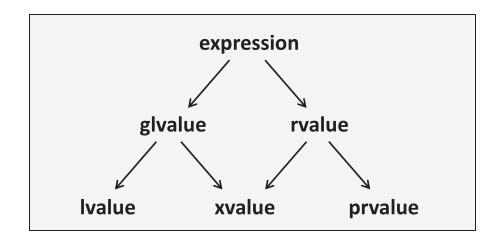
\includegraphics[scale=0.8]{../imgs/05.1.png}
    \caption{从C++11起的值类型体系}
    \label{f5.1}
\end{figure}

\emph{\textbf{lvalue(左值)}}的例子有:
\begin{itemize}
    \item 只含有单个变量、函数或成员(除了右值的普通值成员)的表达式
    \item 只含有字符串字面量的表达式
    \item 内建的一元\texttt{*}运算符(解引用运算符)的结果
    \item 一个返回lvalue(左值)引用(\emph{type\&})的函数的返回值
    \item 对函数的任何引用,即使使用\texttt{std::move()}标记
\end{itemize}
\emph{\textbf{prvalue(纯右值)}}的例子有:
\begin{itemize}
    \item 除字符串字面量和用户自定义字面量之外的字面量组成的表达式
    \item 内建的一元\texttt{\&}运算符(取地址运算符)的运算结果
    \item 内建的数学运算符的结果
    \item 一个返回值的函数的返回值
    \item 一个lambda表达式
\end{itemize}
\emph{\textbf{xvalue(到期值)}}的例子有:
\begin{itemize}
    \item 一个返回rvalue(右值)引用(\emph{type\&\&})的函数的返回值
    (尤其是\texttt{std::move()}的返回值)
    \item 把一个对象转换为rvalue(右值)引用的操作的结果
    \item rvalue(右值)的非静态值成员
\end{itemize}
简单来讲:
\begin{itemize}
    \item 所有用作表达式的变量名都是\emph{lvalue(左值)}。
    \item 所有用作表达式的字符串字面量是\emph{lvalue(左值)}。
    \item 所有其他的字面量(\texttt{4.2, true, nullptr})是\emph{prvalue(纯右值)}。
    \item 所有临时对象(尤其是以值返回的对象)是\emph{prvalue(纯右值)}。
    \item \texttt{std::move()}的结果是一个\emph{xvalue(到期值)}
\end{itemize}
例如:
\begin{lstlisting}
    class X {
    };
    X v;
    const X c;

    void f(const X&);   // 接受任何值类型
    void f(X&&);        // 只接受prvalue和xvalue,但是相比上边的版本是更好的匹配

    f(v);               // 给第一个f()传递了一个可修改lvalue
    f(c);               // 给第一个f()传递了不可修改的lvalue
    f(X());             // 给第二个f()传递了一个prvalue
    f(std::move(v));    // 给第二个f()传递了一个xvalue
\end{lstlisting}
值得强调的一点是严格来讲glvalue(广义左值)、prvalue(纯右值)、xvalue(到期值)是描述表达式的术语
而\emph{不是}描述值的术语(这意味着这些术语其实是误称)。例如,一个变量自身并不是左值,
只含有这个变量的表达式才是左值:
\begin{lstlisting}
    int x = 3;  // 这里,x是一个变量,不是一个左值
    int y = x;  // 这里,x是一个左值
\end{lstlisting}
在第一条语句中,\texttt{3}是一个纯右值,用它初始化了变量(不是左值)\texttt{x}。
在第二条语句中,\texttt{x}是一个左值(该表达式的求值结果指向一个包含有数值\texttt{3}的对象)。
左值\texttt{x}被转换为一个纯右值,然后用来初始化\texttt{y}。

\subsection{自从C++17起的值类型体系}
C++17再次明确了值类型体系,现在的值类型体系如\hyperref[f5.2]{图5.2}所示:

\begin{figure}[htb]
    \begin{center}
        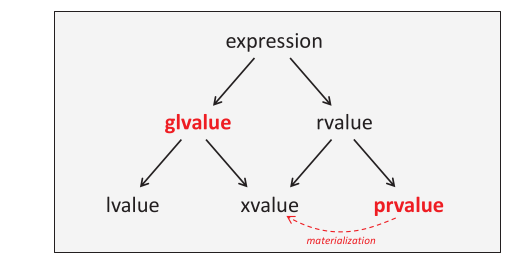
\includegraphics[scale=0.8]{../imgs/05.2.png}
        \caption{自从C++17起的值类型体系}
        \label{f5.2}
    \end{center}
\end{figure}

理解值类型体系的关键是现在广义上来说,我们只有两种类型的表达式:
\begin{itemize}
    \item \textbf{glvaue:} 描述对象或函数\emph{位置}的表达式
    \item \textbf{prvalue:} 用于\emph{初始化}的表达式
\end{itemize}
而\textbf{xvalue}可以认为是一种特殊的位置,它代表一个资源可以被回收利用的对象
(通常是因为该对象的生命周期即将结束)。

C++17引入了一个新的术语:(临时对象的)\emph{实质化(materialization)},
目前prvalue就是一种临时对象。
因此,\emph{临时对象实质化转换(temporary materialization conversion)}
是一种prvalue到xvalue的转换。

在任何情况下prvalue出现在需要glvalue(lvalue或者xvalue)的地方都是有效的,
此时会创建一个临时对象并用该prvalue来初始化(注意prvalue主要就是用来初始化的值)。
然后该prvalue会被临时创建的xvalue类型的临时对象替换。因此上面的例子严格来讲是这样的:
\begin{lstlisting}
    void f(const X& p); // 接受一个任何值类型体系的表达式
                        // 但实际上需要一个glvalue
    f(X());             // 传递了一个prvalue,该prvalue实质化为xvalue
\end{lstlisting}
因为这个例子中的\texttt{f()}的形参是一个引用,所以它需要glvaue类型的实参。
然而,表达式\texttt{X()}是一个prvalue。此时“临时变量实质化”规则会产生作用,
表达式\texttt{X()}会“转换为”一个xvalue类型的临时对象。

注意实质化的过程中并没有创建新的/不同的对象。左值引用\texttt{p}仍然\emph{绑定到}
xvalue和prvalue,尽管后者现在会转换为一个xvalue。

因为prvalue不再是对象而是可以被用来初始化对象的表达式,
所以当使用prvalue来初始化对象时不再需要prvalue是可移动的,
进而省略临时变量拷贝的特性可以完美实现。
我们现在只需要简单的传递初始值,然后它会被自动\emph{实质化}来初始化新对象。
\footnote{感谢Richard Smith和Graham Haynes指出这一点}


\section{未实质化的返回值传递}
所有以值返回临时对象(prvalue)的过程都是在传递未实质化的返回值:
\begin{itemize}
    \item 当我们返回一个非字符串字面量的字面量时:
    \begin{lstlisting}
    int f1() {  // 以值返回int
        return 42;
    }
    \end{lstlisting}
    \item 当我们用\texttt{auto}或类型名作为返回类型并返回一个临时对象时:
    \begin{lstlisting}
    auto f2() { // 以值返回退化的类型
        ...
        return MyType{...};
    }
    \end{lstlisting}
    \item 当使用\texttt{decltype(auto)}作为返回类型并返回临时对象时:
    \begin{lstlisting}
    decltype(auto) f3() {   // 返回语句中以值返回临时对象
        ...
        return MyType{...}
    }
    \end{lstlisting}
\end{itemize}

注意当初始化表达式(此处是返回语句)是一个创建临时对象(prvalue)的表达式时
\texttt{decltype(auto)}将会推导出值类型。因为我们在这些场景中都是以值返回一个prvalue,
所以我们完全不需要任何拷贝/移动。


\section{后记}
用临时变量初始化时强制省略拷贝由Richard Smith在\url{https://wg21.link/p0135r0}中首次提出。
最终被接受的是Richard Smith发表于\url{https://wg21.link/p0135r1}的提案。
    \section{lambda表达式扩展}\label{ch6}
lambda表达式是一个很大的成功,它最早在C++11中引入,在C++14中又引入了泛型lambda。
它允许我们将函数作为参数传递,这让我们能更轻易的指明一种行为。

C++17扩展了lambda表达式的应用场景:
\begin{itemize}[leftmargin=*]
    \item 在常量表达式中使用(也就是在编译期间使用)
    \item 在需要当前对象的拷贝时使用(例如,当在不同的线程中调用lambda时)
\end{itemize}

\subsection{\texttt{constexpr} lambda}
自从C++17起,lambda表达式会尽可能的隐式声明\texttt{constexpr}。
也就是说,任何只使用有效的编译期上下文
(例如,只有字面量,没有静态变量,没有虚函数,没有\texttt{try/catch},
没有\texttt{new/delete}的上下文)的lambda都可以被用于编译期。

例如,你可以使用一个lambda表达式计算参数的平方,并将计算结果用作\texttt{std::array<>}的大小,
即使这是一个编译期的参数:
\begin{lstlisting}
    auto squared = [](auto val) {   // 自从C++17起隐式constexpr
        return val*val;
    };
    std::array<int, squared(5)> a;  // 自从C++17起OK => std::array<int, 25>
\end{lstlisting}
使用\texttt{constexpr}中不允许的特性将会使lambda失去成为\texttt{constexpr}的能力,
不过你仍然可以在运行时上下文中使用lambda:
\begin{lstlisting}
    auto squared2 = [](auto val) {  // 自从C++17起隐式constexpr
        static int calls = 0;   // OK,但会使该lambda不能成为constexpr
        ...
        return val*val;
    };
    std::array<int, squared2(5)> a;     // ERROR:在编译期上下文中使用了静态变量
    std::cout << squared2(5) << '\n';   // OK
\end{lstlisting}
为了确定一个lambda是否能用于编译期,你可以将它声明为\texttt{constexpr}:
\begin{lstlisting}
    auto squared3 = [](auto val) constexpr {  // 自从C++17起OK
        return val*val;
    };
\end{lstlisting}
如果指明返回类型的话,看起来像下面这样:
\begin{lstlisting}
    auto squared3i = [](int val) constexpr -> int {  // 自从C++17起OK
        return val*val;
    };
\end{lstlisting}
关于\texttt{constexpr}函数的规则也适用于lambda:如果一个lambda在运行时上下文中使用,
那么相应的函数体也会在运行时才会执行。

然而,如果在声明了\texttt{constexpr}的lambda内使用了编译期上下文中不允许出现的特性
将会导致编译错误:\footnote{不允许出现在编译期上下文中的特性有:静态变量、虚函数、
\texttt{try/catch}、\texttt{new/delete}等。}
\begin{lstlisting}
    auto squared4 = [](auto val) constexpr {
        static int calls = 0;  // ERROR:在编译期上下文中使用了静态变量
        ...
        return val*val;
    };
\end{lstlisting}
一个隐式或显式的\texttt{constexpr} lambda的函数调用符也是\texttt{constexpr}。
也就是说,如下定义:
\begin{lstlisting}
    auto squared = [](auto val) {   // 自从C++17起隐式constexpr
        return val*val;
    };
\end{lstlisting}
将会被转换为如下\emph{闭包类型}(closure type):
\begin{lstlisting}
    class CompilerSpecificName {
      public:
        ...
        template<typename T>
        constexpr auto operator() (T val) const {
            return val*val;
        }
    };
\end{lstlisting}
注意,这里自动生成的闭包类型的函数调用运算符自动声明为\texttt{constexpr}。
自从C++17起,如果lambda被显式或隐式地定义为\texttt{constexpr},
那么生成的函数调用运算符将自动是\texttt{constexpr}。
注意如下定义:
\begin{lstlisting}
    auto squared1 = [](auto val) constexpr {  // 编译期lambda调用
        return val*val;
    };
\end{lstlisting}
和如下定义:
\begin{lstlisting}
    constexpr auto squared2 = [](auto val) {  // 编译期初始化squared2
        return val*val;
    };
\end{lstlisting}
是不同的。

第一个例子中如果(只有)lambda是\texttt{constexpr}那么它可以被用于编译期,
但是\texttt{squared1}可能直到运行期才会被初始化,
这意味着如果静态初始化顺序很重要那么可能导致问题。
如果用lambda初始化的闭包对象是\texttt{constexpr},那么该对象将在程序开始时就初始化,
但lambda可能还是只能在运行时使用。因此,可以考虑使用如下定义:
\begin{lstlisting}
    constexpr auto squared = [](auto val) constexpr {
        return val*val;
    };
\end{lstlisting}

\subsubsection{使用\texttt{constexpr} lambda}
这里有一个使用\texttt{constexpr} lambda的例子。
假设我们有一个字符串的哈希函数,这个函数迭代字符串的每一个字符反复更新哈希值:
\footnote{djb2算法的源码见\url{http://www.cse.yorku.ca/~oz/hash.html}。}
\begin{lstlisting}
    auto hashed = [](const char* str) {
        std::size_t hash = 5381;    // 初始化哈希值
        while (*str != '\0') {
            hash = hash * 33 ^ *str++;  // 根据下一个字符更新哈希值
        }
        return hash;
    };
\end{lstlisting}
使用这个lambda,我们可以在编译期初始化不同字符串的哈希值,并定义为枚举:
\begin{lstlisting}
    enum Hashed { beer = hashed("beer"),
                  wine = hashed("wine"),
                  water = hashed("water"),
                  ... };   // OK,编译期哈希
\end{lstlisting}
我们也可以在编译期计算\texttt{case}标签:
\begin{lstlisting}
    switch (hashed(argv[1])) {  // 运行时哈希
        case hashed("beer"):    // OK,编译期哈希
            ...
            break;
        case hashed("wine"):
            ...
            break;
        ...
    }
\end{lstlisting}
注意,这里我们将在编译期调用\texttt{case}标签里的\texttt{hashed},
而在运行期间调用\texttt{switch}表达式里的\texttt{hashed}。

如果我们使用编译期lambda初始化一个容器,那么编译器优化时很可能在编译期就计算出容器的初始值
(这里使用了\hyperref[ch9.2.6.3]{\texttt{std::array}的类模板参数推导}):
\begin{lstlisting}
    std::array arr{ hashed("beer"),
                    hashed("wine"),
                    hashed(("water")};
\end{lstlisting}
你甚至可以在\texttt{hashed}函数里联合使用另一个\texttt{constexpr} lambda。
设想我们把\texttt{hashed}里根据当前哈希值和下一个字符值更新哈希值的逻辑定义为一个参数:
\begin{lstlisting}
    auto hashed = [](const char* str, auto combine) {
        std::size_t hash = 5381;
        while (*str != '\0') {
            hash = combine(hash, *str++);   // 用下一个字符更新哈希值
        }
        return hash;
    };
\end{lstlisting}
这个lambda可以像下面这样使用:
\begin{lstlisting}
    constexpr std::size_t hv1{
        hashed("wine"), [](auto h, char c) {return h*33 + c;})};
    constexpr std::size_t hv2{
        hashed("wine"), [](auto h, char c) {return h*33 ^ c;})};
\end{lstlisting}
这里,我们在编译期通过改变更新逻辑初始化了两个不同的"wine"的哈希值。
两个\texttt{hashed}都是在编译期调用。

\subsection{向lambda传递\texttt{this}的拷贝}
当在非静态成员函数里使用lambda时,你不能隐式获取对该对象成员的使用权。
也就是说,如果你不捕获\texttt{this}的话你将不能在lambda里使用该对象的任何成员
(即使你用\texttt{this->}来访问也不行):
\begin{lstlisting}
    class C {
      private:
        std::string name;
      public:
        ...
        void foo() {
            auto l1 = [] {std::cout << name << '\n';}; // ERROR
            auto l2 = [] {std::cout << this->name << '\n';}; // ERROR
            ...
        }
    };
\end{lstlisting}
在C++11和C++14里,你可以通过值或引用捕获\texttt{this}:
\begin{lstlisting}
    class C {
      private:
        std::string name;
      public:
        ...
        void foo() {
            auto l1 = [this] {std::cout << name << '\n';}; // OK
            auto l2 = [=] {std::cout << name << '\n';}; // OK
            auto l3 = [&] {std::cout << name << '\n';}; // OK
            ...
        }
    };
\end{lstlisting}
然而,问题是即使是用拷贝的方式捕获\texttt{this}实质上获得的也是引用
(因为只会拷贝\texttt{this}指针)。当lambda的生命周期比该对象的生命周期更长的时候,
调用这样的函数就可能导致问题。比如一个极端的例子是在lambda中开启一个新的线程来完成某些任务,
调用新线程时正确的做法是传递整个对象的拷贝来避免并发和生存周期的问题,而不是传递该对象的引用。
另外有时候你可能只是简单的想向lambda传递当前对象的拷贝。

自从C++14起有了一个解决方案,但可读性和实际效果都比较差:
\begin{lstlisting}
    class C {
      private:
        std::string name;
      public:
        ...
        void foo() {
            auto l1 = [thisCopy=*this]
                { std::cout << thisCopy.name << '\n'; };
            ...
        }
    };
\end{lstlisting}
例如,当使用了\texttt{=}或者\texttt{\&}捕获了其他对象的时候你可能会在不经意间使用\texttt{this}:
\begin{lstlisting}
    auto l1 = [&, thisCopy=*this] {
        thisCopy.name = "new name";
        std::cout << name << '\n'; // OOPS:仍然使用了原来的name
    };
\end{lstlisting}
自从C++17起,你可以通过\texttt{*this}显式地捕获当前对象的拷贝:
\begin{lstlisting}
    class C {
      private:
        std::string name;
      public:
        ...
        void foo() {
            auto l1 = [*this] { std::cout << name << '\n'; };
            ...
        }
    };
\end{lstlisting}
这里,捕获\texttt{*this}意味着该lambda生成的闭包将存储当前对象的一份\emph{拷贝}。

你仍然可以在捕获\texttt{*this}的同时捕获其他对象,只要没有多个\texttt{this}的矛盾:
\begin{lstlisting}
    auto l2 = [&, *this] { ... };       // OK
    auto l3 = [this, *this] { ... };    // ERROR
\end{lstlisting}
这里有一个完整的例子:
\inputcodefile{lang/lambdathis.cpp}
lambda里捕获了\texttt{*this},因此传递进lambda的是一份拷贝。
因此,即使在\texttt{d}被销毁之后使用捕获的对象也没有问题。

如果我们使用\texttt{[this]}、\texttt{[=]}或者\texttt{[\&]}捕获\texttt{this},
那么新线程将会陷入未定义行为,因为当线程中打印\texttt{name}的时候将会使用一个已经销毁的
对象的成员。

\subsection{以常量引用捕获}
通过使用一个新的库工具,现在也可以\nameref{ch25.2.1}。

\subsection{后记}
\texttt{constexpr} lambda最早由Faisal Vali、Ville Voutilainen和Gabriel Dos Reis
在\url{https://wg21.link/n4487}中首次提出。
最终被接受的正式提案由Faisal Vali、Jens Maurer、Richard Smith
发表于\url{https://wg21.link/p0170r1}。

\setcounter{footnote}{0}
    \section{新属性和属性特性}\label{ch7}
自从C++11起,就可以指明\emph{属性}(attribute)(允许或者禁用某些警告的注解)。
C++17引入了新的属性,另外现在属性也可以在其他一些地方使用,也许能带来一些便利。

\subsection{\texttt{[[nodiscard]]}属性}
新属性\texttt{[[nodiscard]]}可以鼓励编译器在某个函数的返回值未被使用时给出警告
(这并不意味着编译器一定要给出警告)。
\texttt{[[nodiscard]]}通常应该用于防止某些因为返回值未被使用导致的不当行为。
这些不当行为可能是(译者注:请配合下边的例子理解这些不当行为):
\begin{itemize}[leftmargin=*]
    \item \textbf{内存泄露},例如返回值中含有动态分配的内存,但并未使用。
    \item \textbf{未知的或出乎意料的行为},例如因为没有使用返回值而导致了一些奇怪的行为。
    \item \textbf{不必要的开销},例如因为返回值没被使用而进行了一些无意义的行为。
\end{itemize}
这里有一些该属性发挥所用的例子:
\begin{itemize}[leftmargin=*]
    \item 申请资源但自身并不释放,而是将资源返回等待其他函数释放的函数应该被标记为
    \texttt{[[nodiscard]]}。一个典型的例子是申请内存的函数,
    例如\texttt{malloc()}函数或者分配器的\texttt{allocate()}成员函数。

    然而,注意有些函数\emph{可能}会返回一个无需再处理的值。例如,程序员可能会用0字节调用C函数
    \texttt{realloc()}来释放内存,这种情况下的返回值无需之后调用\texttt{free()}函数释放。
    因此,如果对\texttt{realloc()}标记\texttt{[[nodiscard]]}将会适得其反。
    \item 有时如果没有使用返回值将导致函数行为和预期不同,一个很好的例子是\texttt{std::async()}
    (C++11引入)。\texttt{std::async()}会在后台异步地执行一个任务并返回一个可以用来等待
    任务执行结束的句柄(也可以通过它获取返回值或者异常)。然而,如果返回值没有被使用的话该调用
    将变成同步的调用,因为在启动任务的语句结束之后未被使用的返回值的析构函数会立即执行,而析构
    函数会阻塞等待任务运行结束。因此,不使用返回值导致的结果与\texttt{std::async()}的目的
    完全矛盾。将\texttt{std::async()}标记为\texttt{[[nodiscard]]}可以让编译器给出警告。
    \item 另一个例子是成员函数\texttt{empty()},它的作用是检查一个对象(容器/字符串)是否
    没有元素。程序员经常误用该函数来“清空“容器:
    \begin{lstlisting}
    cont.empty();
    \end{lstlisting}
    这种对\texttt{empty()}的误用并没有使用返回值,所以\texttt{[[nodiscard]]}可以检查出这种误用:
    \begin{lstlisting}
    class MyContainer {
        ...
      public:
        [[nodiscard]] bool empty() const noexcept;
        ...
    };
    \end{lstlisting}
    这里的属性标记可以帮助检查这种逻辑错误。
\end{itemize}
如果因为某些原因你不想使用一个被标记为\texttt{[[nodiscard]]}的函数的返回值,
你可以把返回值转换为\texttt{void}:
\begin{lstlisting}
    (void)coll.empty(); // 禁止[[nodiscard]]警告
\end{lstlisting}
注意如果成员函数被覆盖或者隐藏时基类中标记的属性不会被继承:
\begin{lstlisting}
    struct B {
        [[nodiscard]] int* foo();
    };

    struct D : B {
        int* foo();
    };

    B b;
    b.foo();        // 警告
    (void)b.foo();  // 没有警告

    D d;
    d.foo();        // 没有警告
\end{lstlisting}
因此你需要给派生类里相应的成员函数再次标记\texttt{[[nodiscard]]}
(除非有某些原因导致你不想在派生类里确保返回值必须被使用)。

你可以把属性标记在函数前的所有修饰符之前,也可以标记在函数名之后:
\begin{lstlisting}
    class C {
        ...
        [[nodiscard]] friend bool operator== (const C&, const C&);
        friend bool operator!= [[nodiscard]] (const C&, const C&);
    };
\end{lstlisting}
把属性放在\texttt{friend}和\texttt{bool}之间或者\texttt{bool}和\texttt{operator==}
之间是错误的。

尽管这个特性从C++17起引入,但它还没有在标准库中使用。因为这个提案出现的太晚了,所以最应该
需要它的\texttt{std::async()}也还没有使用它。不过这里讨论的所有例子,将在下一次C++标准
中实现(见C++20中通过的\url{https://wg21.link/p0600r1}提案)。

为了保证代码的可移植性,你应该使用\texttt{[[nodiscard]]}而不是一些不可移植的方案
(例如gcc和clang的\texttt{[[gnu:warn\_unused\_result]]}或者Visual C++的
\texttt{\_Check\_return\_})。

当\hyperref[ch30.2.2]{定义\texttt{new()}运算符}时,
你应该用\texttt{[[nodiscard]]}对该函数进行标记,
例如\hyperref[ch30.4]{定义一个追踪所有\texttt{new}调用的头文件}。

\subsection{\texttt{[[maybe\_unused]]}属性}
新的属性\texttt{[[maybe\_unused]]}可以避免编译器在某个变量未被使用时发出警告。
新的属性可以应用于类的声明、使用\texttt{typedef}或者\texttt{using}定义的类型、
一个变量、一个非静态数据成员、一个函数、一个枚举类型、一个枚举值等场景。

例如其中一个作用是定义一个可能不会使用的参数:
\begin{lstlisting}
    void foo(int val, [[maybe_unused]] std::string msg)
    {
    #ifdef DEBUG
        log(msg);
    #endif
        ...
    }
\end{lstlisting}
另一个例子是定义一个可能不会使用的成员:
\begin{lstlisting}
    class MyStruct {
        char c;
        int i;
        [[maybe_unused]] char makeLargerSize[100];
        ...
    };
\end{lstlisting}
注意你不能在一条语句上应用\texttt{[[maybe\_unused]]}。
也就是说,你不能直接用\texttt{[[maybe\_unused]]}来抵消\texttt{[[nodiscard]]}的作用:
\footnote{感谢Roland Bock指出这一点}
\begin{lstlisting}
    [[nodiscard]] void* foo();
    int main()
    {
        foo();  // 警告:返回值没有使用
        [[maybe_unused]] foo(); // 错误:maybe_unused不允许出现在此
        [[maybe_unused]] auto x = foo(); // OK
    }
\end{lstlisting}

\subsection{\texttt{[[fallthrough]]}属性}
新的属性\texttt{[[fallthrough]]}可以避免编译器在\texttt{switch}语句中某一个标签
缺少\texttt{break}语句时发出警告。例如:
\begin{lstlisting}
    void commentPlace(int place)
    {
        switch (place) {
            case 1:
                std::cout << "very ";
                [[fallthrough]];
            case 2:
                std::cout << "well\n";
                break;
            default:
                std::cout << "OK\n";
                break;
        }
    }
\end{lstlisting}
这个例子中参数为1时将输出:
\begin{lstlisting}
    very well
\end{lstlisting}
\texttt{case 1}和\texttt{case 2}中的语句都会被执行。
注意这个属性必须被用作单独的语句,还要有分号结尾。
另外在\texttt{switch}语句的最后一个分支不能使用它。

\subsection{通用的属性扩展}
自从C++17起下列有关属性的通用特性变得可用:
\begin{enumerate}[leftmargin=*]
    \item 属性现在可以用来标记命名空间。例如,你可以像下面这样弃用一个命名空间:
    \begin{lstlisting}
    namespace [[deprecated]] DraftAPI {
        ...
    }
    \end{lstlisting}
    这也可以应用于内联的和匿名的命名空间。
    \item 属性现在可以标记枚举子(枚举类型的值)。
    例如你可以像下面这样引入一个新的枚举值作为某个已有枚举值(并且现在已经被废弃)的替代:
    \begin{lstlisting}
    enum class City { Berlin = 0,
        NewYork = 1,
        Mumbai = 2,
        Bombay [[deprecated]] = Mumbai,
        ... };
    \end{lstlisting}
    这里\texttt{Mumbai}和\texttt{Bombay}代表同一个城市的数字码,但使用\texttt{Bombay}
    已经被标记为废弃的。注意对于枚举值,属性被放置在标识符\emph{之后}。
    \item 用户自定义的属性一般应该定义在自定义的命名空间中。现在可以使用\texttt{using}前缀
    来避免为每一个属性重复输入命名空间。也就是说,如下代码:
    \begin{lstlisting}
    [[MyLib::WebService, MyLib::RestService, MyLib::doc("html")]] void foo();
    \end{lstlisting}
    可以被替换为
    \begin{lstlisting}
    [[using MyLib: WebService, RestService, doc("html")]] void foo();
    \end{lstlisting}
    注意在使用了\texttt{using}前缀时重复命名空间将导致错误:
    \begin{lstlisting}
    [[using MyLib: MyLib::doc("html")]] void foo(); // ERROR
    \end{lstlisting}
\end{enumerate}

\subsection{后记}
三个新属性由Andrew Tomazos在\url{https://wg21.link/p0068r0}中首次提出。

\texttt{[[nodiscard]]}最终被接受的提案由Andrew Tomazos发表于
\url{https://wg21.link/p0189r1}。

\texttt{[[maybe\_unused]]}最终被接受的提案由Andrew Tomazos发表于
\url{https://wg21.link/p0212r1}。

\texttt{[[fallthrough]]}最终被接受的提案由Andrew Tomazos发表于
\url{https://wg21.link/p0188r1}。

允许为命名空间和枚举值标记属性的特性由Richard Smith在\url{https://wg21.link/n4196}
中首次提出。该特性最终被接受的提案由Richard Smith发表于\url{https://wg21.link/n4266}。

属性的\texttt{using}前缀由J. Daniel Garcia、Luis M. Sanchez、
Massimo Torquati、Marco Danelutto、Peter Sommerlad在\url{https://wg21.link/p0028r0}
中首次提出。最终被接受的提案由J. Daniel Garcia和Daveed Vandevoorde发表于
\url{https://wg21.link/P0028R4}。
    \chapter{其他语言特性}\label{ch8}
在C++17中还有一些微小的核心语言特性的变更,将在这一章中介绍。

\section{嵌套命名空间}\label{ch8.1}
自从2003年第一次提出,到现在C++标准委员会终于同意了以如下方式定义嵌套的命名空间:
\begin{lstlisting}
    namespace A::B::C {
        ...
    }
\end{lstlisting}
等价于:
\begin{lstlisting}
    namespace A {
        namespace B {
            namespace C {
                ...
            }
        }
    }
\end{lstlisting}
注意目前还没有对嵌套内联命名空间的支持。
这是因为\texttt{inline}是作用于最内层还是整个命名空间还有歧义(两种情况都很有用)。

\section{有定义的表达式求值顺序}\label{ch8.2}
许多C++书籍里的代码如果按照直觉来看似乎是正确的,但严格上讲它们有可能导致未定义的行为。
一个简单的例子是在一个字符串中替换多个子串:
\begin{lstlisting}
    std::string s = "I heard it even works if you don't believe";
    s.replace(0, 8, "").replace(s.find("even", 4, "sometimes")
                       .replace(s.find("you don't"), 9, "I");
\end{lstlisting}
通常的假设是前8个字符被空串替换,\texttt{"even"}被\texttt{"sometimes"}替换,
\texttt{"you don't"}被\texttt{"I"}替换。因此结果是:
\begin{blacklisting}
    it sometimes works if I believe
\end{blacklisting}
然而在C++17之前最后的结果实际上并没有任何保证。因为查找子串位置的\texttt{find()}
函数可能在需要它们的返回值之前的任意时刻调用,而不是像直觉中的那样从左向右按顺序执行表达式。
事实上,所有的\texttt{find()}调用可能在执行第一次替换之前就全部执行,因此结果变为:

\begin{blacklisting}
    it even worsometimesf youIlieve
\end{blacklisting}
其他的结果也是有可能的:
\begin{blacklisting}
    it sometimes workIdon’t believe
    it even worsometiIdon’t believe
\end{blacklisting}
作为另一个例子,考虑使用输出运算符打印几个相互依赖的值:
\begin{lstlisting}
    std::cout << f() << g() << h();
\end{lstlisting}
通常的假设是依次调用\texttt{f()}、\texttt{g()}、\texttt{h()}函数。
然而这个假设实际上是错误的。\texttt{f()}、\texttt{g()}、\texttt{h()}有可能以任意顺序调用,
当这三个函数的调用顺序会影响返回值的时候可能就会出现奇怪的结果。

作为一个具体的例子,直到C++17之前,下面代码的行为都是未定义的:
\begin{lstlisting}
    i = 0;
    std::cout << ++i << ' ' << --i << '\n';
\end{lstlisting}
在C++17之前,它\emph{\textbf{可能}}会输出\texttt{1 0},但也可能输出\texttt{0 -1}
或者\texttt{0 0},这和变量\texttt{i}是\texttt{int}还是用户自定义类型无关(不过对于基本类型,
编译器一般会在这种情况下给出警告)。

为了解决这种未定义的问题,C++17标准重新定义了\emph{一些}运算符的的求值顺序,
因此这些运算符现在有了固定的求值顺序:
\begin{itemize}
    \item 对于运算
    \begin{lstlisting}
    e1 `\textbf{[}` e2 `\textbf{]}`
    e1 `\textbf{.}` e2
    e1 `\textbf{.*}` e2
    e1 `\textbf{->*}` e2
    e1 `\textbf{<<}` e2
    e1 `\textbf{>>}` e2
    \end{lstlisting}
    \emph{e1}现在保证一定会在\emph{e2}之前求值,因此求值顺序是从左向右。
    然而,注意同一个函数调用中的不同参数的计算顺序仍然是未定义的。也就是说:
    \begin{lstlisting}
    e1.f(a1, a2, a3);
    \end{lstlisting}
    中的\texttt{e1}保证会在\texttt{a1}、\texttt{a2}、\texttt{a3}之前求值。
    但\texttt{a1}、\texttt{a2}、\texttt{a3}的求值顺序仍是未定义的。
    \item 所有的赋值运算
    \begin{lstlisting}
    e2 `\textbf{=}` e1
    e2 `\textbf{+=}` e1
    e2 `\textbf{*=}` e1
    ...
    \end{lstlisting}
    中右侧的\emph{e1}现在保证一定会在左侧的\emph{e2}之前求值。
    \item 最后,类似于如下的\texttt{new}表达式
    \begin{lstlisting}
    `\textbf{new}` Type(e)
    \end{lstlisting}
    中保证内存分配的操作在对\emph{e}求值之前发生。
    新的对象的初始化操作保证在第一次使用该对象之前完成。
\end{itemize}
所有这些保证适用于所有基本类型和自定义类型。

因此,自从C++17起
\begin{lstlisting}
    std::string s = "I heard it even works if you don't believe";
    s.replace(0, 8, "").replace(s.find("even"), 4, "always")
                       .replace(s.find("don't believe"), 13, "use C++17");
\end{lstlisting}
保证将会把\texttt{s}的值修改为:
\begin{blacklisting}
    it always works if you use C++17
\end{blacklisting}
因为现在每个\texttt{find()}之前的替换操作都保证
会在对该\texttt{find()}表达式求值之前完成。

另一个例子,如下语句:
\begin{lstlisting}
    i = 0;
    std::cout << ++i << ' ' << --i << '\n';
\end{lstlisting}
对于任意类型的\texttt{i}都保证输出是\texttt{1 0}。

然而,其他大多数运算符的运算顺序仍然是未知的。例如:
\begin{lstlisting}
    i = i++ + i;    // 仍然是未定义的行为
\end{lstlisting}
这里,最右侧的\texttt{i}可能在\texttt{i}自增之前求值也可能在自增之后求值。

新的表达式求值顺序的另一个应用是定义一个在参数之前\hyperref[ch11.2.1]{插入空格的函数}。

\subsubsection{向后的不兼容性}
新的有定义的求值顺序可能会影响现有程序的输出。例如,考虑如下程序:
\inputcodefile{lang/evalexcept.cpp}
因为这个程序中的\texttt{vector<>}只有4个元素,因此在\texttt{print10elems()}的循环中
使用无效的索引调用\texttt{at()}时将会抛出异常:
\begin{lstlisting}
    std::cout << "value: " << v.at(i) << "\n";
\end{lstlisting}
在C++17之前,输出可能是:
\begin{blacklisting}
    value: 7
    value: 14
    value: 21
    value: 28
    EXCEPTION: ...
\end{blacklisting}
因为\texttt{at()}允许在输出\texttt{"value: "}之前调用,
所以当索引错误时可以跳过开头的\texttt{"value: "}输出。
\footnote{较旧版本的GCC或者Visual C++的行为就是这样的。}

自从C++17以后,输出保证是:
\begin{blacklisting}
    value: 7
    value: 14
    value: 21
    value: 28
    value: EXCEPTION: ...
\end{blacklisting}
因为现在\texttt{"value: "}的输出保证在\texttt{at()}调用之前。

\section{更宽松的用整型初始化枚举值的规则}\label{ch8.3}
对于一个有固定底层类型的枚举类型变量,自从C++17开始可以用一个整型值直接进行列表初始化。
这可以用于带有明确类型的无作用域枚举和所有有作用域的枚举,因为它们都有默认的底层类型:
\begin{lstlisting}
    // 指明底层类型的无作用域枚举类型
    enum MyInt : char { };
    MyInt i1{42};       // 自从C++17起OK(C++17以前ERROR)
    MyInt i2 = 42;      // 仍然ERROR
    MyInt i3(42);       // 仍然ERROR
    MyInt i4 = {42};    // 仍然ERROR

    // 带有默认底层类型的有作用域枚举
    enum class Weekday { mon, tue, wed, thu, fri, sat, sun };
    Weekday s1{0};      // 自从C++17起OK(C++17以前ERROR)
    Weekday s2 = 0;     // 仍然ERROR
    Weekday s3(0);      // 仍然ERROR
    Weekday s4 = {0};   // 仍然ERROR
\end{lstlisting}
如果\texttt{Weekday}有明确的底层类型的话结果完全相同:
\begin{lstlisting}
    // 带有明确底层类型的有作用域枚举
    enum class Weekday : char { mon, tue, wed, thu, fri, sat, sun };
    Weekday s1{0};      // 自从C++17起OK(C++17以前ERROR)
    Weekday s2 = 0;     // 仍然ERROR
    Weekday s3(0);      // 仍然ERROR
    Weekday s4 = {0};   // 仍然ERROR
\end{lstlisting}
对于\emph{没有}明确底层类型的无作用域枚举类型(没有\texttt{class}的\texttt{enum}),
你仍然不能使用列表初始化:
\begin{lstlisting}
    enum Flag { bit1=1, bit2=2, bit3=4 };
    Flag f1{0};     // 仍然ERROR
\end{lstlisting}
注意列表初始化不允许窄化,所以你不能传递一个浮点数:
\begin{lstlisting}
    enum MyInt : char { };
    MyInt i5{42.2}; // 仍然ERROR
\end{lstlisting}
一个定义新的整数类型的技巧是简单的定义一个以某个已有整数类型作为底层类型的枚举类型,
就像上面例子中的\texttt{MyInt}一样。
这个特性的动机之一就是为了支持这个技巧,如果没有这个特性,在不进行转换的情况下将无法初始化新的对象。

事实上自从C++17起标准库提供的\nameref{ch18}就直接使用了这个特性。

\section{修正\texttt{auto}类型的列表初始化}\label{ch8.4}
自从在C++11中引入了花括号\emph{统一}初始化之后,
每当使用\texttt{auto}代替明确类型进行列表初始化时就会出现一些和直觉不一致的结果:
\begin{lstlisting}
    int x{42};       // 初始化一个int
    int y{1, 2, 3};  // ERROR
    auto a{42};      // 初始化一个std::initializer_list<int>
    auto b{1, 2, 3}; // OK:初始化一个std::initializer_list<int>
\end{lstlisting}
这些\emph{直接}使用列表初始化(没有使用=)时的不一致行为现在已经被修复了。
因此如下代码的行为变成了:
\begin{lstlisting}
    int x{42};       // 初始化一个int
    int y{1, 2, 3};  // ERROR
    auto a{42};      // 现在初始化一个int
    auto b{1, 2, 3}; // 现在ERROR
\end{lstlisting}
注意这是一个\textbf{破坏性的更改(breaking change)},因为它可能导致很多代码的行为在
无声无息中发生改变。因此,支持了这个变更的编译器现在即使在C++11模式下也会启用这个变更。
对于主流编译器,接受这个变更的版本分别是Visual Studio 2015,g++5,clang3.8。

注意当使用\texttt{auto}进行\emph{拷贝列表初始化}(使用了=)时仍然是初始化一个
\texttt{std::initializer\_list<>}:
\begin{lstlisting}
    auto c = {42};      // 仍然初始化一个std::initializer_list<int>
    auto d = {1, 2, 3}; // 仍然OK:初始化一个std::initializer_list<int>
\end{lstlisting}
因此,现在直接初始化(没有=)和拷贝初始化(有=)之间又有了显著的不同:
\begin{lstlisting}
    auto a{42};     // 现在初始化一个int
    auto c = {42};  // 仍然初始化一个std::initializer_list<int>
\end{lstlisting}
这也是更推荐使用直接列表初始化(没有=的花括号初始化)的原因之一。

\section{十六进制浮点数字面量}\label{ch8.5}
C++17允许指定十六进制浮点数字面量(有些编译器甚至在C++17之前就已经支持)。
当需要一个精确的浮点数表示时这个特性非常有用(如果直接用十进制的浮点数字面量不保证
存储的实际精确值是多少)。

例如:
\inputcodefile{lang/hexfloat.cpp}
程序通过使用已有的和新增的十六进制浮点记号定义了不同的浮点数值。
新的记号是一个以2为基数的科学记数法记号:
\begin{itemize}
    \item 有效数字/尾数用十六进制书写
    \item 指数部分用十进制书写,表示乘以2的n次幂
\end{itemize}
例如\texttt{0xAp2}的值为40($10\times2^2$)。这个值也可以被写作\texttt{0x1.4p+5},
也就是$1.25\times32$(0.4是十六进制的分数,等于十进制的0.25,$2^5=32$)。

程序的输出如下:
\begin{blacklisting}
    dec:     16  hex: 0x1p+4
    dec:     10  hex: 0x1.4p+3
    dec:     40  hex: 0x1.4p+5
    dec:      5  hex: 0x1.4p+2
    dec:      5  hex: 0x1.4p+2
    dec: 100000  hex: 0x1.86ap+16
    dec: 100000  hex: 0x1.86ap+16
    dec: 49.625  hex: 0x1.8dp+5
\end{blacklisting}
就像上例展示的一样,十六进制浮点数的记号很早就存在了,
因为输出流使用的\texttt{std::hexfloat}操作符自从C++11起就已经存在了。

\section{UTF-8字符字面量}\label{ch8.6}
自从C++11起,C++就已经支持以\texttt{u8}为前缀的UTF-8字符串字面量。
然而,这个前缀不能用于字符字面量。C++17修复了这个问题,所以现在可以这么写:
\begin{lstlisting}
    auto c = u8'6'; // UTF-8编码的字符6
\end{lstlisting}
在C++17中,\texttt{u8'6'}的类型是\texttt{char},在C++20中可能会变为\texttt{char8\_t},
因此这里使用\texttt{auto}会更好一些。

通过使用该前缀现在可以保证字符值是UTF-8编码。你可以使用所有的7位的US-ASCII字符,
这些字符的UTF-8表示和US-ASCII表示完全相同。
也就是说,\texttt{u8'6'}也是有效的以7位US-ASCII表示的字符'6'
(也是有效的ISO Latin-1、ISO-8859-15、基本Windows字符集中的字符)。
\footnote{ISO Latin-1的正式命名为ISO-8859-1,而为了包含欧元符号€引入的字符集
ISO-8859-15也被命名为ISO Latin-9。}
通常情况下你的源码字符被解释为US-ASCII或者UTF-8的结果是一样的,所以这个前缀并不是必须的。
\texttt{c}的值永远是\texttt{54}(十六进制\texttt{36})。

这里给出一些背景知识来说明这个前缀的必要性:对于源码中的字符和字符串字面量,
C++标准化了你可以使用的字符而不是这些字符的值。这些值取决于\emph{源码字符集}。
当编译器为源码生成可执行程序时它使用\emph{运行字符集}。源码字符集几乎总是7位的
US-ASCII编码,而运行字符集通常是相同的。这意味着在任何C++程序中,所有相同的字符和字符串字面量
(不管有没有\texttt{u8}前缀)总是有相同的值。

然而,在一些特别罕见的场景中并不是这样的。例如,在使用EBCDIC字符集的旧的IBM机器上,字符'6'
的值将是246(十六进制为F6)。在一个使用EBCDIC字符集的程序中上面的字符\texttt{c}的值将是
246而不是54,如果在UTF-8编码的平台上运行这个程序可能会打印出字符ö,这个字符在ISO/IEC 8859-x
编码中的值为246.在这种情况下,这个前缀就是必须的。

注意\texttt{u8}只能用于单个字符,并且该字符的UTF-8编码必须只占一个字节。一个如下的初始化:
\begin{lstlisting}
    char c = u8'ö';
\end{lstlisting}
是不允许的,因为德语的曲音字符ö的UTF-8编码是两个字节的序列,分别是195和182(十六进制为C3 B6)。

因此,字符和字符串字面量现在接受如下前缀:
\begin{itemize}
    \item u8用于单字节US-ASCII和UTF-8编码
    \item u用于两字节的UTF-16编码
    \item U用于四字节的UTF-32编码
    \item L用于没有明确编码的宽字符,可能是两个或者四个字节
\end{itemize}

\section{异常声明作为类型的一部分}\label{ch8.7}
自从C++17之后,异常处理声明变成了函数类型的一部分。也就是说,如下的两个函数的类型是不同的:
\begin{lstlisting}
    void fMightThrow();
    void fNoexcept() noexcept;  // 不同类型
\end{lstlisting}
在C++17之前这两个函数的类型是相同的。这样的一个问题就是如果把一个可能抛出异常的函数赋给
一个保证不抛出异常的函数指针,那么调用时有可能会抛出异常:
\footnote{这样看起来好像是一个错误,但至少之前g++的确允许这种行为。}
\begin{lstlisting}
    void (*fp)() noexcept;  // 指向不抛异常的函数的指针
    fp = fNoexcept;         // OK
    fp = fMightThrow;       // 自从C++17起ERROR
\end{lstlisting}
把一个不会抛出异常的函数赋给一个可能抛出异常的函数指针仍然是有效的:
\begin{lstlisting}
    void (*fp2)();      // 指向可能抛出异常的函数的指针
    fp2 = fNoexcept;    // OK
    fp2 = fMightThrow;  // OK
\end{lstlisting}
因此,如果程序中只使用了没有\texttt{noexcept}声明的函数指针,那么将不会受该特性影响。
但请注意现在不能再违反函数指针中的\texttt{noexcept}声明(这可能会善意的破坏现有的程序)。

重载一个签名完全相同只有异常声明不同的函数是不允许的(就像不允许重载只有返回值不同的函数一样):
\begin{lstlisting}
    void f3();
    void f3() noexcept;     // ERROR
\end{lstlisting}
注意其他的规则不受影响。例如,你仍然不能忽略基类中的\texttt{noexcept}声明:
\begin{lstlisting}
    class Base {
    public:
        virtual void foo() noexcept;
        ...
    };

    class Derived : public Base {
    public:
        void foo() override;    // ERROR:不能重载
        ...
    };
\end{lstlisting}
这里,派生类中的成员函数\texttt{foo()}和基类中的\texttt{foo()}类型不同所以不能重载。
这段代码不能通过编译,即使没有\texttt{override}修饰符代码也不能编译,因为我们不能用
更宽松的异常声明重载。

\subsubsection{使用传统的异常声明}
当使用传统的\texttt{noexcept}声明时,函数的是否抛出异常取决于条件为true还是false:
\begin{lstlisting}
    void f1();
    void f2() noexcept;
    void f3() noexcept(sizeof(int)<4);  // 和f1()或f2()的类型相同
    void f4() noexcept(sizeof(int)>=4); // 和f3()的类型不同
\end{lstlisting}
这里\texttt{f3()}的类型取决于条件的值:
\begin{itemize}
    \item 如果\texttt{sizeof(int)}返回4或者更大,签名等价于
    \begin{lstlisting}
    void f3() noexcept(false); // 和f1()类型相同
    \end{lstlisting}
    \item 如果\texttt{sizeof(int)}返回的值小于4,签名等价于
    \begin{lstlisting}
    void f3() noexcept(true);  // 和f2()类型相同
    \end{lstlisting}
\end{itemize}
因为\texttt{f4()}的异常条件和\texttt{f3()}的恰好相反,所以\texttt{f3()}和\texttt{f4()}
的类型总是不同(也就是说,它们一定是一个可能抛异常,另一个不可能抛异常)。

旧式的不抛异常的声明仍然有效但自从C++11起就被废弃:
\begin{lstlisting}
    void f5() throw();  // 和void f5() noexcept等价但已经被废弃
\end{lstlisting}
带参数的动态异常声明不再被支持(自从C++11起被废弃):
\begin{lstlisting}
    void f6() throw(std::bad_alloc); // ERROR:自从C++17起无效
\end{lstlisting}

\subsubsection{对泛型库的影响}
将\texttt{noexcept}做为类型的一部分意味着会对泛型库产生一些影响。例如,下面的代码
直到C++14是有效的,但从C++17起不能再通过编译:
\inputcodefile{lang/noexceptcalls.cpp}
问题在于自从C++17起\texttt{f1()}和\texttt{f2()}的类型不再相同,
因此在实例化模板函数\texttt{call()时}编译器无法推导出类型\texttt{T},

自从C++17起,你需要指定两个不同的模板参数来通过编译:
\begin{lstlisting}
    template<typename T1, typename T2>
    void call(T1 op1, T2 op2)
    {
        op1();
        op2();
    }
\end{lstlisting}
现在如果你想重载所有可能的函数类型,那么你需要重载的数量将是原来的两倍。
例如,对于标准库类型特征\texttt{std::is\_function<>}的定义,
主模板的定义如下,该模板用于匹配\texttt{T}不是函数的情况:
\begin{lstlisting}
    // 主模板(匹配泛型类型T不是函数的情况):
    template<typename T> struct is_function : std::false_type { };
\end{lstlisting}
该模板从\hyperref[ch33.2]{\texttt{std::false\_type}}派生,
因此\texttt{is\_function<T>::value}对任何类型\texttt{T}都会返回\texttt{false}。

对于任何\emph{是}函数的类型,存在从\hyperref[ch33.2]{\texttt{std::true\_type}}
派生的部分特化版,因此成员\texttt{value}总是返回\texttt{true}:
\begin{lstlisting}
    // 对所有函数类型的部分特化版
    template<typename Ret, typename... Params>
    struct is_function<Ret (Params...)> : std::true_type { };

    template<typename Ret, typename... Params>
    struct is_function<Ret (Params...) const> : std::true_type { };

    template<typename Ret, typename... Params>
    struct is_function<Ret (Params...) &> : std::true_type { };

    template<typename Ret, typename... Params>
    struct is_function<Ret (Params...) const &> : std::true_type { };
    ...
\end{lstlisting}
在C++17之前该特征总共有24个部分特化版本:因为函数类型可以用\texttt{const}
和\texttt{volatile}修饰符修饰,另外还可能有左值引用(\&)或右值引用(\&\&)修饰符,
还需要重载可变参数列表的版本。

现在在C++17中部分特化版本的数量变为了两倍,因为还需要为所有版本添加一个带\texttt{noexcept}
修饰符的版本:
\begin{lstlisting}
    ...
    // 对所有带有noexcept声明的函数类型的部分特化版本
    template<typename Ret, typename... Params>
    struct is_function<Ret (Params...) noexcept> : std::true_type { };

    template<typename Ret, typename... Params>
    struct is_function<Ret (Params...) const noexcept> : std::true_type { };

    template<typename Ret, typename... Params>
    struct is_function<Ret (Params...) & noexcept> : std::true_type { };

    template<typename Ret, typename... Params>
    struct is_function<Ret (Params...) const & noexcept> : std::true_type { };
    ...
\end{lstlisting}
那些没有实现\texttt{noexcept}重载的库可能在需要使用带有
\texttt{noexcept}的函数的场景中不能通过编译了。

\section{单参数\texttt{static\_assert}}\label{ch8.8}
自从C++17起,以前\texttt{static\_assert()}要求的用作错误信息的参数变为可选的了。
也就是说现在断言失败时输出的诊断信息完全依赖平台的实现。例如:
\begin{lstlisting}
    #include <type_traits>

    template<typename t>
    class C {
        // 自从C++11起OK
        static_assert(std::is_default_constructible<T>::value,
                      "class C: elements must be default-constructible");

        // 自从C++17起OK
        static_assert(std::is_default_constructible_v<T>);
        ...
    };
\end{lstlisting}
不带错误信息参数的新版本静态断言的示例也使用了\nameref{ch21.1}。

\section{预处理条件\texttt{\_\_has\_include}}\label{ch8.9}
C++17扩展了预处理,增加了一个检查某个头文件是否可以被包含的宏。例如:
\begin{lstlisting}
    #if __has_include(<filesystem>)
    #  include <filesystem>
    #  define HAS_FILESYSTEM 1
    #elif __has_include(<experimental/filesystem>)
    #  include <experimental/filesystem>
    #  define HAS_FILESYSTEM 1
    #  define FILESYSTEM_IS_EXPERIMENTAL 1
    #elif __has_include("filesystem.hpp")
    #  include "filesystem.hpp"
    #  define HAS_FILESYSTEM 1
    #  define FILESYSTEM_IS_EXPERIMENTAL 1
    #else
    #  define HAS_FILESYSTEM 0
    #endif
\end{lstlisting}
当相应的\texttt{\#include}指令有效时\texttt{\_\_has\_include(...)}会被求值为1。
其他的因素都不会影响结果(例如,相应的头文件是否已被包含过并不影响结果)。

另外,虽然求值为真可以说明相应的头文件确实存在但不能保证它的内容符合预期。
它的内容可能是空的或者无效的。

\texttt{\_\_has\_include}是一个纯粹的预处理指令。
所以不能将它用作源码里的条件表达式:
\begin{lstlisting}
    if (__has_include(<filesystem>)) {  // ERROR
    }
\end{lstlisting}

\section{后记}
\hyperref[ch8.1]{嵌套命名空间定义}由Jon Jagger于2003年在
\url{https://wg21.link/n1524}中首次提出。
Robert Kawulak于\\
2014年在\url{https://wg21.link/n4026}中提出了新的提案。
最终被接受的是Robert Kawulak和Andrew Tomazos发表于\url{https://wg21.link/n4230}的提案。

\nameref{ch8.2}由Gabriel Dos Reis、Herb Sutter、Jonathan Caves在
\url{https://wg21.link/n4228}中首次提出。最终被接受的是Gabriel Dos Reis、
Herb Sutter和Jonathan Caves发表于\url{https://wg21.link/p0145r3}的提案。

\nameref{ch8.3}由Gabriel Dos Reis在\url{https://wg21.link/p0138r0}中首次提出。
最终被接受的是Gabriel Dos Reis发表于\url{https://wg21.link/p0138r2}的提案。

\nameref{ch8.4}由Ville Voutilainen在\url{https://wg21.link/n3681}以及
\url{https://wg21.link/3912}中首次提出。\texttt{auto}列表初始化最终的修正由
James Dennett在\url{https://wg21.link/n3681}提出。

\nameref{ch8.5}由Thomas Köppe在\url{https://wg21.link/p0245r0}中首次提出。
最终被接受的是Thomas Köppe发表于\url{https://wg21.link/p0245r1}的提案。

\nameref{ch8.6}是由Richard Smith在\url{https://wg21.link/n4197}中首次提出。
最终被接受的是Richard Smith发表于\url{https://wg21.link/n4267}的提案。

\nameref{ch8.7}由Jens Maurer在\url{https://wg21.link/n4320}中首次提出。
最终被接受的是Jens Maurer发表于\url{https://wg21.link/p0012r1}的提案。

\nameref{ch8.8}被接受的是Walter E. Brown发表于\url{https://wg21.link/n3928}的提案。

\hyperref[ch8.9]{预处理语句\texttt{\_\_has\_include()}}由Clark Nelson和Richard Smith在
\url{https://wg21.link/p0061r0}的某一部分中首次提出。
最终被接受的是Clark Nelson和Richard Smith发表于\url{https://wg21.link/p0061r1}的提案。



    \part{模板特性}\label{part2}
    这一部分介绍了C++17为泛型编程(即template)提供的新的语言特性。

    我们首先从类模板参数推导开始,这一特性只影响模板的使用。之后的章节会介绍为编写泛型代码(函数模板,
    类模板,泛型库等)的程序员提供的新特性。

    \chapter{类模板参数推导}\label{ch9}
在C++17之前,你必须明确指出类模板的所有参数。
例如,你不可以省略下面的\texttt{double}:
\begin{lstlisting}
    std::complex<double> c{5.1, 3.3};
\end{lstlisting}
也不可以省略下面的\texttt{std::mutex}:
\begin{lstlisting}
    std::mutex mx;
    std::lock_guard<std::mutex> lg(mx);
\end{lstlisting}
自从C++17起必须指明类模板参数的限制被放宽了。
通过使用\emph{类模板参数推导}(class template argument deduction)(CTAD),
只要编译器能根据初始值\emph{推导出}所有模板参数,那么就可以不指明参数。

例如:
\begin{itemize}
    \item 你现在可以这么声明:
    \begin{lstlisting}
    std::complex c{5.1, 3.3};   // OK:推导出std::complex<double>
    \end{lstlisting}
    \item 你现在可以这么写:
    \begin{lstlisting}
    std::mutex mx;
    std::lock_guard lg{mx}; // OK:推导出std::lock_guard<std::mutex>
    \end{lstlisting}
    \item 你现在甚至可以让容器来推导元素类型:
    \begin{lstlisting}
    std::vector v1{1, 2, 3}; // OK:推导出std::vector<int>
    std::vector v2{"hello", "world"}; // OK:推导出std::vector<const char*>
    \end{lstlisting}
\end{itemize}

\section{使用类模板参数推导}
只要能根据初始值推导出所有模板参数就可以使用类模板参数推导。
推导过程支持所有方式的初始化(只要保证初始化是有效的):
\begin{lstlisting}
    std::complex c1{1.1, 2.2};  // 推导出std::complex<double>
    std::complex c2(2.2, 3.3);  // 推导出std::complex<double>
    std::complex c3 = 3.3;      // 推导出std::complex<double>
    std::complex c4 = {4.4};    // 推导出std::complex<double>
\end{lstlisting}
因为\texttt{std::complex}只需要一个参数就可以初始化并推导出模板参数\texttt{T}:
\begin{lstlisting}
    namespace std {
        template<typename T>
        class complex {
            constexpr complex(const T&re = T(), const T& im = T());
            ...
        }
    };
\end{lstlisting}
所以\texttt{c3}和\texttt{c4}可以正确初始化。
对于如下声明:
\begin{lstlisting}
    std::complex c1{1.1, 2.2};
\end{lstlisting}
编译器会查找到构造函数:
\begin{lstlisting}
    constexpr complex(const T& re = T(), const T& im = T());
\end{lstlisting}
并调用。因为两个参数都是\texttt{double}类型,因此编译器会推导出\texttt{T}的就是
\texttt{double}并生成如下代码:
\begin{lstlisting}
    complex<double>::complex(const double& re = double(), const double& im = double());
\end{lstlisting}
注意推导的过程中模板参数必须没有歧义。也就是说,如下初始化代码不能通过编译:
\begin{lstlisting}
    std::complex c5{5, 3.3};    // ERROR:尝试将T推导为int和double
\end{lstlisting}
推导模板参数时不会使用隐式类型转换。

也可以对可变参数模板使用类模板参数推导。例如,对于一个如下定义的\texttt{std::tuple}:
\begin{lstlisting}
    namespace std {
        template<typename... Types>
        class tuple {
          public:
            constexpr tuple(const Types&...);
            ...
        };
    };
\end{lstlisting}
如下声明:
\begin{lstlisting}
    std::tuple t{42, 'x', nullptr};
\end{lstlisting}
将推导出类型\texttt{std::tuple<int, char, std::nullptr\_t>}。

你也可以推导非类型模板参数。
例如,我们可以根据传入的参数同时推导数组的元素类型和元素数量:
\begin{lstlisting}
    template<typename T, int SZ>
    class MyClass {
      public:
        MyClass (T(&)[SZ]) {
            ...
        }
    };

    MyClass mc("hello");    // 推导出T为const char,SZ为6
\end{lstlisting}
这里我们推导出\texttt{SZ}为\texttt{6}因为传入的字符串字面量有6个字符。
\footnote{注意构造函数里以引用作为参数是必须的。
否则根据语言规则传入的字符数组将会退化为指针,然后将无法推导出\texttt{SZ}。}

你甚至可以推导\hyperref[ch14.1]{用作基类的lambda}来实现重载
或者推导\hyperref[ch13.1]{\texttt{auto}模板参数}。

\subsection{默认以拷贝方式推导}\label{ch9.1.1}
类模板参数推导过程中会首先尝试以拷贝的方式初始化。
例如,首先初始化一个只有一个元素的\texttt{std::vector}:
\begin{lstlisting}
    std::vector v1{42}; // 一个元素的vector<int>
\end{lstlisting}
然后使用这个vector初始化另一个vector,推导时会解释为创建一个拷贝:
\begin{lstlisting}
    std::vector v2{v1}; // v2也是一个std::vector<int>
\end{lstlisting}
而不是创建一个只有一个元素的\texttt{vector<vector<int>>}。

这个规则适用于所有形式的初始化:
\begin{lstlisting}
    std::vector v2{v1};         // v2也是vector<int>
    std::vector v3(v1);         // v3也是vector<int>
    std::vector v4 = {v1};      // v4也是vector<int>
    auto v5 = std::vector{v1};  // v5也是vector<int>
\end{lstlisting}
注意这是花括号初始化总是把列表中的参数作为元素这一规则的一个例外。
如果你传递一个只有一个vector的初值列来初始化另一个vector,
你将得到一个传入的vector的拷贝。然而,如果用多于一个元素的初值列来初始化的话
就会把传入的参数作为元素并推导出其类型作为模板参数(因为这种情况下无法解释为创建拷贝):
\begin{lstlisting}
    std::vector vv{v1, v2}; // vv是一个vector<vector<int>>
\end{lstlisting}
这引出了一个问题就是对可变参数模板使用类模板参数推导时会发生什么:
\begin{lstlisting}
    template<typename... Args>
    auto make_vector(const Args&... elems) {
        return std::vector{elem...};
    }

    std::vector<int> v{1, 2, 3};
    auto x1 = make_vector(v, v); // vector<vector<int>>
    auto x2 = make_vector(v);    // vector<int>还是vector<vector<int>>?
\end{lstlisting}
目前不同的编译器会有不同的行为,这个问题还在讨论之中。

\subsection{推导lambda的类型}
通过使用类模板参数推导,我们可以用lambda的类型(确切的说是lambda生成的\emph{闭包}的类型)
作为模板参数来实例化类模板。例如我们可以提供一个泛型类,对一个任意回调函数进行包装并统计调用次数:
\inputcodefile{tmpl/classarglambda.hpp}
这里构造函数获取一个回调函数并进行包装,这样在初始化时会把参数的类型推导为\texttt{CB}。
例如,我们可以使用一个lambda作为参数来初始化一个对象:
\begin{lstlisting}
    CountCalls sc{[](auto x, auto y) { return x > y; }};
\end{lstlisting}
这意味着排序准则\texttt{sc}的类型将被推导为\texttt{CountCalls<}\emph{TypeOfTheLambda}
\texttt{>}。这样,我们可以统计出排序准则被调用的次数:
\begin{lstlisting}
    std::sort(v.begin(), v.end(),   // 排序区间
                std::ref(sc));      // 排序准则
    std::cout << "sorted with " << sc.count() << " calls\n";
\end{lstlisting}
这里包装过后的lambda被用作排序准则。注意这里必须要传递引用,否则\texttt{std::sort()}将会
获取\texttt{sc}的拷贝作为参数,计数时只会修改该拷贝内的计数器。

然而,我们可以直接把包转后的lambda传递给\texttt{std::for\_each()},
因为该算法(非并行版本)最后会返回传入的回调函数,以便于获取回调函数最终的状态:
\begin{lstlisting}
    auto fo = std::for_each(v.begin(), v.end(), CountCalls{[](auto i) {
                                                    std::cout << "elem: " << i << '\n';
                                                }});
    std::cout << "output with " << fo.count() << " calls\n";
\end{lstlisting}
输出将会如下(排序准则调用次数可能会不同,因为\texttt{sort()}的实现可能会不同):
\begin{lstlisting}
    sorted with 39 calls
    elem: 19
    elem: 17
    elem: 13
    elem: 11
    elem: 9
    elem: 7
    elem: 5
    elem: 3
    elem: 2
    output with 9 calls
\end{lstlisting}
如果计数器是原子的,你也可以使用\hyperref[ch22]{并行算法}:
\begin{lstlisting}
    std::sort(std::execution::par, v.begin(), v.end(), std::ref(sc));
\end{lstlisting}

\subsection{没有类模板部分参数推导}
注意,不像函数模板,类模板不能只指明一部分模板参数,然后指望编译器去推导剩余的部分参数。
甚至使用\texttt{<>}指明空模板参数列表也是不允许的。例如:
\begin{lstlisting}
    template<typename T1, typename T2, typename T3 = T2>
    class C
    {
      public:
        C (T1 x = {}, T2 y = {}, T3 z = {}) {
            ...
        }
        ...
    };

    // 推导所有参数
    C c1(22, 44.3, "hi");   // OK:T1是int,T2是double,T3是const char*
    C c2(22, 44.3);         // OK:T1是int,T2和3是double
    C c3("hi", "guy");      // OK:T1、T2、T3都是const char*

    // 推导部分参数
    C<string> c4("hi", "my");   // ERROR:只有T1显式指明
    C<> c5(22, 44.3);           // ERROR:T1和T2都没有指明
    C<> c6(22, 44.3, 42);       // ERROR:T1和T2都没有指明

    // 指明所有参数
    C<string, string, int> c7;   // OK:T1、T2是string,T3是int
    C<int, string> c8(52, "my"); // OK:T1是int,T2、T3是string
    C<string, string> c9("a", "b", "c");    // OK:T1、T2、T3都是string
\end{lstlisting}
注意第三个模板参数有默认值,因此只要指明了第二个参数就不需要再指明第三个参数。

如果你想知道为什么不支持部分参数推导,这里有一个导致这个决定的例子:
\begin{lstlisting}
    std::tuple<int> t(42, 43);  // 仍然ERROR
\end{lstlisting}
\texttt{std::tuple}是一个可变参数模板,因此你可以指明任意数量的模板参数。
在这个例子中,并不能判断出只指明一个参数是一个错误还是故意的。

不幸的是,不支持部分参数推导意味着一个常见的编码需求并没有得到解决。
我们仍然不能简单的使用一个lambda作为关联容器的排序准则或者无序容器的hash函数:
\begin{lstlisting}
    std::set<Cust> coll([] (const Cust& x, const Cust& y) { // 仍然ERROR
                            return x.getName() > y.getName();
                        });
\end{lstlisting}
我们仍然不得不指明lambda的类型。例如:
\begin{lstlisting}
    auto sortcrit = [](const Cust& x, const Cust& y) {
                        return x.getName() > y.getName();
                    };
    std::set<Cust, decltype(sortcrit)> coll(sortcrit); // OK
\end{lstlisting}
仅仅指明类型是不行的,因为容器初始化时会尝试用给出的lambda类型创建一个lambda。
但这在C++17中是不允许的,因为默认构造函数只有编译器才能调用。
在C++20中如果lambda不需要捕获任何东西的话这将成为可能。

\subsection{使用类模板参数推导代替快捷函数}\label{ch9.1.4}
原则上讲,通过使用类模板参数推导,我们可以摆脱已有的几个快捷函数模板,
这些快捷函数的作用其实就是根据传入的参数实例化相应的类模板。

一个明显的例子是\texttt{std::make\_pair()},它可以帮助我们避免指明传递进入的参数的类型。
例如,在如下声明之后:
\begin{lstlisting}
    std::vector<int> v;
\end{lstlisting}
我们可以这样:
\begin{lstlisting}
    auto p = std::make_pair(v.begin(), v.end());
\end{lstlisting}
而不需要写:
\begin{lstlisting}
    std::pair<typename std::vector<int>::iterator, typename std::vector<int>::iterator>
        p(v.begin(), v.end());
\end{lstlisting}
现在这种场景已经不再需要\texttt{std::make\_pair()}了,我们可以简单的写为:
\begin{lstlisting}
    std::pair p(v.begin(), v.end());
\end{lstlisting}
或者:
\begin{lstlisting}
    std::pair p{v.begin(), v.end());
\end{lstlisting}

然而,从另一个角度来看\texttt{std::make\_pair()}也是一个很好的例子,
它演示了有时便捷函数的作用不仅仅是推导模板参数。
事实上\texttt{std::make\_pair()}会使传入的参数退化
(在C++03中以值传递,自从C++11起使用特征)。
这样会导致字符串字面量的类型(字符数组)被推导为\texttt{const char*}:
\begin{lstlisting}
    auto q = std::make_pair("hi", "world"); // 推导为指针的pair
\end{lstlisting}
这个例子中,\texttt{q}的类型为\texttt{std::pair<const char*, const char*>}。

使用类模板参数推导可能会让事情变得更加复杂。
考虑如下这个类似于\texttt{std::pair}的简单的类的声明:
\begin{lstlisting}
    template<typename T1, typename T2>
    struct Pair1 {
        T1 first;
        T2 second;
        Pair1(const T1& x, const T2& y) : first{x}, second{y} { }
    };
\end{lstlisting}
这里元素以引用传入,根据语言规则,当以引用传递参数时模板参数的类型不会退化。
因此,当调用:
\begin{lstlisting}
    Pair1 p1{"hi", "world"}; // 推导为不同大小的数组的pair,但是……
\end{lstlisting}
\texttt{T1}被推导为\texttt{char[3]},\texttt{T2}被推导为\texttt{char[6]}。
原则上讲这样的推导是有效的。然而,我们使用了\texttt{T1}和\texttt{T2}来声明成员
\texttt{first}和\texttt{second},因此它们被声明为:
\begin{lstlisting}
    char first[3];
    char second[6];
\end{lstlisting}
然而使用一个左值数组来初始化另一个数组是不允许的。它类似于尝试编译如下代码:
\begin{lstlisting}
    const char x[3] = "hi";
    const char y[6] = "world";
    char first[3] {x};  // ERROR
    char second[6] {y}; // ERROR
\end{lstlisting}
注意如果我们声明参数时以值传参就不会再有这个问题:
\begin{lstlisting}
    tempalte<typename T1, typename T2>
    struct Pair2 {
        T1 first;
        T2 second;
        Pair2(T1 x, T2 y) : first{x}, second{y} { }
    };
\end{lstlisting}
如果我们像下面这样创建新对象:
\begin{lstlisting}
    Pair2 p2{"hi", "world"}; // 推导为指针的pair
\end{lstlisting}
\texttt{T1}和\texttt{T2}都会被推导为\texttt{const char*}。

然而,因为\texttt{std::pair<>}的构造函数以引用传参,
所以下面的初始化正常情况下应该不能通过编译:
\begin{lstlisting}
    std::pair p{"hi", "world"}; // 看似会推导出不同大小的数组的pair,但是……
\end{lstlisting}
然而你,事实上它能通过编译,因为\texttt{std::pair<>}定义\emph{推导指引},
我们将在下一小节讨论它。

\section{推导指引}\label{ch9.2}
你可以定义特定的\emph{推导指引}来给类模板参数添加新的推导或者修正构造函数定义的推导。
例如,你可以定义无论何时推导\texttt{Pair3}的模板参数,推导的行为都好像参数是以值传递的:
\begin{lstlisting}
    template<typename T1, typename T2>
    struct Pair3 {
        T1 first;
        T2 second;
        Pair3(const T1& x, const T2& y) : first{x}, second{y} { }
    };

    // 为构造函数定义的推导指引
    tempalte<typename T1, typename T2>
    Pair3(T1, T2) -> Pair3<T1, T2>;
\end{lstlisting}
在\texttt{->}的左侧我们声明了我们\emph{想要推导什么}。
这里我们声明的是使用两个以值传递且类型分别为\texttt{T1}和\texttt{T2}的对象
创建一个\texttt{Pair3}对象。
在\texttt{->}的右侧,我们定义了推导的结果。
在这个例子中,\texttt{Pair3}以类型\texttt{T1}和\texttt{T2}实例化。

你可能会说这是构造函数已经做到的事情。
然而,构造函数是以引用传参,两者是不同的。
一般来说,不仅是模板,所有以值传递的参数都会退化,而以引用传递的参数不会退化。
退化意味着原生数组会转换为指针,并且顶层的修饰符例如\texttt{const}或者引用将会被忽略。

如果没有推导指引,对于如下声明:
\begin{lstlisting}
    Pair3 p3{"hi", "world"};
\end{lstlisting}
参数\texttt{x}的类型是\texttt{const char(\&)[3]},因此\texttt{T1}被推导为\texttt{char[3]},
参数\texttt{y}的类型是\texttt{const char(\&)[6]},因此\texttt{T2}被推导为\texttt{char[6]}。

有了推导指引后,模板参数就会退化。这意味着传入的数组或者字符串字面量会退化为相应的指针类型。
现在,如下声明:
\begin{lstlisting}
    Pair3 p3{"hi", "world"};
\end{lstlisting}
推导指引会发挥作用,因此会以值传参。因此,两个类型都会退化为\texttt{const char*},
然后被用作模板参数推导的结果。上面的声明和如下声明等价:
\begin{lstlisting}
    Pair3<const char*, const char*> p3{"hi", "world"};
\end{lstlisting}
注意构造函数仍然以引用传参。推导指引只和模板参数的推导相关,
它与推导出\texttt{T1}和\texttt{T2}之后实际调用的构造函数无关。

\subsection{使用推导指引强制类型退化}\label{ch9.2.1}
就像上一个例子展示的那样,这种重载的推导规则的一个非常有用的用途就是确保模板参数\texttt{T}
在推导时发生退化。考虑如下的一个经典的类模板:
\begin{lstlisting}
    template<typename T>
    struct C {
        C(const T&) {
        }
        ...
    };
\end{lstlisting}
这里,如果我们传递一个字符串字面量\texttt{"hello"},传递的类型将是
\texttt{const char(\&)[5]},因此\texttt{T}被推导为\texttt{char[6]}:
\begin{lstlisting}
    C x{"hello"};   // T被推导为char[6]
\end{lstlisting}
原因是当参数以引用传递时模板参数不会退化为相应的指针类型。

通过使用一个简单的推导指引:
\begin{lstlisting}
    template<typename T> C(T) -> C<T>;
\end{lstlisting}
我们就可以修正这个问题:
\begin{lstlisting}
    C x{"hello"};   // T被推导为const char*
\end{lstlisting}
推导指引以值传递参数因此\texttt{"hello"}的类型\texttt{T}会退化为\texttt{const char*}。

因为这一点,任何构造函数里传递引用作为参数的模板类都需要一个相应的推导指引。
C++标准库中为pair和tuple提供了相应的推导指引。

\subsection{非模板推导指引}
推导指引并不一定是模板,也不一定应用于构造函数。例如,为下面的结构体添加的推导指引也是有效的:
\begin{lstlisting}
    template<typename T>
    struct S {
        T val;
    };

    S(const char*) -> S<std::string>;   // 把S<字符串字面量>映射为S<std::string>
\end{lstlisting}
这里我们创建了一个没有相应构造函数的推导指引。推导指引被用来推导参数\texttt{T},
然后结构体的模板参数就相当于已经被指明了。

因此,下面所有初始化代码都是正确的,并且都会把模板参数\texttt{T}推导为\texttt{std::string}:
\begin{lstlisting}
    S s1{"hello"};      // OK,等同于S<std::string> s1{"hello"};
    S s2 = {"hello"};   // OK,等同于S<std::string> s2 = {"hello"};
    S s3 = S{"hello"};  // OK,两个S都被推导为S<std::string>
\end{lstlisting}
因为传入的字符串字面量能隐式转换为\texttt{std::string},所以上面的初始化都是有效的。

注意聚合体需要列表初始化。下面的代码中参数推导能正常工作,
但会因为没有使用花括号导致初始化错误:
\begin{lstlisting}
    S s4 = "hello"; // ERROR:不能不使用花括号初始化聚合体
    S s5("hello");  // ERROR:不能不使用花括号初始化聚合体
\end{lstlisting}

\subsection{推导指引与构造函数冲突}
推导指引会和类的构造函数产生竞争。类模板参数推导时会根据重载情况选择最佳匹配的构造函数/推导指引。
如果一个构造函数和一个推导指引匹配程度相同,那么将会优先使用推导指引。

考虑如下定义:
\begin{lstlisting}
    template<typename T>
    struct C1 {
        C1(const T&) {
        }
    };
    C1(int)->C1<long>;
\end{lstlisting}
当传递一个\texttt{int}时将会使用推导指引,因为根据重载规则它的匹配度更高。
\footnote{非模板函数的匹配度比模板函数更高,除非其他因素的影响更大。}
因此,\texttt{T}被推导为\texttt{long}:
\begin{lstlisting}
    C1 x1{42};  // T被推导为long
\end{lstlisting}
然而,如果我们传递一个\texttt{char},那么构造函数的匹配度更高(因为不需要类型转换),
这意味着\texttt{T}会被推导为\texttt{char}:
\begin{lstlisting}
    C1 x3{'x'}; // T被推导为char
\end{lstlisting}
在重载规则中,以值传参和以引用传参的匹配度相同的。
然而在相同匹配度的情况下将优先使用推导指引。
因此,通常会把推导指引定义为以值传参(这样做\hyperref[ch9.2.1]{还有类型退化的优点})。

\subsection{显式推导指引}
推导指引可以用\texttt{explicit}声明。
当出现\texttt{explicit}不允许的初始化或转换时这一条推导指引就会被忽略。例如:
\begin{lstlisting}
    template<typename T>
    struct S {
        T val;
    };

    explicit S(const char*) -> S<std::string>;
\end{lstlisting}
如果用拷贝初始化(使用\texttt{=})将会忽略这一条推导指引。
这意味着下面的初始化是无效的:
\begin{lstlisting}
    S s1 = {"hello"};   // ERROR(推导指引被忽略,因此是无效的)
\end{lstlisting}
直接初始化或者右侧显式推导的方式仍然有效:
\begin{lstlisting}
    S s2{"hello"};  // OK,等同于S<std::string> s2{"hello"};
    S s3 = S{"hello"};   // OK
    S s4 = {S{"hello"}}; // OK
\end{lstlisting}
另一个例子如下:
\begin{lstlisting}
    template<typename T>
    struct Ptr
    {
        Ptr(T) { std::cout << "Ptr(T)\n"; }
        template<typename U>
        Ptr(U) { std::cout << "Ptr(U)\n"; }
    }

    template<typename T>
    explicit Ptr(T) -> Ptr<T*>;
\end{lstlisting}
上面的代码会产生如下结果:
\begin{lstlisting}
    Ptr p1{42};     // 根据推导指引推导出Ptr<int*>
    Ptr p2 = 42;    // 根据构造函数推导出Ptr<int>
    int i = 42;
    Ptr p3{&i};     // 根据推导指引推导出Ptr<int**>
    Ptr p4 = &i;    // 根据构造函数推导出Ptr<int*>
\end{lstlisting}

\subsection{聚合体的推导指引}
泛型聚合体中也可以使用推导指引,这样才能支持类模板参数推导。例如,对于:
\begin{lstlisting}
    template<typename T>
    struct A {
        T val;
    };
\end{lstlisting}
在没有推导指引的情况下尝试使用类模板参数推导会导致错误:
\begin{lstlisting}
    A i1{42};       // ERROR
    A s1("hi");     // ERROR
    A s2{"hi"};     // ERROR
    A s3 = "hi";    // ERROR
    A s4 = {"hi"};  // ERROR
\end{lstlisting}
你必须显式指明参数的类型\texttt{T}:
\begin{lstlisting}
    A<int> i2{42};
    A<std::string> s5 = {"hi"};
\end{lstlisting}
然而,如果有如下推导指引的话:
\begin{lstlisting}
    A(const char*) -> A<std::string>;
\end{lstlisting}
你就可以像下面这样初始化聚合体:
\begin{lstlisting}
    A s2{"hi"};     // OK
    A s4 = {"hi"};  // OK
\end{lstlisting}
注意你仍然需要使用花括号(像通常的聚合体初始化一样)。
否则,类型\texttt{T}能成功推导出来,但初始化会错误:
\begin{lstlisting}
    A s1("hi");     // ERROR:T是string,但聚合体不能初始化
    A s3 = "hi";    // ERROR:T是string,但聚合体不能初始化
\end{lstlisting}
\hyperref[ch9.2.6.3]{\texttt{std::array}的推导指引}是一个有关聚合体推导指引的进一步的例子。

\subsection{标准推导指引}
C++17标准在标准库中引入了很多推导指引。

\subsubsection{pair和tuple的推导指引}
正如在\hyperref[ch9.1.4]{推导指引的动机}中介绍的一样,\texttt{std::pair}需要推导指引来确保
类模板参数推导时会推导出\hyperref[ch9.2.1]{参数的退化类型}:
\begin{lstlisting}
    namespace std {
        template<typename T1, typename T2>
        struct pair {
            ...
            constexpr pair(const T1& x, const T2& y);   // 以引用传参
            ...
        };
        template<typename T1, typename T2>
        pair(T1, T2) -> pair<T1, T2>;   // 以值推导类型
    }
\end{lstlisting}
因此,如下声明:
\begin{lstlisting}
    std::pair p{"hi", "wrold"}; // 参数类型分别为const char[3]和const char[6]
\end{lstlisting}
等价于:
\begin{lstlisting}
    std::pair<const char*, const char*> p{"hi", "world"};
\end{lstlisting}
可变参数类模板\texttt{std::tuple}也使用了相同的方法:
\begin{lstlisting}
    namespace std {
        template<typename... Types>
        class tuple {
          public:
            constexpr tuple(const Types&...);   // 以引用传参
            template<typename... UTypes> constexpr tuple(UTypes&&...);
            ...
        };

        template<typename... Types>
        tuple(Types...) -> tuple<Types...>; // 以值推导类型
    }
\end{lstlisting}
因此,如下声明:
\begin{lstlisting}
    std::tuple t{42, "hello", nullptr};
\end{lstlisting}
将会推导出\texttt{t}的类型为\texttt{std::tuple<int, const char*, std::nullptr\_t>}。

\subsubsection{从迭代器推导}
为了能够从表示范围的两个迭代器推导出元素的类型,
所有的容器类例如\texttt{std::vector<>}都有类似于如下的推导指引:
\begin{lstlisting}
    // 使std::vector<>能根据初始的迭代器推导出元素类型
    namespace std {
        template<typename Iterator>
        vector(Iterator, Iterator) -> vector<typename iterator_traits<Iterator>::value_type>;
    }
\end{lstlisting}
下面的例子展示了它的作用:
\begin{lstlisting}
    std::set<float> s;
    std::vector v1(s.begin(), s.end()); // OK,推导出std::vector<float>
\end{lstlisting}
注意这里使用圆括号来初始化是必须的。如果你使用花括号:
\begin{lstlisting}
    std::vector v2{s.begin(), s.end()}; // 注意:并不会推导出std::vector<float>
\end{lstlisting}
那么这两个参数将会被看作一个初值列的两个元素(根据重载规则初值列的优先级更高)。
因此,它等价于:
\begin{lstlisting}
    std::vector<std::set<float>::iterator> v2{s.begin(), s.end()};
\end{lstlisting}
这意味着我们初始化了一个两个元素的vector,第一个元素是一个指向首元素的迭代器,
第二个元素是指向尾后元素的迭代器。

另一方面,考虑:
\begin{lstlisting}
    std::vector v3{"hi", "world"};  // OK,推导为std::vector<const char*>
    std::vector v4("hi", "world");  // OOPS:运行时错误
\end{lstlisting}
\texttt{v3}的声明会初始化一个拥有两个元素的vector(两个元素都是字符串字面量),
\texttt{v4}的初始化会导致运行时错误,很可能会导致core dump。
问题在于字符串字面量被转换成为字符指针,也算是有效的迭代器。
因此,我们传递了两个\emph{不是}指向同一个对象的迭代器。换句话说,我们指定了一个无效的区间。
我们推导出了一个\texttt{std::vector<const char>},但是根据这两个字符串字面量在内存中的
位置关系,我们可能会得到一个\texttt{bad\_alloc}异常,
也可能会因为没有距离而得到一个core dump,
还有可能得到两个位置之间的未定义范围内的字符。

总而言之,使用花括号是最佳的初始化vector的\textbf{元素}的方法。
唯一的例外是传递单独一个vector(这时\hyperref[ch9.1.1]{会优先进行拷贝})。
当传递别的含义的参数时,使用圆括号会更好。

在任何情况下,对于像\texttt{std::vector<>}或其他STL容器一样拥有复杂的构造函数的类模板,
\textbf{强烈建议\emph{不要}使用类模板参数推导},而是显式指明类型。

\subsubsection{\texttt{std::array<>}推导}\label{ch9.2.6.3}
有一个更有趣的例子是关于\texttt{std::array<>}的。
为了能够同时推导出元素的类型和数量:
\begin{lstlisting}
    std::array a{42, 45, 77};   // OK,推导出std::array<int, 3>
\end{lstlisting}
而定义了下面的推导指引(间接的):
\begin{lstlisting}
    // 让std::array<>推导出元素的数量(元素的类型必须相同):
    namespace std {
        template<typename T, typename... U>
        array(T, U...) -> array<enable_if_t<(is_same_v<T, U> && ...), T>, (1 + sizeof...(U))>;
    }
\end{lstlisting}
这个推导指引使用了\nameref{ch11}
\begin{lstlisting}
    (is_same_v<T, U> && ...)
\end{lstlisting}
来保证所有参数的类型相同。
\footnote{C++标准委员会讨论过这个地方是否应该允许隐式类型转换,最后决定采用保守的策略
(不允许隐式类型转换)。}
因此,下面的代码是错误的:
\begin{lstlisting}
    std::array a{42, 45, 77.7}; // ERROR:元素类型不同
\end{lstlisting}
注意类模板参数推导的初始化甚至可以\hyperref[ch28.5]{在编译期上下文中生效}:
\begin{lstlisting}
    constexpr std::array arr{0, 8, 15}; // OK,推导出std::array<int, 3>
\end{lstlisting}

\subsubsection{(Unordered) Map推导}
想让推导指引正常工作是非常困难的。
可以通过给关联容器
(\texttt{map}、\texttt{multimap}、\texttt{unordered\_map}、\texttt{unordered\_multimap})
定义推导指引来展示其复杂程度。

这些容器里元素的类型是
\texttt{std::pair<const }\emph{keytype}\texttt{, }\emph{valuetype}\texttt{>}。
这里\texttt{const}是必需的,因为元素的位置取决于key的值,这意味着如果能修改key的值的话
会导致容器内部陷入不一致的状态。

在C++17标准中为\texttt{std::map}:
\begin{lstlisting}
    namespace std {
        template<typename Key, typename T, typename Compare = less<Key>,
            typename Allocator = allocator<pair<const Key, T>>>
        class map {
            ...
        };
    }
\end{lstlisting}
想出的第一个解决方案是,为如下构造函数:
\begin{lstlisting}
    map(initializer_list<pair<const Key, T>>, const Compare& = Compare(),
        const Allocator& = Allocator());
\end{lstlisting}
定义了如下的推导指引:
\begin{lstlisting}
    namespace std {
        template<typename Key, typename T, typename Compare = less<Key>,
            typename Allocator = allocator<pair<const Key, T>>>
        map(initializer_list<pair<const Key, T>>, Compare = Compare(), Allocator = Allocator())
        -> map<Key, T, Compare, Allocator>;
    }
\end{lstlisting}
所有的参数都以值传递,因此这个推导指引允许传递的比较器和分配器
\hyperref[ch9.2.1]{像之前讨论的一样发生退化}。
然而,我们在推导指引中直接使用了和构造函数中完全相同的元素类型,
这意味着初值列的key的类型必须是\texttt{const}的。
因此,下面的代码不能工作
(如同Ville Voutilainen在\url{https://wg21.link/lwg3025}中指出的一样):
\begin{lstlisting}
    std::pair elem1{1, 2};
    std::pair elem2{3, 4};
    ...
    std::map m1{elem1, elem2};  // 原来的C++17推导指引会ERROR
\end{lstlisting}
这是因为\texttt{elem1}和\texttt{elem2}会被推导为\texttt{std::pair<int, int>},
而推导指引需要\texttt{pair}中的第一个元素是\texttt{const}的类型,所以不能成功匹配。
因此,你仍然要像下面这么写:
\begin{lstlisting}
    std::map<int, int> m1{elem1, elem2};  // OK
\end{lstlisting}
因此,推导指引中的\texttt{const}必须被删掉:
\begin{lstlisting}
    namespace std {
        template<typename Key, typename T, typename Compare = less<Key>,
            typename Allocator = allocator<pair<const Key, T>>>
        map(initializer_list<pair<Key, T>>, Compare = Compare(), Allocator = Allocator())
        -> map<Key, T, Compare, Allocator>;
    }
\end{lstlisting}
然而,为了继续支持比较器和分配器的退化,我们还需要为\texttt{const} key类型的pair定义一个
重载版本。否则当传递一个\texttt{const} key类型的参数时将会使用构造函数来推导类型,
这样会导致传递\texttt{const} key和非\texttt{const} key参数时推导的结果会有细微的不同。

\subsubsection{智能指针没有推导指引}
注意C++标准库中某些你觉得应该有推导指引的地方实际上没有推导指引。

你可能会希望共享指针和独占指针有推导指引,这样你就不用写:
\begin{lstlisting}
    std::shared_ptr<int> sp{new int(7)};
\end{lstlisting}
而是直接写:
\begin{lstlisting}
    std::shared_ptr sp{new int(y)}; // 不支持
\end{lstlisting}
上边的写法是错误的,因为相应的构造函数是一个模板,
这意味着没有隐式的推导指引:
\begin{lstlisting}
    namespace std {
        template<typename T> class shared_ptr {
          public:
            ...
            template<typename Y> explicit shared_ptr(Y* p);
            ...
        };
    }
\end{lstlisting}
这里\texttt{Y}和\texttt{T}是不同的模板参数,
这意味着虽然能从构造函数推导出\texttt{Y},但不能推导出\texttt{T}。
这是一个为了支持如下写法的特性:
\begin{lstlisting}
    std::shared_ptr<Base> sp{new Derived(...)};
\end{lstlisting}
假如我们要提供推导指引的话,那么相应的推导指引可以简单的写为:
\begin{lstlisting}
    namespace std {
        template<typename Y> shared_ptr(Y*) -> shared_ptr<Y>;
    }
\end{lstlisting}
然而,这可能导致当分配数组时也会应用这个推导指引:
\begin{lstlisting}
    std::shared_ptr sp{new int[10]}; // OOPS:推导出shared_ptr<int>
\end{lstlisting}
就像经常在C++遇到的一样,我们陷入了一个讨厌的C问题:就是一个对象的指针和一个对象的数组
拥有或者退化以后拥有相同的类型。

这个问题看起来很危险,因此C++标准委员会决定不支持这么写。
对于单个对象,你仍然必须这样调用:
\begin{lstlisting}
    std::shared_ptr<int> sp1{new int};  // OK
\end{lstlisting}
对于数组则要:
\begin{lstlisting}
    std::shared_ptr<std::string> p(new std::string[10],
                                    [](std::string* p) {
                                        delete[] p;
                                    });
\end{lstlisting}
或者,使用\hyperref[ch28.2.1]{实例化原生数组的智能指针}的新特性,只需要:
\begin{lstlisting}
    std::shared_ptr<std::string[]> p{new std::string[10]};
\end{lstlisting}

\section{后记}
类模板参数推导由Michael Spertus于2007年在\url{https://wg21.link/n2332}中首次提出。
2013年Michael Spertus和David Vandevoorde在\url{https://wg21.link/n3602}中再次提出。
最终被接受的提案由Michael Spertus、Faisal Vali和Richard Smith发表于
\url{https://wg21.link/p0091r3},之后Michael Spertus、Faisal Vali和
Richard Smith在\url{https://wg21.link/p0512r0}中、
Jason Merrill在\url{https://wg21.link/p0620r0}中、\\
Michael Spertus和Jason Merrill在\url{https://wg21.link/p702r1}(作为C++17的缺陷)中
提出修改。

标准库中对类模板参数推导特性的支持由Michael Spertus、Walter E.Brown、Stephan T.Lavavej
在\url{https://wg21.link/p0433r2}和
\url{https://wg21.link/p0739r0}(作为C++17的缺陷)中添加。
    \section{编译期\texttt{if}语句}\label{ch10}
    \section{折叠表达式}\label{ch11}
\subsection{折叠表达式的动机}
\subsection{使用折叠表达式}
\subsubsection{处理空参数包}\label{ch11.2.1}
    \section{处理字符串字面量模板参数}\label{ch12}
一直以来,不同版本的C++标准一直在放宽模板参数的标准,C++17也是如此。
另外现在非类型模板参数的实参不需要再定义在使用处的外层作用域。

\subsection{在模板中使用字符串}
非类型模板参数只能是常量整数值(包括枚举)、对象/函数/成员的指针、对象或函数的左值引用、
\texttt{std::nullptr\_t}(\texttt{nullptr}的类型)。

对于指针,在C++17之前需要外部或者内部链接。然而,自从C++17起,可以使用无链接的指针。
然而,你仍然不能直接使用字符串字面量。例如:
\begin{lstlisting}
    template<const char* str>
    class Message {
        ...
    };

    extern const char hello[] = "Hello World!"; // 外部链接
    const char hello11[] = "Hello World!";      // 内部链接

    void foo()
    {
        Message<hello> msg;     // OK(所有C++标准)
        Message<hello11> msg11; // OK(自从C++11起)

        static const char hello17[] = "Hello World!";   // 无链接
        Message<hello17> msg17; // OK(自从C++17起)

        Message<"hi"> msgError; // ERROR
    }
\end{lstlisting}
也就是说自从C++17起你仍然需要至少两行才能把字符串字面量传给一个模板参数。
然而,你现在可以把第一行写在和实例化代码相同的作用域内。

这个特性还解决了一个不行的约束:自从C++11起可以把一个指针作为模板实参:
\begin{lstlisting}
    template<int* p> struct A {
    };
    
    int num;
    A<&num> a;  // OK(自从C++11起)
\end{lstlisting}
但不能用一个返回指针的编译期函数作为模板实参,然而现在可以了:
\begin{lstlisting}
    int num;
    ...
    constexpr int* pNum() {
        return &num;
    }
    A<pNum()> b;    // C++17之前ERROR,现在OK
\end{lstlisting}

\subsection{后记}
允许编译期常量求值结果作为非类型模板实参由Richard Smith在\url{https://wg21.link/n4198}中首次提出。
最终被接受的提案由Richard Smith发表于\url{https://wg21.link/n4268}。


    \section{占位符类型作为模板参数(例如\texttt{auto}}\label{ch13}
自从C++17起,你可以使用占位符类型(\texttt{auto}和\texttt{decltype(auto)})作为非类型模板参数的类型。
这意味着我们可以写出泛型代码来处理不同类型的非类型模板参数。

\subsection{使用\texttt{auto}模板参数}\label{ch13.1}
自从C++17起,你可以使用\texttt{auto}来声明非类型模板参数。例如:
\begin{lstlisting}
    template<auto N> class S {
        ...
    };
\end{lstlisting}
这允许我们为不同类型实例化非类型模板参数\texttt{N}:
\begin{lstlisting}
    S<42> s1;   // OK:S中N的类型是int
    S<'a'> s2;  // OK:S中N的类型是char
\end{lstlisting}
然而,你不能使用这个特性来实例化一些不允许作为模板参数的类型:
\begin{lstlisting}
    S<2.5> s3;  // ERROR:模板参数的类型不能是double
\end{lstlisting}
我们甚至还可以用指明类型的版本作为部分特化版的模板:
\begin{lstlisting}
    template<int N> class S<N> {
        ...
    };
\end{lstlisting}
甚至还支持\nameref{ch9}。例如:
\begin{lstlisting}
    template<typename T, auto N>
    class A {
      public:
        A(const std::array<T, N>&) {
        }
        A(T(&)[N]) {
        }
        ...
    };
\end{lstlisting}
这个类可以推导出\texttt{T}的类型、\texttt{N}的类型、\texttt{N}的值:
\begin{lstlisting}
    A a2{"hello"};  // OK,推导为A<const char, 6>,N的类型是std::size_t

    std::array<double, 10> sa1;
    A a1{sa1};      // OK,推导为A<double, 10>,N的类型是std::size_t
\end{lstlisting}
你也可以修饰\texttt{auto},例如,可以确保参数类型必须是个指针:
\begin{lstlisting}
    template<const auto* P> struct S;
\end{lstlisting}
另外,通过使用可变参数模板,你可以使用多个不同类型的模板参数来实例化模板:
\begin{lstlisting}
    template<auto... VS> class HeteroValueList {
    };
\end{lstlisting}
也可以用多个相同类型的参数:
\begin{lstlisting}
    template<auto V1, decltype(V1)... VS> class HomoValueList {
    };
\end{lstlisting}
例如:
\begin{lstlisting}
    HeteroValueList<1, 2, 3> vals1;         // OK
    HeteroValueList<1, 'a', true> vals2;    // OK
    HomoValueList<1, 2, 3> vals3;           // OK
    HomoValueList<1, 'a', true> vals4;      // ERROR
\end{lstlisting}

\subsubsection{字符和字符串模板参数}\label{ch13.1.1}
这个特性的一个应用就是你可以定义一个既可能是字符也可能是字符串的模板参数。
例如,我们可以像下面这样改进\hyperref[输出任意个参数的print]{用折叠表达式输出任意数量参数}的方式:
\inputcodefile{tmpl/printauto.hpp}
将默认的参数分隔符\texttt{Sep}设置为空格,我们可以实现和之前的效果:
\begin{lstlisting}
    template<auto Sep = ' ', typename First, typename... Args>
    void print (const First& firstarg, const Args&... args) {
        ...
    }
\end{lstlisting}
我们仍然可以像之前一样调用:
\begin{lstlisting}
    std::string s{"world"};
    print(7.5, "hello", s};      // 打印出:7.5 hello world
\end{lstlisting}
然而,通过把分隔符\texttt{Sep}参数化,我们也可以显示指明另一个字符作为分隔符:
\begin{lstlisting}
    print<'-'>(7.5, "hello", s); // 打印出:7.5-hello-world
\end{lstlisting}
甚至,因为使用了\texttt{auto},我们甚至可以传递被声明为无链接的字符串字面量作为分隔符:
\begin{lstlisting}
    static const char sep[] = ", ";
    print<sep>(7.5, "hello", s); // 打印出:7.5, hello, world
\end{lstlisting}
另外,我们也可以传递任何其他可以用作模板参数的类型:
\begin{lstlisting}
    print<-11>(7.5, "hello", s); // 打印出:7.5-11hello-11world
\end{lstlisting}

\subsubsection{定义元编程常量}
\texttt{auto}模板参数特性的另一个应用是可以让我们更轻易的定义编译期常量。
\footnote{感谢Bryce Adelstein Lelbach提供这些例子。}
原本的下列代码:
\begin{lstlisting}
    template<typename T, T v>
    struct constant
    {
        static constexpr T value = v;
    };

    using i = constant<int, 42>;
    using c = constant<char, 'x'>;
    using b = constant<bool, true>;
\end{lstlisting}
现在可以简单的实现为:
\begin{lstlisting}
    template<auto v>
    struct constant
    {
        static constexpr auto value = v;
    };

    using i = constant<42>;
    using c = constant<'x'>;
    using b = constant<true>;
\end{lstlisting}
同样,原本的下列代码:
\begin{lstlisting}
    template<typename T, T... Elements>
    struct sequence {
    };

    using indexes = sequence<int, 0, 3, 4>;
\end{lstlisting}
现在可以简单的实现为:
\begin{lstlisting}
    template<auto... Elements>
    struct sequence {
    };

    using indexes = sequence<0, 3, 4>;
\end{lstlisting}
你现在甚至可以定义一个持有若干不同类型的值的编译期对象(类似于一个简单的tuple):
\begin{lstlisting}
    using tuple = sequence<0, 'h', true>;
\end{lstlisting}

\subsection{使用\texttt{auto}作为变量模板的参数}
你也可以使用\texttt{auto}作为模板参数来实现\emph{变量模板(variable templates)}。
\footnote{不要混淆了\emph{变量模板(variable templates)}和\emph{可变参数模板(variadic templates)},
前者是模板化的变量,后者是有任意数量参数的模板。}
例如,下面的声明定义了一个变量模板\texttt{arr},元素的类型和数量作为参数:
\begin{lstlisting}
    template<typename T, auto N> std::array<T, N> arr;
\end{lstlisting}
在每一个翻译单元中,所有对\texttt{arr<int, 10>}的引用将指向同一个全局对象。
而\texttt{arr<long, 10>}和\texttt{arr<int, 10u>}将指向其他对象
(每一个都可以在所有翻译单元中使用)。

作为一个完整的例子,考虑如下的头文件:
\inputcodefile{tmpl/vartmplauto.hpp}
这里,我们可以在一个翻译单元内修改两个变量模板的不同实例:
\inputcodefile{tmpl/vartmplauto1.cpp}
另一个翻译单元内可以打印这两个变量模板:
\inputcodefile{tmpl/vartmplauto2.cpp}
程序的输出将是:
\footnote{g++7有一个bug显示它的两个变量模板实质上是同一对象,这个bug在g++8里修复了。}
\begin{lstlisting}
    arr<int, 5>:  17 0 0 42 0
    arr<int, 5u>: 0 11 0 33 0
\end{lstlisting}
用同样的方式你可以声明一个任意类型的常量变量模板,类型可以通过初始值推导出来:
\begin{lstlisting}
    template<auto N> constexpr auto val = N; // 自从C++17起OK
\end{lstlisting}
之后可以像下面这样使用:
\begin{lstlisting}
    auto v1 = val<5>;       // v1 == 5,v1的类型为int
    auto v2 = val<true>;    // v2 == true,v2的类型为bool
    auto v3 = val<'a'>;     // v3 == 'a',v3的类型为char
\end{lstlisting}
这里阐述了发生了什么:
\begin{lstlisting}
    std::is_same_v<decltype(val<5>), int>       // 返回false
    std::is_same_v<decltype(val<5>), const int> // 返回true
    std::is_same_v<decltype(v1), int>   // 返回true(因为auto会退化)
\end{lstlisting}

\subsection{使用\texttt{decltype(auto)}模板参数}
你现在也可以使用另一个占位类型\texttt{decltype(auto)}(C++14引入)作为模板参数。
注意,这个占位类型的推导有非常特殊的规则。根据\texttt{decltype}的规则,如果使用
\texttt{decltype(auto)}来推导\emph{表达式(expressions)}而不是变量名,
那么推导的结果将依赖于表达式的\hyperref[ch5.3.1]{值类型}:
\begin{itemize}[leftmargin=*]
    \item prvalue(例如临时变量)推导出\emph{type}
    \item lvalue(例如有名字的对象)推导出\emph{type\&}
    \item xvalue(例如\texttt{std::move()}的对象)推导出\emph{type\&\&}
\end{itemize}
这意味着你很容易就会把模板参数推导为引用,这可能导致一些令人惊奇的效果。

例如:
\inputcodefile{tmpl/decltypeauto.cpp}

\subsection{后记}
非类型模板参数的占位符类型最早由James Touton和Michael Spertus作为
\url{https://wg21.link/n4469}的一部分提出。
最终被接受的提案由James Touton和Michael Spertus发表于
\url{https://wg21.link/p0127r2}。

    \section{扩展的using声明}\label{ch14}
using声明扩展之后可以支持逗号分隔的名称,也可以支持参数包。

例如,你现在可以这么写:
\begin{lstlisting}
    class Base {
      public:
        void a();
        void b();
        void c();
    };

    class Derived : private Base {
      public:
        using Base::a, Base::b, Base::c;
    };
\end{lstlisting}
在C++17之前,你需要使用3个using声明分别进行声明。

\subsection{使用变长的using声明}\label{ch14.1}
逗号分隔的using声明允许你用泛型代码从可变数量的所有基类中派生同一种运算。

这项技术的一个很酷的应用是创建一个重载的lambda的集合。通过如下定义:
\inputcodefile{tmpl/overload.hpp}
你可以像下面这样重载两个lambda:
\begin{lstlisting}
    auto twice = overload {
                    [](std::string& s) { s += s; },
                    [](auto& v) { v *= 2; }
                 };
\end{lstlisting}
这里,我们创建了一个\texttt{overload}类型的对象,并且提供了\hyperref[ch9]{推导指引}
来根据lambda的类型推导出\texttt{overload}的基类的类型。
并且我们使用了\hyperref[ch4]{聚合体初始化}
来调用每个lambda生成的闭包类型的拷贝构造函数来初始化基类子对象。

上例中的using声明使得\texttt{overload}类型可以同时访问所有子类中的函数调用运算符。
如果没有这个using声明,两个基类会产生同一个成员函数\texttt{operator()}的重载,
这将会导致歧义。
\footnote{clang和Visual C++都不会把不同基类中不同类型的同名函数当作歧义处理,
所以这个例子中其实不需要\texttt{using}。然而,这段代码如果没有using声明的将不具备可移植性。}

最后,如果你传递一个字符串参数将会调用第一个重载,其他类型(操作符\texttt{*=}有效的类型)
将会调用第二个重载:
\begin{lstlisting}
    int i = 42;
    twice(i);
    std::cout << "i: " << i << '\n';    // 打印出:84
    std::string s = "hi";
    twice(s);
    std::cout << "s: " << s << '\n';    // 打印出:hihi
\end{lstlisting}
这项技术的另一个应用是\hyperref[ch16.3.3.4]{\texttt{std::variant}访问器}。

\subsection{使用变长using声明继承构造函数}
除了逐个声明继承构造函数之外,现在还支持如下的方式:
你可以声明一个可变参数类模板\texttt{Multi},让它继承每一个参数类型的基类:
\inputcodefile{tmpl/using2.hpp}
有了所有基类构造函数的using声明,你可以继承每个类型对应的构造函数。

现在,当使用不同类型声明\texttt{Multi<>}时:
\begin{lstlisting}
    using MultiISB = Multi<int, std::string, bool>;
\end{lstlisting}
你可以使用每一个相应的构造函数来声明对象:
\begin{lstlisting}
    MultiISB m1 = 42;
    MultiISB m2 = std::string("hello");
    MultiISB m3 = true;
\end{lstlisting}
根据新的语言规则,每一个初始化会调用匹配基类的相应构造函数和所有其他基类的默认构造函数。因此:
\begin{lstlisting}
    MultiISB m2 = std::string("hello");
\end{lstlisting}
会调用\texttt{Base<int>}的默认构造函数,\texttt{Base<std::string>}的字符串构造函数,
\texttt{Base<bool>}的默认构造函数。

原则上讲,你也可以通过如下声明来支持\texttt{Multi<>}进行赋值操作:
\begin{lstlisting}
    template<typename... Types>
    class Multi : private Base<Types>...
    {
        ...
        // 派生所有赋值运算符
        using Base<Types>::operator=...;
    };
\end{lstlisting}

\subsection{后记}
逗号分隔的using声明列表由Robert Haberlach在\url{https://wg21.link/p0195r0}中首次提出。
最终被接受的提案由Robert Haberlach和Richard Smith发表于\url{https://wg21.link/p0195r2}。

关于继承构造函数有一些核心的问题。最终修复这些问题的提案由Richard Smith发表于
\url{https://wg21.link/n4429}。

还有一个由Vicente J.Botet Escriba提出的提案。
除了lambda之外,它还支持重载普通函数、成员函数来实现泛型的\texttt{overload}函数。
然而,这个提议并没有进入C++17标准。详情请见\url{https://wg21.link/p0051r1}。


    \part{新的标准库组件}\label{part3}
    这一部分介绍C++17中新的标准库组件。
    \section{\texttt{std::variant<>}}\label{ch16}
通过\texttt{std::variant<>},C++标准库提供了一个新的\emph{联合}类型,
它最大的优势是提供了一种新的具有多态性的处理异质集合的方法。
也就是说,它可以帮助我们处理不同类型的数据,并且不需要公共基类和指针。

\subsection{\texttt{std::variant<>}的动机}
起源于C语言,C++也提供对\texttt{union}的支持,它的作用是持有一个值,
这个值的类型可能是指定的若干类型中的任意\emph{一个}。
然而,这项语言特性有一些缺陷:
\begin{itemize}[leftmargin=*]
    \item 对象并不知道它们现在持有的值的类型。
    \item 因此,你不能持有非平凡类型,例如\texttt{std::string}(没有进行特殊处理的话)。
    \footnote{自从C++11起,原则上\texttt{union}可以拥有非平凡类型的成员,
    但你必须实现几个特定的成员函数例如拷贝构造函数和析构函数,因为你只能通过程序的逻辑
    来判断当前哪个成员是有效的。}
    \item 你不能从\texttt{union}派生。
\end{itemize}
通过\texttt{std::variant<>},C++标准库提供了一种\emph{可辨识的联合}
(这意味着要指明一个可能的类型列表)
\begin{itemize}[leftmargin=*]
    \item 当前值的类型已知
    \item 可以持有任何类型的值
    \item 可以从它派生
\end{itemize}
事实上,一个\texttt{std::variant<>}持有的值有若干\emph{侯选项(alternative)},这些选项通常有不同的类型。
然而,两个不同选项的类型也有可能相同,这在多个类型相同的选项分别代表不同含义的时候很有用
(例如,可能有两个选项类型都是字符串,分别代表数据库中不同列的名称,
你可以知道当前的值代表哪一个列)。

\texttt{variant}所占的内存大小等于所有可能的底层类型中最大的再加上一个记录当前选项的固定内存开销。
不会分配堆内存。
\footnote{这一点和Boost.Variant不同,后者必须在堆里分配内存来确保当值改变时如果发生异常可以恢复。}

一般情况下,除非你指定了一个侯选项来表示为空,否则\texttt{variant}不可能为空。然而,在非常罕见的情况下
(例如赋予一个不同类型新值时发生了异常),\texttt{variant}可能会变为没有值的状态。

和\texttt{std::optional<>}、\texttt{std::any}一样,\texttt{variant}对象是值语义。
也就是说,拷贝被实现为\emph{深拷贝},将会创建一个在自己独立的内存空间内存储有当前选项的值的新对象。
然而,拷贝\texttt{std::variant<>}的开销要比拷贝当前选项的开销稍微大一点,
这是因为\texttt{variant}必须找出要拷贝哪个值。另外,\texttt{variant}也支持move语义。

\subsection{使用\texttt{std::variant<>}}
下面的代码展示了\texttt{std::variant<>}的核心功能:
\inputcodefile{lib/variant.cpp}
成员函数\texttt{index()}可以用来指出当前选项的索引(第一个选项的索引是0)。

初始化和赋值操作都会查找最匹配的选项。如果类型不能精确匹配,
\hyperref[ch16.5]{可能会发生奇怪的事情}。

注意空variant、有引用成员的variant、有C风格数组成员的variant、
有不完全类型(例如\texttt{void})的variant都是不允许的。
\footnote{这些特性可能会在之后添加,但直到C++17还没有足够的经验来支持它们。}

variant没有空的状态。这意味着每一个构造好的variant对象,至少调用了一次构造函数。
默认构造函数会调用第一个选项类型的默认构造函数:
\begin{lstlisting}
    std::variant<std::string, int> var; // => var.index()==0, 值==""
\end{lstlisting}
如果第一个类型没有默认构造函数,那么调用variant的默认构造函数将会导致编译期错误:
\begin{lstlisting}
    struct NoDefConstr {
        NoDefConstr(int i) {
            std::cout << "NoDefConstr::NoDefConstr(int) called\n";
        }
    };

    std::variant<NoDefConstr, int> v1; // ERROR:不能默认构造第一个选项
\end{lstlisting}
辅助类型\texttt{std::monostate}提供了处理这种情况的能力,还可以用来模拟空值的状态。

\subsubsection*{\texttt{std::monostate}}\label{ch16.2.1}
为了支持第一个类型没有默认构造函数的variant,C++标准库提供了一个特殊的辅助类型:
\texttt{std::monostate}。\texttt{std::monostate}类型的对象总是处于相同的状态。
因此,比较它们的结果总是相等。它的作用是可以作为一个选项,当variant处于这个选项时表示
此variant\emph{没有其他任何类型的值}。

因此,类\texttt{std::monostate}可以作为第一个选项类型来保证variant能默认构造。例如:
\begin{lstlisting}
    std::variant<std::monostate, NoDefConstr, int> v2;  // OK
    std::cout << "index: " << v2.index() << '\n';       // 打印出0
\end{lstlisting}
某种意义上,你可以把这种状态解释为variant为空的信号。
\footnote{理论上讲,\texttt{std::monostate}可以作为任意选项,而不是必须作为第一个选项。
然而,如果不是第一个选项的话就不能帮助variant进行默认构造。}

下面的代码展示了几种检测monostate的方法,也同时展示了variant的其他一些操作:
\begin{lstlisting}
    if (v2.index() == 0) {
        std::cout << "has monostate\n";
    }
    if (!v2.index()) {
        std::cout << "has monostate\n";
    }
    if (std::holds_alternative<std::monostate>(v2)) {
        std::cout << "has monostate\n";
    }
    if (std::get_if<0>(&v2)) {
        std::cout << "has monostate\n";
    }
    if (std::get_if<std::monostate>(&v2)) {
        std::cout << "has monostate\n";
    }
\end{lstlisting}
\texttt{get\_if<>()}的参数是一个指针,并在当前选项为\texttt{T}时返回一个指向当前选项的指针,
否则返回\texttt{nullptr}。这和\texttt{get<T>()}不同,后者获取variant的引用作为参数并在
提供的索引或类型正确时以值返回当前选项,否则抛出异常。

通常情况下,你可以赋予variant一个和当前选项类型不同的其他选项的值,
甚至可以赋值为\texttt{monostate}来表示为空:
\begin{lstlisting}
    v2 = 42;
    std::cout << "index: " << v2.index() << '\n';   // index:1

    v2 = std::monostate{};
    std::cout << "index: " << v2.index() << '\n';   // index: 0
\end{lstlisting}

\subsubsection*{从variant派生}
你可以从variant派生。例如,你可以定义如下派生自\texttt{std::variant<>}的
\hyperref[ch4]{聚合体}:
\begin{lstlisting}
    class Derived : public std::variant<int, std::string> {
    };

    Derived d = {{"hello"}};
    std::cout << d.index() << '\n';         // 打印出:1
    std::cout << std::get<1>(d) << '\n';    // 打印出:hello
    d.emplace<0>(77);                       // 初始化为int,销毁string
    std::cout << std::get<0>(d) << '\n';    // 打印出:77
\end{lstlisting}

\subsection{\texttt{std::variant<>}类型和操作}
这一节详细描述了\texttt{std::variant<>}类型和操作。

\subsubsection{\texttt{std::variant<>}类型}
在头文件\texttt{variant},C++标准库以如下方式定义了类\texttt{std::variant<>}:
\begin{lstlisting}
    namespace std {
        template<typename... Types> class variant;
        // 译者注:此处原文的定义是
        // template<typename Types...> class variant;
        // 应是作者笔误
    }
\end{lstlisting}
也就是说,\texttt{std::variant<>}是一个\emph{可变参数(variadic)}类模板
(C++11引入的处理任意数量参数的特性)。

另外,还定义了下面的类型和对象:
\begin{itemize}[leftmargin=*]
    \item 类模板\texttt{std::variant\_size}
    \item 类模板\texttt{std::variant\_alternative}
    \item 值\texttt{std::variant\_npos}
    \item 类型\texttt{std::monostate}
    \item 异常类\texttt{std::bad\_variant},派生自\texttt{std::exception}
\end{itemize}
还有两个为variant定义的变量模板:\texttt{std::in\_place\_type<>}和 \texttt{std::\\
in\_place\_index<>}。它们的类型分别是\texttt{std::in\_place\_type\_t}和\\
\texttt{std::in\_place\_index\_t},在头文件\texttt{<utility>}中定义。

\subsubsection{\texttt{std::variant<>}的操作}
表\hyperref[t16.1]{\texttt{std::variant}的操作}列出了\texttt{std::variant<>}的所有操作。
\begin{table}[ht]
    \begin{tabular}{l|p{0.47\textwidth}}
        \hline
        \textbf{操作符}                      & \textbf{效果}                                \\
        \hline
        \emph{构造函数}                       & 创建一个variant对象(可能会调用底层类型的构造函数)              \\
        \emph{析构函数}                       & 销毁一个variant对象                              \\
        \texttt{=}                        & 赋新值                                        \\
        \texttt{emplace<T>()}             & 销毁旧值并赋一个\texttt{T}类型选项的新值                  \\
        \texttt{emplace<Idx>()}           & 销毁旧值并赋一个索引为\texttt{Idx}的选项的新值              \\
        \texttt{valueless\_by\_exception} & 返回变量是否因为异常而没有值                             \\
        \texttt{index()}                  & 返回当前选项的索引                                  \\
        \texttt{swap()}                   & 交换两个对象的值                                   \\
        \texttt{==、!=、<、<=、>、>=}          & 比较variant对象                                \\
        \texttt{hash<>}                   & 计算哈希值的函数对象                                 \\
        \texttt{holds\_alternative<T>()}  & 返回是否持有类型T的值                                \\
        \texttt{get<T>()}                 & 返回类型为\texttt{T}的选项的值                       \\
        \texttt{get<Idx>()}               & 返回索引为\texttt{Idx}的选项的值                     \\
        \texttt{get\_if<T>()}             & 返回指向类型为\texttt{T}的选项的指针或\texttt{nullptr}   \\
        \texttt{get\_if<Idx>()}           & 返回指向索引为\texttt{Idx}的选项的指针或\texttt{nullptr} \\
        \texttt{visit()}                  & 对当前选项进行操作                                  \\
        \hline
    \end{tabular}
    \caption{\texttt{std::variant<>}的操作}
    \label{t16.1}
\end{table}

\subsubsection*{构造函数}
默认情况下,variant的默认构造函数会调用第一个选项的默认构造函数:
\begin{lstlisting}
    std::variant<int, int, std::string> v1; // 第一个int初始化为0,index()==0
\end{lstlisting}
选项被默认初始化,意味着基本类型会初始化为\texttt{0}、\texttt{false}、\texttt{nullptr}。

如果传递一个值来初始化,将会使用最佳匹配的类型:
\begin{lstlisting}
    std::variant<long, int> v2{42};
    std::cout << v2.index() << '\n';    // 打印出1
\end{lstlisting}
然而,如果有两个类型同等匹配会导致歧义:
\begin{lstlisting}
    std::variant<long, long> v3{42};          // ERROR:歧义
    std::variant<int, float> v4{42.3};        // ERROR:歧义
    std::variant<int, double> v5{42.3};       // OK
    std::variant<int, long double> v6{42.3};  // ERROR:歧义

    std::variant<std::string, std::string_view> v7{"hello"}; // ERROR:歧义
    std::variant<std::string, std::string_view,
        const char*> v8{"hello"};       // OK
    std::cout << v8.index() << '\n';    // 打印出2
\end{lstlisting}
为了传递多个值来调用构造函数初始化,你必须使用\texttt{in\_place\_type}或者
\texttt{in\_place\_index}标记:
\begin{lstlisting}
    std::variant<std::complex<double>> v9{3.0, 4.0};    // ERROR
    std::variant<std::complex<double>> v10{{3.0, 4.0}}; // ERROR
    std::variant<std::complex<double>>
        v11{std::in_place_type<std::complex<double>>, 3.0, 4.0};
    std::variant<std::complex<double>>
        v12{std::in_place_index<0>, 3.0, 4.0};
\end{lstlisting}
你也可以使用\texttt{in\_place\_index}在初始化时解决歧义问题或者打破匹配优先级:
\begin{lstlisting}
    std::variant<int, int>
        v13{std::in_place_index<1>, 77};    // 初始化第二个int
    std::variant<int, long>
        v14{std::in_place_index<1>, 77};    // 初始化long,而不是int
    std::cout << v14.index() << '\n';       // 打印出1
\end{lstlisting}
你甚至可以传递一个带有其他参数的初值列:
\begin{lstlisting}
    // 用一个lambda作为排序准则初始化一个set的variant
    auto sc = [] (int x, int y) {
                return std::abs(x) < std::abs(y);
              };
    std::variant<std::vector<int>, std::set<int, decltype(sc)>>
        v15{std::in_place_index<1>, {4, 8, -7, -2, 0, 5}, sc};
\end{lstlisting}
然而,只有当所有初始值都和容器里元素类型匹配时才可以这么做。
否则你必须显式传递一个\texttt{std::initializer\_list<>}:
\begin{lstlisting}
    // 用一个lambda作为排序准则初始化一个set的variant
    auto sc = [] (int x, int y) {
                return std::abs(x) < std::abs(y);
              };
    std::variant<std::vector<int>, std::set<int, decltype(sc)>>
    v15{std::in_place_index<1>, std::initializer_list<int>{4, 5L}, sc};
\end{lstlisting}
\texttt{std::variant<>}不能使用\nameref{ch9},
也没有\texttt{make\_variant<>()}快捷函数(不像\texttt{std::optional<>}和
\texttt{std::any})。这样做也没有意义,因为variant的目标是处理多个侯选项。

如果所有的侯选项都支持拷贝,那么就可以拷贝variant对象:
\begin{lstlisting}
    struct NoCopy {
        NoCopy() = default;
        NoCopy(const NoCopy&) = delete;
    };

    std::variant<int, NoCopy> v1;
    std::variant<int, NoCopy> v2{v1};   // ERROR
\end{lstlisting}

\subsubsection*{访问值}
通常调用\texttt{get<>()}或\texttt{get\_if<>}来获取当前选项的值。
你可以传递一个索引、或者传递一个类型(该类型的选项只能有一个)。
使用一个无效的索引和无效/歧义的类型将会导致编译错误。
如果访问的索引或者类型不是当前的选项,将会抛出一个\texttt{std::bad\_variant\_exception}。

例如:
\begin{lstlisting}
    std::variant<int, int, std::string> var; // 第一个int设为0,index()==0

    auto a = std::get<double>(var); // 编译期ERROR:没有double类型的选项
    auto b = std::get<4>(var);      // 编译期ERROR:没有第五个选项
    auto c = std::get<int>(var);    // 编译期ERROR:有两个int类型的选项

    try {
        auto s = std::get<std::string>(var); // 抛出异常(当前选项是第一个int)
        auto i = std::get<0>(var);  // OK,i==0
        auto j = std::get<1>(var);  // 抛出异常(当前选项是另一个int)
    }
    catch (const std::bad_variant_access& e) {
        std::cout << "Exception: " << e.what() << '\n';
    }
\end{lstlisting}
还有另一个API可以在访问值之前先检查给定的选项是否是当前选项。
你需要给\texttt{get\_if<>()}传递一个指针,如果访问成功则返回指向当前选项的指针,否则返回\texttt{nullptr}。
\begin{lstlisting}
    if (auto ip = std::get_if<1>(&var); ip != nullptr) {
        std::cout << *ip << '\n';
    }
    else {
        std::cout << "alternative with index 1 not set\n";
    }
\end{lstlisting}
这里还使用了\nameref{ch2.1},把初始化过程和条件检查分成了两条语句。\\
你也可以直接把初始化语句用作条件语句:
\begin{lstlisting}
    if (auto ip = std::get_if<1>(&var)) {
        std::cout << *ip << '\n';
    }
    else {
        std::cout << "alternative with index 1 not set\n";
    }
\end{lstlisting}
另一种访问不同选项的值的方法是使用\hyperref[ch16.3.3]{variant访问器}。

\subsubsection*{修改值}
赋值操作和\texttt{emplace()}函数可以修改值:
\begin{lstlisting}
    std::variant<int, int, std::string> var; // 设置第一个int为0,index()==0
    var == "hello";         // 设置string选项,index()==2
    var.emplace<1>(42);     // 设置第二个int,index()==1
\end{lstlisting}
注意\texttt{operator=}将会直接赋予variant一个新值,只要有和新值类型对应的选项。
\texttt{emplace()}在赋予新值之前会先销毁旧的值。

你也可以使用\texttt{get<>()}或者\texttt{get\_if<>()}来给当前选项赋予新值:
\begin{lstlisting}
    std::variant<int, int, std::string> var; // 设置第一个int为0,index()==0
    std::get<0>(var) = 77;  // OK,但当前选项仍是第一个int
    std::get<1>(var) = 99;  // 抛出异常(因为当前选项是另一个int)
\end{lstlisting}
另一个修改不同选项的值的方法是\hyperref[ch16.3.3]{variant访问器}。

\subsubsection*{比较}
对两个类型相同的variant(也就是说,它们每个选项的类型和顺序都相同),你可以使用通常的比较运算符。
比较运算将遵循如下规则:
\begin{itemize}[leftmargin=*]
    \item 当前选项索引较小的小于当前选项索引较大的。
    \item 如果两个variant当前的选项相同,将调用当前选项类型的比较运算符进行比较。
    注意所有的\texttt{std::monostate}类型的对象都相等。
    \item 两个都处于特殊状态(\hyperref[ch16.3.4]{\texttt{valueless\_by\_exception()}}为真)的variant相等。
    否则,\texttt{valueless\_by\_exception()}返回ture的variant小于另一个。
\end{itemize}
例如:
\begin{lstlisting}
    std::variant<std::monostate, int, std::string>
        v1, v2{"hello"}, v3{42};
    std::variant<std::monostate, std::string, int> v4;
        v1 == v4    // 编译期错误
        v1 == v2    // 返回false
        v1 < v2     // 返回true
        v1 < v3     // 返回true
        v2 < v3     // 返回false

    v1 = "hello";
        v1 == v2    // 返回true

    v2 = 41;
        v2 < v3     // 返回true
\end{lstlisting}

\subsubsection*{move语义}
只要所有的选项都支持move语义,那么\texttt{std::variant<>}也支持move语义。

如果你move了variant对象,那么当前状态会被拷贝,而当前选项的值会被move。
因此,被move的variant对象仍然保持之前的选项,但值会变为未定义。

你也可以把值一进或移出variant对象。

\subsubsection*{哈希}
如果所有的选项类型都能计算哈希值,那么variant对象也能计算哈希值。
注意variant对象的哈希值\emph{不}保证是当前选项的哈希值。在某些平台上它是,有些平台上不是。

\subsubsection{访问器}\label{ch16.3.3}
另一个处理variant对象的值的方法是使用访问器(visitor)。访问器是为明确的每一个可能的类型都提供一个
函数调用运算符的对象。当这些对象“visit”一个variant时,它们会调用和当前选项类型最匹配的函数。

\subsubsection*{使用函数对象作为访问器}
例如:
\inputcodefile{lib/variantvisit.cpp}
如果访问器没有某一个可能的类型的\texttt{operator()}重载,那么调用\texttt{visit()}将会导致
编译期错误,如果调用有歧义的话也会导致编译期错误。这里的示例能正常工作是因为\texttt{long double}
比\texttt{int}更匹配\texttt{double}。

你也可以使用访问器来修改当前选项的值(但不能赋予一个其他选项的新值)。
例如:
\begin{lstlisting}
    struct Twice
    {
        void operator()(double& d) const {
            d *= 2;
        }
        void operator()(int& i) const {
            i *= 2;
        }
        void operator()(std::string& s) const {
            s = s + s;
        }
    };
    std::visit(Twice(), var);   // 调用匹配类型的operator()
\end{lstlisting}
访问器调用时只根据类型判断,你不能对类型相同的不同选项做不同的处理。

注意上面例子中的函数调用运算符都应该标记为\texttt{const},因为它们是
\emph{无状态的(stateless)}(它们的行为只受参数的影响)。

\subsubsection*{使用泛型lambda作为访问器}\label{ch16.3.3.2}
最简单的使用访问器的方式是使用泛型lambda,它是一个可以处理任意类型的函数对象:
\begin{lstlisting}
    auot printvariant = [](const auto& val) {
                            std::cout << val << '\n';
                        };
    ...
    std::visit(printvariant, var);
\end{lstlisting}
这里,泛型lambda生成的闭包类型中会将函数调用运算符定义为模板:
\begin{lstlisting}
    class ComplierSpecificClosureTypeName {
      public:
        template<typename T>
        auto operator() (const T& val) const {
            std::cout << val << '\n';
        }
    };
\end{lstlisting}
因此,只要调用时生成的函数内的语句有效(这个例子中就是输出运算符要有效),
那么把lambda传递给\texttt{std::visit()}就可以正常编译。

你可以可以使用lambda来修改当前选项的值:
\begin{lstlisting}
    // 将当前选项的值变为两倍
    std::visit([](auto& val) {
                    val = val + val;
                }, var);
\end{lstlisting}
或者:
\begin{lstlisting}
    // 将当前选项的值设为默认值
    std::visit([](auto& val) {
                    val = std::remove_reference_t<decltype(val)>{};
                }, var);
\end{lstlisting}
你甚至可以使用\nameref{ch10}来对不同的选项类型进行不同的处理。例如:
\begin{lstlisting}
    auto dblvar = [](auto& val) {
        if constexpr(std::is_convertible_v<decltype(val), std::string>) {
            val = val + val;
        }
        else {
            val *= 2;
        }
    };
    ...
    std::visit(dblvar, var);
\end{lstlisting}
这里,对于\texttt{std::string}类型的选项,泛型lambda会把函数调用模板实例化为计算:
\begin{lstlisting}
    val = val + val;
\end{lstlisting}
而对于其他类型的选项,例如\texttt{int}或\texttt{double},lambda函数调用模板会实例化为计算:
\begin{lstlisting}
    val *= 2;
\end{lstlisting}
注意检查\texttt{val}的类型时必须小心。
这里,我们检查了\texttt{val}的类型是否能转换为\texttt{std::string}。
如下检查:
\begin{lstlisting}
    if constexpr(std::is_same_v<decltype(val), std::string>) {
\end{lstlisting}
将不能正确工作,因为\texttt{val}的类型只可能是\texttt{int\&、std::string\&、
long double\&}这样的引用类型。

\subsubsection*{在访问器中返回值}
访问器中的函数调用可以返回值,但所有返回值类型必须相同。例如:
\begin{lstlisting}
    using IntOrDouble = std::variant<int, double>;

    std::vector<IntOrDouble> coll { 42, 7.7, 0, -0.7 };

    double sum{0};
    for (const auto& elem : coll) {
        sum += std::visit([] (const auto& val) -> double {
                            return val;
                          }, elem);
    }
\end{lstlisting}
上面的代码会把所有选项的值加到\texttt{sum}上。
如果lambda中没有显式指明返回类型将不能通过编译,因为自动推导的话返回类型会不同。

\subsubsection*{使用重载的lambda作为访问器}\label{ch16.3.3.4}
通过使用函数对象和lambda的\emph{重载器(overloader)},可以定义一系列lambda,
其中最佳的匹配将会被用作访问器。

假设有一个\hyperref[ch14.1]{如下定义的\texttt{overload}}重载器:
\inputcodefile{tmpl/overload.hpp}
你可以为每个可能的选项提供一个lambda,之后使用\texttt{overload}来访问variant:
\begin{lstlisting}
    std::variant<int, std::string> var(42);
    ...
    std::visit(overload { // 为当前选项调用最佳匹配的lambda
                    [](int i) { std::cout << "int: " << i << '\n'; },
                    [](const std::string& s) {
                        std::cout << "string: " << s << '\n';
                    },
               }, var);
\end{lstlisting}
你也可以使用泛型lambda,它可以匹配所有情况。例如,要想修改一个variant当前选项的值,
你可以使用\hyperref[重载的两倍lambda]{重载实现字符串和其他类型值翻倍}:
\begin{lstlisting}
    auto twice = overload {
                    [] (std::string& s) { s += s; },
                    [] (auto& i) { i *= 2; },
                 };
\end{lstlisting}
使用这个重载,对于字符串类型的选项,值将变为原本的字符串再重复一遍;
而对于其他类型,将会把值乘以2。下面展示了怎么应用于variant:
\begin{lstlisting}
    std::variant<int, std::string> var(42);
    std::visit(twice, var); // 值42变为84
    ...
    var = "hi";
    std::visit(twice, var); // 值"hi"变为"hihi"
\end{lstlisting}

\subsubsection{异常造成的无值}\label{ch16.3.4}
如果你赋给一个variant新值时发生了异常,那么这个variant可能会进入一个非常特殊的状态:
它已经失去了旧的值但还没有获得新的值。例如:
\begin{lstlisting}
    struct S {
        operator int() { throw "EXCEPTION"; } // 转换为int时会抛出异常
    };
    std::variant<double, int> var{12.2};      // 初始化为double
    var.emplace<1>(S{});    // OOPS:当设为int时抛出异常
\end{lstlisting}
如果这种情况发生了,那么:
\begin{itemize}[leftmargin=*]
    \item \texttt{var.valueless\_by\_exception()}会返回\texttt{true}
    \item \texttt{var.index()}会返回\texttt{std::variant\_npos}
\end{itemize}
这些都标志该variant当前没有值。

这种情况下有如下保证:
\begin{itemize}[leftmargin=*]
    \item 如果\texttt{emplace()}抛出异常,那么\texttt{valueless\_by\_exception()}可能会返回\texttt{true}。
    \item 如果\texttt{operator=()}抛出异常且这次修改没有改变当前选项,那么\texttt{index()}
    和\texttt{value\_by\_exception()}的状态将保持不变。值的状态依赖于值类型的异常保证。
    \item 如果\texttt{operator=()}抛出异常并且新值是新的选项,那么variant\emph{可能}会没有值
    (\texttt{valueless\_by\_exception()}\emph{可能}会返回\texttt{true})。这依赖于异常
    抛出的时机。如果发生在实际修改值之前的类型转换期间,那么variant将依然持有旧值。
\end{itemize}
通常情况下,如果你不再使用这种情况下的variant那么这些保证就足够了。
如果你仍然想使用抛出了异常的variant,你需要检查它的状态。例如:
\begin{lstlisting}
    std::variant<double, int> var{12.2};  // 初始化为double
    try {
        var.emplace<1>(S{});              // OOPS:设置为int时抛出异常
    }
    catch (...) {
        if (!var.valueless_by_exception()) {
            ...
        }
    }
\end{lstlisting}

\subsection{使用\texttt{std::variant}实现多态的异质集合}
\texttt{std::variant}允许一种新式的多态性,可以用来实现异质集合。
这是一种带有闭类型集合的运行时多态性。

关键在于\texttt{variant<>}可以持有多种选项类型的值。
可以将元素类型定义为variant来实现异质的集合,这样的集合可以持有不同类型的值。
因为每一个variant知道当前的选项,并且有了访问器接口,我们可以定义在运行时根据不同类型
进行不同操作的函数/方法。同时因为variant有值语义,所以我们不需要指针(和相应的内存管理)或者虚函数。

\subsubsection{使用\texttt{std::variant}实现几何对象}
例如,假设我们要负责编写表示几何对象的库:
\inputcodefile{lib/variantpoly1.cpp}
首先,我们为所有可能的类型定义了一个公共类型:
\begin{lstlisting}
    using GeoObj = std::variant<Line, Circle, Rectangle>;
\end{lstlisting}
这三个类型不需要有任何特殊的关系。事实上它们甚至没有一个公共的基类、没有任何虚函数、
接口也可能不同。例如:
\inputcodefile{lib/circle.hpp}
我们现在可以创建相应的对象并把它们以值传递给容器,最后可以得到这些类型的元素的集合:
\begin{lstlisting}
    std::vector<GeoObj> createFigure()
    {
        std::vector<GeoObj> f;
        f.push_back(Line{Coord{1, 2}, Coord{3, 4}});
        f.push_back(Circle{Coord{5, 5}, 2});
        f.push_back(Rectangle{Coord{3, 3}, Coord{6, 4}});
        return f;
    }
\end{lstlisting}
以前如果没有使用继承和多态的话是不可能写出这些代码的。
以前要想实现这样的异构集合,所有的类型都必须继承自\texttt{GeoObj},
并且最后将得到一个元素类型为\texttt{GeoObj}的指针的vector。
为了使用指针,必须用\texttt{new}创建新对象,这导致最后还要追踪什么时候调用\texttt{delete},
或者要使用智能指针来完成(\texttt{unique\_ptr}或者\texttt{shared\_ptr})。

现在,通过使用访问器,我们可以迭代每一个元素,并依据元素的类型“做正确的事情”:
\begin{lstlisting}
    std::vector<GeoObj> figure = createFigure();
    for (const GeoObj& geoobj : figure) {
        std::visit([] (const auto& obj) {
                        obj.draw(); // 多态调用draw()
                   }, geoobj);
    }
\end{lstlisting}
这里,\texttt{visit()}使用了泛型lambda来为每一个可能的\texttt{GeoObj}类型实例化。
也就是说,当编译\texttt{visit()}调用时,lambda将会被实例化并编译为3个函数:
\begin{itemize}[leftmargin=*]
    \item 为类型\texttt{Line}编译代码:
    \begin{lstlisting}
    [] (const Line& obj) {
        obj.draw(); // 调用Line::draw()
    }
    \end{lstlisting}
    \item 为类型\texttt{Circle}编译代码:
    \begin{lstlisting}
    [] (const Circle& obj) {
        obj.draw(); // 调用Circle::draw()
    }
    \end{lstlisting}
    \item 为类型\texttt{Rectangle}编译代码:
    \begin{lstlisting}
    [] (const Rectangle& obj) {
        obj.draw(); // 调用Rectangle::draw()
    }
    \end{lstlisting}
\end{itemize}
如果这些实例中有一个不能编译,那么对\texttt{visit()}的调用也不能编译。
如果所有实例都能编译,那么将保证会对所有元素类型调用相应的函数。
注意生成的代码并不是\emph{if-else}链。
C++标准保证这些调用的性能不会依赖于variant选项的数量。

也就是说,从效率上讲,这种方式和虚函数表的方式的行为相同
(通过类似于为所有\texttt{visit()}创建局部虚函数表的方式)。
注意,\texttt{draw()}函数不需要是虚函数。

如果对不同类型的操作不同,我们可以使用\nameref{ch10}或者\hyperref[ch16.3.3.4]{重载访问器}
来处理不同的情况(见上边的第二个例子)。

\subsubsection{使用\texttt{std::variant}实现其他异质集合}
考虑如下另一个使用\texttt{std::variant<>}实现异质集合的例子:
\inputcodefile{lib/variantpoly2.cpp}
我们又一次定义了自己的类型来表示若干可能类型中的一个:
\begin{lstlisting}
    using Var = std::variant<int, double, std::string>;
\end{lstlisting}
我们可以用它创建并初始化一个异质的集合:
\begin{lstlisting}
    std::vector<Var> values {42, 0.19, "hello world", 0.815};
\end{lstlisting}
注意我们可以用若干异质的元素来实例化vector,因为它们都能自动转换为variant类型。
然而,如果我们还传递了一个\texttt{long}类型的初值,上面的初始化将不能编译,
因为编译器不能决定将它转换为\texttt{int}还是\texttt{double}。

当我们第迭代元素时,我们使用了访问器来调用相应的函数。这里使用了一个泛型lambda。
lambda为3种可能的类型分别实例化了一个函数调用。
为了对字符串进行特殊的处理(在输出值时用双引号包括起来),我们使用了\nameref{ch10}:
\begin{lstlisting}
    for (const Var& val : values) {
        std::visit([] (const auto& v) {
            if constexpr(std::is_same_v<decltype(v), const std::string&>) {
                std::cout << '"' << v << "\" ";
            }
            else {
                std::cout << v << ' ';
            }
        }, val);
    }
\end{lstlisting}
这意味着输出将是:
\begin{lstlisting}
    42 0.19 "hello world" 0.815
\end{lstlisting}
通过使用\hyperref[ch16.3.3.4]{重载访问器},我们可以像下面这样实现:
\begin{lstlisting}
    for (const auto& val : values) {
        std::visit(overload {
            [] (const auto& v) {
                std::cout << v << ' ';
            },
            [] (const std::string& v) {
                std::cout << '"' << v "\" ";
            }
        }, val);
    }
\end{lstlisting}
然而,注意这样可能会陷入重载匹配的问题。有的情况下泛型lambda(即函数模板)
匹配度比隐式类型更高,这意味着可能会调用错误的类型。

\subsubsection{比较多态的\texttt{variant}}
让我们来总结一下使用\texttt{std::variant}实现多态的异构集合的优点和缺点:

优点有:
\begin{itemize}[leftmargin=*]
    \item 你可以使用任意类型并且这些类型不需要有公共的基类(这种方法是非侵入性的)
    \item 你不需要使用指针来实现异质集合
    \item 不需要\texttt{virtual}成员函数
    \item 值语义(不会出现访问已释放内存或内存泄露等问题)
    \item vector中的元素是连续存放在一起的(原本指针的方式所有元素是散乱分布在堆内存中的)
\end{itemize}
缺点有:
\begin{itemize}[leftmargin=*]
    \item 闭类型集合(你必须在编译期指定所有可能的类型)
    \item 每个元素的大小都是所有可能的类型中最大的(当不同类型大小差距很大时这是个问题)
    \item 拷贝元素的开销可能会更大
\end{itemize}
一般来说,我并不确定是否要推荐默认使用\texttt{std::variant<>}来实现多态。
一方面这种方法很安全(没有指针,意味着没有\texttt{new}和\texttt{delete}),
也不需要虚函数。然而另一方面,使用访问器有一些笨拙,有时你可能会需要引用语义
(在多个地方使用同一个对象),还有在某些情形下并不能在编译期确定所有的类型。

性能开销也有很大不同。没有了\texttt{new}和\texttt{delete}可能会减少很大开销。
但另一方面,以值传递对象又可能会增大很多开销。
在实践中,你必须自己测试对你的代码来说哪种方法效率更高。
在不同的平台上,我已经观测到性能上的显著差异了。

\subsection{\texttt{std::variant<>的特殊情况}}\label{ch16.5}
特定类型的variant可能导致特殊或着出乎意料的行为。

\subsubsection{同时有\texttt{bool}和\texttt{std::string}选项}
如果一个\texttt{std::variant<>}同时有\texttt{bool}和\texttt{std::string}选项,
赋予一个字符串字面量可能会导致令人惊奇的事,因为字符串字面量会优先转换为\texttt{bool},
而不是\texttt{std::string}。例如:
\begin{lstlisting}
    std::variant<bool, std::string> v;
    v = "hi";   // OOPS:设置bool选项
    std::cout << "index: " << v.index() << '\n';
    std::visit([](const auto& val) {
                    std::cout << "value: " << val << '\n';
                }, v);
\end{lstlisting}
这段代码片段将会有如下输出:
\begin{lstlisting}
    index: 0
    value: true
\end{lstlisting}
可以看出,字符串字面量会被解释为初始化variant的bool选项为\texttt{true}
(因为指针不是0所以是\texttt{true})。

这里有一下修复这个赋值问题的方法:
\begin{lstlisting}
    v.emplace<1>("hello");           // 显式赋值给第二个选项

    v.emplace<std::string>("hello"); // 显式赋值给string选项

    v = std::string{"hello"};        // 确保用string赋值

    using namespace std::literals;   // 确保用string赋值
    v = "hello"s;
\end{lstlisting}
参见\url{https://wg21.link/p0608}进一步了解关于这个问题的讨论。

\subsection{后记}
variant对象由Axel Naumann于2005年\url{https://wg21.link/n4218}中首次提出,
并指定Boost.Variant作为参考实现。最终被接受的提案由Axel Naumann发表于
\url{https://wg21.link/p0088r3}。

Tony van Eerd在\url{https://wg21.link/p0393r3}中显著的改进了比较运算符的语义。
Vicente J. Botet Escriba在\url{https://wg21.link/p0032r3}中统一了
\texttt{std::variant}和\texttt{std::optional<>}以及\texttt{std::any}的API。
Jonathan Wakely在\url{https://wg21.link/p0504r0}中修正了\texttt{in\_place}标记类型的行为。
禁止使用引用、不完全类型、数组作为选项类型和禁止空variant的限制
由Erich Keane在\url{https://wg21.link/p0510r0}中提出。
C++17标准发布之后,Mike Spertus、Walter E、Brown和Stephan T. Lavavej
在\url{https://wg21.link/p0739r0}中修复了一些小缺陷。

\setcounter{footnote}{0}
    \chapter{\texttt{std::byte}}\label{ch18}
通过\texttt{std::byte},C++17引入了一个类型来代表内存的最小单位:字节。
\texttt{std::byte}本质上代表一个字节的值,但并不能进行数字或字符的操作,
也不对每一位进行解释。对于不需要数字计算和字符序列的场景,这样会更加类型安全。

然而,注意\texttt{std::byte}实现的大小和\texttt{unsigned char}一样,这意味着
它并不保证是8位,可能会更多。


\section{使用\texttt{std::byte}}
下面的代码展示了\texttt{std::byte}的核心能力:
\begin{lstlisting}
    #include <cstddef>  // for std::byte

    std::byte b1{0x3F};
    std::byte b2{0b1111`'`0000};

    std::byte b3[4] {b1, b2, std::byte{1}}; // 4个字节(最后一个是0)

    if (b1 == b3[0]) {
        b1 <<= 1;
    }

    std::cout << std::to_integer<int>(b1) << '\n';  // 输出:126
\end{lstlisting}
这里,我们定义了两个初始值不同的字节。\texttt{b2}的初始化使用了两个C++14引入的特性:
\begin{itemize}
    \item 前缀\texttt{0b}允许定义二进制字面量
    \item \emph{数字分隔符}\texttt{'}可以增强数字字面量的可读性
    (它可以被放置在数字字面量中任意两个数字之间)。
\end{itemize}
注意列表初始化(使用花括号初始化)是唯一可以直接初始化\texttt{std::byte}对象的方法。
所有其他的形式都不能编译:
\begin{lstlisting}
    std::byte b1{42};       // OK(因为自从C++17起所有枚举都有固定的底层类型)
    std::byte b2(42);       // ERROR
    std::byte b3 = 42;      // ERROR
    std::byte b4 = {42};    // ERROR
\end{lstlisting}
这是将\texttt{std::byte}实现为枚举类型的一个直接后果。
花括号初始化使用了新的\hyperref[ch8.3]{用整数值初始化有作用域的枚举}特性。

也没有隐式类型转换,这意味着你必须显式对整数值进行转换才能初始化字节数组:
\begin{lstlisting}
    std::byte b5[] {1};             // ERROR
    std::byte b6[] {std::byte{1}};  // OK
\end{lstlisting}
如果没有初始化,\texttt{std::byte}对象的值将是未定义的,因为它存储在栈上:
\begin{lstlisting}
    std::byte b;    // 值未定义
\end{lstlisting}
像通常一样(除了原子类型),你可以使用花括号强制初始化为每一位为0:
\begin{lstlisting}
    std::byte b{};  // 等价于b{0}
\end{lstlisting}
\texttt{std::to\_integer<>}允许你将\texttt{std::byte}对象转换为整数值(包括\texttt{bool}
和\texttt{char}类型)。如果没有转换,将不能使用输出运算符。注意因为这个转换函数是模板,
所以你需要使用带有\texttt{std::}的完整名称:
\begin{lstlisting}
    std::cout << b1;    // ERROR
    std::cout << to_integer<int>(b1);       // ERROR(ADL在这里不起作用)
    std::cout << std::to_integer<int>(b1);  // OK
\end{lstlisting}
也可以使用using声明(但请只在局部作用域中这么做):
\begin{lstlisting}
    using std::to_integer;
    ...
    std::cout << to_integer<int>(b1);       // OK
\end{lstlisting}
如果要将\texttt{std::byte}用作bool值也需要这样的转换。例如:
\begin{lstlisting}
    if (b2) ...                         // ERROR
    if (b2 != std::byte{0}) ...         // OK
    if (to_integer<bool>(b2)) ...       // ERROR(ADL在这里不起作用)
    if (std::to_integer<bool>(b2)) ...  // OK
\end{lstlisting}
因为\texttt{std::byte}被实现为底层类型是\texttt{unsigned char}的枚举类型,
所以它的大小总是1:
\begin{lstlisting}
    std::cout << sizeof(b);             // 总是1
\end{lstlisting}
它的位数依赖于底层类型\texttt{unsigned char}的位数,
你可以通过标准数字限制来获取位数:
\begin{lstlisting}
    std::cout << std::numeric_limits<unsigned char>::digits; // std::byte的位数
\end{lstlisting}
这等价于:
\begin{lstlisting}
    std::cout << std::numeric_limits<std::underlying_type_t<std::byte>>::digits;
\end{lstlisting}
大多数时候结果是8,但在有些平台上可能不是。


\section{\texttt{std::byte}类型和操作}
这一节详细描述\texttt{std::byte}类型和操作。

\subsection{\texttt{std::byte}类型}
在头文件\texttt{<cstddef>}中,C++标准库以如下方式定义了\texttt{std::byte}:
\begin{lstlisting}
    namespace std {
        enum class byte : unsigned char {
        };
    }
\end{lstlisting}
也就是说,\texttt{std::byte}不是别的,只是一个带有一些位运算符操作的有作用域的枚举类型:
\begin{lstlisting}
    namespace std {
        ...
        template<typename IntType>
        constexpr byte  operator<<  (byte  b, IntType shift) noexcept;
        template<typename IntType>
        constexpr byte& operator<<= (byte& b, IntType shift) noexcept;
        template<typename IntType>
        constexpr byte  operator>>  (byte  b, IntType shift) noexcept;
        template<typename IntType>
        constexpr byte& operator>>= (byte& b, IntType shift) noexcept;

        constexpr byte& operator|= (byte& l, byte r) noexcept;
        constexpr byte  operator|  (byte  l, byte r) noexcept;
        constexpr byte& operator&= (byte& l, byte r) noexcept;
        constexpr byte  operator&  (byte  l, byte r) noexcept;
        constexpr byte& operator^= (byte& l, byte r) noexcept;
        constexpr byte  operator^  (byte  l, byte r) noexcept;
        constexpr byte  operator~  (byte b) noexcept;

        template<typename IntType>
        constexpr IntType to_integer (byte b) noexcept;
    }
\end{lstlisting}

\subsection{\texttt{std::byte}操作}
表\hyperref[t18.1]{\texttt{std::byte}的操作}列出了\texttt{std::byte}的所有操作。
\begin{table}[htb]
    \centering
    \begin{tabular}{l|l}
        \hline
        \textbf{操作} & \textbf{效果} \\
        \hline
        \emph{构造函数} & 创建一个字节对象(调用默认构造函数时值未定义) \\
        \emph{析构函数} & 销毁一个字节对象(什么也不做) \\
        \texttt{=} & 赋予新值 \\
        \texttt{==、!=、<、<=、>、>=} & 比较字节对象 \\
        \texttt{<<、>>、|、\& 、\textasciicircum、\textasciitilde} & 二元位运算符    \\
        \texttt{<<=、>>=、|=、 \& =、\textasciicircum =}              & 修改自身的位运算符 \\
        \texttt{to\_integer<T>()} & 把字节对象转换为整数类型\texttt{T} \\
        \texttt{sizeof()} & 返回1 \\
        \hline
    \end{tabular}
    \caption{\texttt{std::byte}的操作}
    \label{t18.1}
\end{table}

\subsubsection{转换为整数类型}
用\texttt{to\_integer<>()}可以把\texttt{std::byte}转换为任意基本整数类型
(\texttt{bool}、字符类型或者整数类型)。这也是必须的,
例如为了将\texttt{std::byte}和整数值比较或者将它用作条件:
\begin{lstlisting}
    if (b2) ...                         // ERROR
    if (b2 != std::byte{0}) ...         // OK
    if (to_integer<bool>(b2)) ...       // ERROR(ADL在这里不生效)
    if (std::to_integer<bool>(b2)) ...  // OK
\end{lstlisting}
另一个使用它的例子是\hyperref[ch18.2.2.2]{\texttt{std::byte} I/O}。

\texttt{to\_integer<>()}使用\texttt{static\_cast}来把\texttt{unsigned char}
转换为目标类型。例如:
\begin{lstlisting}
    std::byte ff{0xFF};
    std::cout << std::to_integer<unsigned int>(ff); // 255
    std::cout << std::to_integer<int>(ff);          // 也是255(没有负值)
    std::cout << static_cast<int>(std::to_integer<signed char>(ff)); // -1
\end{lstlisting}

\subsubsection{\texttt{std::byte}的I/O}\label{ch18.2.2.2}
\texttt{std::byte}没有定义输入和输出运算符,因此不得不把它转换为整数类型再进行I/O:
\begin{lstlisting}
    std::byte b;
    ...
    std::cout << std::to_integer<int>(b);   // 以十进制值打印出值
    std::cout << std::hex << std::to_integer<int>(b); // 以十六进制打印出值
\end{lstlisting}
通过使用\texttt{std::bitset<>},你可以以二进制输出值(一串位序列):
\begin{lstlisting}
    #include <cstddef>  // for std::byte
    #include <bitset>   // for std::bitset
    #include <limits>   // for std::numeric_limits

    std::byte b1{42};
    using ByteBitset = std::bitset<std::numeric_limits<unsigned char>::digits>;
    std::cout << ByteBitset{std::to_integer<unsigned>(b1)};
\end{lstlisting}
上例中using声明定义了一个位数和\texttt{std::byte}相同的bitset类型,
之后把字节对象转换为整数来初始化一个这种类型的对象,最后输出了该对象。
最后值42会以如下方式输出(假设一个\texttt{char}是8位):
\begin{blacklisting}
    00101010
\end{blacklisting}
另外,你可以使用\texttt{std::underlying\_type\_t<std::byte>}代替\texttt{unsigned char},
这样using声明的目的将更明显。

你也可以使用这种方法把\texttt{std::byte}的二进制表示写入一个字符串:
\begin{lstlisting}
    std::string s = ByteBitset{std::to_integer<unsigned>(b1)}.to_string();
\end{lstlisting}
如果你已经有了一个字符序列,你也可以像下面这样
使用\hyperref[ch31.2.2]{\texttt{std::to\_chars()}}:\label{byte到位序列}
\footnote{感谢Daniel Krügler指出这一点。}
\begin{lstlisting}
    #include <charconv>
    #include <cstddef>

    std::byte b1{42};
    // 译者注:此处原文写的是
    // int value = 42;
    // 应是作者笔误

    char str[100];
    std::to_chars_result res = std::to_chars(str, str+99, std::to_integer<int>(b1), 2);
    *res.ptr = '\0';    // 确保最后有一个空字符结尾
\end{lstlisting}
注意这种形式将不会写入前导0,这意味着对于值42,最后的结果是(假设一个\texttt{char}有8位):
\begin{blacklisting}
    101010
    // 译者注:此处原文写的是
    // 1111110
    // 应是作者笔误
\end{blacklisting}
可以使用相似的方式进行输入:以整数、字符串或bitset类型读入并进行转换。
例如,你可以像下面这样实现读入字节对象的二进制表示的输入运算符:
\begin{lstlisting}
    std::istream& operator>> (std::istream& strm, std::byte& b)
    {
        // 读入一个bitset:
        std::bitset<std::numeric_limits<unsigned char>::digits> bs;
        strm >> bs;
        // 如果没有失败就转换为std::byte:
        if (!std::cin.fail()) {
            b = static_cast<std::byte>(bs.to_ulong());  // OK
        }
        return strm;
    }
\end{lstlisting}
注意我们必须使用\texttt{static\_cast<>()}来把bitset转换成的unsigned long转换
为\texttt{std::byte}。列表初始化将不能工作,因为会发生窄化:
\footnote{使用gcc/g++时,如果没有编译选项\texttt{-pedantic-errors},
窄化初始化也可能通过编译。}
\begin{lstlisting}
    b = std::byte{bs.to_ulong()};   // ERROR:发生窄化
\end{lstlisting}
并且我们也没有其他的初始化方法了。

另外,你也可以使用\hyperref[ch31.2.1]{\texttt{std::from\_chars()}}来从给定的字符序列
读取:\label{位序列到byte}
\begin{lstlisting}
    #include <charconv>

    const char* str = "101001";
    int value;
    std::from_chars_result res = std::from_chars(str, str+6, // 要读取的字符范围
                                                 value,      // 读取后存入的对象
                                                 2);         // 2进制
\end{lstlisting}


\section{后记}
\texttt{std::byte}由Neil MacIntosh在\url{https://wg21.link/p0298r0}中首次提出。
最终被接受的是Neil MacIntosh发表于\url{https://wg21.link/p0298r3}的提案。

    \section{文件系统库}\label{ch20}

\subsection{基本的例子}

\subsubsection{打印文件系统路径类的属性}

\subsubsection{用\texttt{switch}语句处理不同的文件系统类型}

\subsubsection{创建不同类型的文件}

\subsubsection{使用并行算法处理文件系统}

\subsection{原则和术语}

\subsubsection{通用的可移植性路径分隔符}

\subsubsection{命名空间}

\subsubsection{文件系统路径}\label{ch20.2.3}


    \part{已有标准库的拓展和修改}\label{part4}
    这一部分介绍C++17对已有标准库组件的拓展和修改
    \chapter{类型trait扩展}\label{ch21}

\section{类型trait后缀\texttt{\_v}}\label{ch21.1}

\section{新的类型trait}
\subsubsection{类型trait \texttt{is\_aggregate<>}}\label{ch21.2.1}
    \chapter{并行STL算法}\label{ch22}
\emph{本章的并行算法如果在linux上使用gcc或者clang进行编译的话,会有以下几种情况:
\begin{itemize}
    \item 没有安装tbb库,链接时没有指定-ltbb选项:正常编译,但并行算法会串行化,变得和串行算法一样。
    \item 安装了tbb库,链接时没有指定-ltbb选项:编译错误。
    \item 安装了tbb库,链接时指定了-ltbb选项:正常编译,并行算法并行执行。
\end{itemize}
显然第三种情况才能正常使用并行算法,遇到第一种情况的读者不要奇怪为什么并行算法和串行算法的性能一样。
正确编译选项示例:\\
\hspace*{2em} \texttt{g++ -std=c++17 -ltbb lib/parreduce.cpp -o prog}
\begin{flushright}
    ——译者注
\end{flushright}}

为了从现代的多核体系中受益,C++17标准库引入了并行STL算法来使用多个线程并行处理元素。

许多算法扩展了一个新的参数来指明是否要并行运行算法(当然,没有这个参数的旧版本仍然受支持)。
另外,还多了一些专为并行编程补充的新算法。

\subsubsection{一个简单的计时器辅助类}\label{ch22.0.0.1}
对于这一章中的示例,有时我们需要一个计时器来测量算法的速度。因此,我们使用了一个简单的辅助类,
它会初始化一个计时器并提供\texttt{printDiff()}来打印出消耗的毫秒数并重新初始化计时器:
\inputcodefile{lib/timer.hpp}


\section{使用并行算法}
让我们从一些示例程序开始,这些程序演示了怎么让现有算法并行运行和使用新的并行算法。

\subsection{使用并行\texttt{for\_each()}}
这是第一个例子,简单地演示了并行运行标准算法\texttt{for\_each()}:
\inputcodefile{lib/parforeach.cpp}
如你所见,使用并行算法是很简单的:
\begin{itemize}
    \item 包含头文件\texttt{<execution>}
    \item 像通常调用算法一样进行调用,只不过需要添加一个第一个参数\texttt{std::execution::par},
    这样我们就可以要求算法在并行模式下运行:
    \begin{lstlisting}
    #include <algorithm>
    #include <execution>
    ...
    for_each(std::execution::par,
             coll.begin(), coll.end(),
             [] (auto& val) {
                 val.sqrt = std::sqrt(val.value);
             });
    \end{lstlisting}
\end{itemize}
像通常一样,这里的\texttt{coll}可以是任何范围。然而,注意所有的并行算法要求迭代器至少是
前向迭代器(我们会在不同的线程中迭代范围内的元素,如果两个迭代器不能迭代相同的值这将毫无意义)。
\footnote{译者注:括号里的内容看起来怪怪的,实际上是针对输入迭代器和前向迭代器的不同来进行说明。}

并行算法实际运行的方式是实现特定的。当然,使用多线程不一定能加快速度,
因为启动和控制多线程也会消耗时间。

\subsubsection{性能提升}
为了查明是否应该使用和应该在什么时候使用并行算法,让我们把示例修改为下面这样:
\inputcodefile{lib/parforeachloop.cpp}
关键的修改点在于:
\begin{itemize}
    \item 通过命令行参数,我们可以传递要操作的元素的数量。
    \item 我们使用了\hyperref[ch22.0.0.1]{类\texttt{Timer}}来测量算法运行的时间。
    \item 我们在循环中重复了多次测量,可以让结果更准确。
\end{itemize}
结果主要依赖于硬件、使用的C++编译器、使用的C++库。
在我的笔记本上(使用Visual C++,CPU是2核心超线程的Intel i7),可以得到如下结果:
\begin{itemize}
    \item 只有100个元素时,串行算法明显快的多(快10倍以上)。这是因为启动和管理线程占用了太多时间,对于这么少的元素来说完全不值得。
    \item 10,000个元素时基本相当。
    \item 1,000,000个元素时并行执行快了接近3倍。
\end{itemize}
再强调一次,没有通用的方法来判断什么场景什么时间值得使用并行算法,
但这个示例演示了即使只是非平凡的数字操作,也可能值得使用它们。

值得使用并行算法的关键在于:
\begin{itemize}
    \item 操作很长(复杂)
    \item 有很多很多元素
\end{itemize}
例如,使用算法\texttt{count\_if()}的并行版本来统计vector中偶数的数量
永远都不值得,即使有1,000,000,000个元素:
\begin{lstlisting}
    auto num = std::count_if(std::execution::par,       // 执行策略
                             coll.begin(), coll.end(),  // 范围
                             [] (int elem) {            // 判断准则
                                 return elem % 2 == 0;
                             });
\end{lstlisting}
事实上,对于一个只有快速的判断式的简单算法(比如这个例子),并行执行永远会更慢。
适合使用并行算法的场景应该是:对每个元素的处理需要消耗很多的时间并且处理过程需要独立于其他元素的处理。

然而,你并不能事先想好一切,因为什么时候如何使用并行线程取决于C++标准库的实现。
事实上,你不能控制使用多少个线程,具体的实现也可能只对一定数量的元素使用多线程。

请在你的目标平台上自行测试适合的场景。

\subsection{使用并行\texttt{sort()}}
排序是另一个使用并行算法的例子。
因为排序准则对每个元素都会调用不止一次,所以你可以节省很多时间。

考虑像下面这样初始化一个string的vector:
\begin{lstlisting}
    std::vector<std::string> coll;
    for (int i = 0; i < numElems / 2; ++i) {
        coll.emplace_back("id" + std::to_string(i));
        coll.emplace_back("ID" + std::to_string(i));
    }
\end{lstlisting}
也就是说,我们创建了一个vector,其元素为以\texttt{"id"}或\texttt{"ID"}开头之后紧跟一个整数的字符串:
\begin{blacklisting}
    id0 ID0 id1 ID1 id2 ID2 id3 ... id99 ID99 id100 ID100 ...
\end{blacklisting}
像往常一样,我们可以顺序排序元素:
\begin{lstlisting}
    sort(coll.begin(), coll.end());
\end{lstlisting}
现在也可以显式传递一个“顺序”执行策略:
\begin{lstlisting}
    sort(std::execution::seq,
         coll.begin(), coll.end());
\end{lstlisting}
传递顺序执行策略的好处是,如果要在运行时决定是顺序执行还是并行执行的话你不需要再修改调用方式。

想要并行排序也很简单:
\begin{lstlisting}
    sort(std::execution::par,
         coll.begin(), coll.end());
\end{lstlisting}
注意还有另一个并行执行策略:
\begin{lstlisting}
    sort(std::execution::par_unseq,
         coll.begin(), coll.end());
\end{lstlisting}
我会在后文解释其中的不同。

因此,问题又一次变成了(什么时候)使用并行排序会更好?
在我的笔记本上10,000个字符串时并行排序只需要顺序排序一半的时间。
即使只排序1000个字符串时并行排序也稍微更快一点。

\subsubsection{结合其他的改进}\label{ch22.1.2.1}
注意还可以进一步修改来提升性能。例如,如果我们只根据数字进行排序,
那么我们可以在排序准则中获取不包含前两个字母的子字符串来进行比较,
这样可以再一次看到使用并行算法的双重改进:
\begin{lstlisting}
    sort(std::execution::par,
         coll.begin(), coll.end(),
         [] (const auto& a, const auto& b) {
             return a.substr(2) < b.substr(2);
         });
\end{lstlisting}
然而,\texttt{substr()}是一个开销很大的成员函数,因为它会创建并返回一个新的临时字符串。
通过使用\nameref{ch19},即使顺序执行也能看到三重改进:
\begin{lstlisting}
    sort(coll.begin(), coll.end(),
         [] (const auto& a, const auto& b) {
             return std::string_view{a}.substr(2) < std::string_view{b}.substr(2);
         });
\end{lstlisting}
我们也可以轻松的把并行算法和字符串视图结合起来:
\begin{lstlisting}
    sort(std::execution::par,
         coll.begin(), coll.end(),
         [] (const auto& a, const auto& b) {
             return std::string_view{a}.substr(2) < std::string_view{b}.substr(2);
         });
\end{lstlisting}
结果显示这种方式可能比如下直接使用\texttt{string}的\texttt{substr()}成员
然后顺序执行快10倍:
\begin{lstlisting}
    sort(coll.begin(), coll.end(),
         [] (const auto& a, const auto& b) {
             return a.substr(2) < b.substr(2);
         });
\end{lstlisting}


\section{执行策略}\label{ch22.2}
你也可以向并行STL算法传递不同的\emph{执行策略(execution policies)}作为第一个参数。
它们定义在头文件\texttt{<execution>}中。
表\hyperref[t22.1]{执行策略}列出了所有标准的\emph{执行策略}。
\begin{table}[htb]
    \centering
    \begin{tabular}{l|l}
        \hline
        \textbf{策略}                         & \textbf{含义}  \\
        \hline
        \texttt{std::execution::seq}        & 顺序执行         \\
        \texttt{std::execution::par}        & 并行化顺序执行      \\
        \texttt{std::execution::par\_unseq} & 并行化乱序(矢量化)执行 \\
        \hline
    \end{tabular}
    \caption{执行策略}
    \label{t22.1}
\end{table}

让我们仔细讨论这些执行策略:
\begin{itemize}
    \item 使用\texttt{seq}指定\textbf{顺序执行}

    这意味着,像非并行化算法一样,当前线程会一个一个的对所有元素执行操作。
    使用这个选项和使用不接受执行策略参数的非并行化版本的效果类似,
    然而,这种形式将比非并行化版本多一些约束条件,例如\texttt{for\_each()}不能返回值,
    所有的迭代器必须至少是前向迭代器。

    提供这个策略的目的是让你可以只修改一个参数来要求顺序执行,而不是换用一个签名不同的函数来做到这一点。
    然而,注意使用这个策略的并行算法的行为和相应的非并行版本\hyperref[ch22.4]{可能有些细微的不同}。

    \item 使用\texttt{par}指定\textbf{并行化顺序执行}

    这意味着多个线程将会顺序地对元素执行操作。
    当某个线程对一个新的元素进行操作之前,它会先处理完它之前处理过的其他元素。

    与\texttt{par\_unseq}不同,这个策略可以保证在以下情况中不会出现问题或者死锁:
    执行了某个元素的第一步处理后必须在执行另一个元素的第一步处理之前执行这个元素接下来的处理步骤。
    \item 使用\texttt{par\_unseq}指定\textbf{并行化乱序执行}

    这意味着多个线程执行时不需要保证某一个线程在执行完某一个元素的处理之前不会切换到其他的元素。
    特别地,这允许矢量化执行,一个线程可以先执行完多个元素的第一步处理,然后再执行下一步处理。
\end{itemize}

并行化乱序执行需要编译器/硬件的特殊支持来检测哪些操作如何矢量化。
\footnote{例如,如果一个CPU支持512位的寄存器,编译器可能同时加载8个64的值或者4个128位的值到寄存器里
然后对这些值同时进行计算。}

所有的执行策略都是定义在命名空间\texttt{std}中的新类
(\texttt{sequenced\_policy}、\texttt{parallel\_policy}、\\
\texttt{parallel\_unsequenced\_policy})的\texttt{constexpr}对象。
还提供了新的类型特征\texttt{std::is\_execution\_\\
policy<>}来在泛型编程中检查模板参数是否是执行策略。


\section{异常处理}
当处理元素的函数因为未捕获的异常而退出时所有的并行算法会调用\texttt{std::terminate()}。

注意即使选择了顺序执行策略也会这样。
如果觉得这样不能接受,使用非并行化版本的算法将是更好的选择。

注意并行算法本身也可能抛出异常。如果它们申请并行执行所需的临时内存资源时失败了,
可能会抛出\texttt{std::bad\_alloc}异常。然而,不会有别的异常被抛出。


\section{不使用并行算法的优势}\label{ch22.4}
既然已经有了并行算法并且还可以给并行算法指定顺序执行的策略,
那么我们是否还需要原本的非并行算法呢?

事实上,除了向后的兼容性之外,使用非并行算法还可以提供以下好处:
\begin{itemize}
    \item 可以使用输入和输出迭代器。
    \item 算法不会在遇到异常时\texttt{terminate()}。
    \item 算法可以避免因为意外使用元素导致的副作用。
    \item 算法可以提供额外的功能,例如\texttt{for\_each()}会返回传入的可调用对象,我们可能会需要该对象最终的状态。
\end{itemize}


\section{并行算法概述}
表\nameref{t22.2}列出了标准中支持的所有不需要修改就可以并行运行的算法。
\begin{table}[htb]
    \centering
    \begin{tabular}{l}
        \hline
        \textbf{无限制的并行算法}                                              \\
        \hline
        \texttt{find\_end(), adjacent\_find()}                         \\
        \texttt{search(), search\_n()}(和\hyperref[ch24]{“搜索器”}一起使用时除外) \\
        \texttt{swap\_ranges()}                                        \\
        \texttt{replace(), replace\_if()}                              \\
        \texttt{fill()}                                                \\
        \texttt{generate()}                                            \\
        \texttt{remove(), remove\_if(), unique()}                      \\
        \texttt{reverse(), rotate()}                                   \\
        \texttt{partition(), stable\_partition()}                      \\
        \texttt{sort(), stable\_sort(), partial\_sort()}               \\
        \texttt{is\_sorted(), is\_sorted\_until()}                     \\
        \texttt{nth\_element()}                                        \\
        \texttt{inplace\_merge()}                                      \\
        \texttt{is\_heap(), is\_heap\_until()}                         \\
        \texttt{min\_element(), max\_element(), min\_max\_element()}   \\
        \hline
    \end{tabular}
    \caption{无限制的并行STL算法}
    \label{t22.2}
\end{table}

表\nameref{t22.3}列出了还不支持并行运行的算法:
\begin{table}[htb]
    \centering
    \begin{tabular}{l}
        \hline
        \textbf{无并行版本的算法}                                              \\
        \hline
        \texttt{accumulate()}                                          \\
        \texttt{partial\_sum()}                                        \\
        \texttt{inner\_product()}                                      \\
        \texttt{search()}(和\hyperref[ch24]{“搜索器”}一起使用时)                \\
        \texttt{copy\_backward(), move\_backward()}                    \\
        \texttt{sample(), shuffle()}                                   \\
        \texttt{partition\_point()}                                    \\
        \texttt{lower\_bound(), upper\_bound(), equal\_range()}        \\
        \texttt{binary\_search()}                                      \\
        \texttt{is\_permutation()}                                     \\
        \texttt{next\_permutation(), prev\_permutation()}              \\
        \texttt{push\_heap(), pop\_heap(), make\_heap(), sort\_heap()} \\
        \hline
    \end{tabular}
    \caption{无并行版本的STL算法}
    \label{t22.3}
\end{table}

注意对于\texttt{accumulate()}、\texttt{partial\_sum()}、\texttt{inner\_product()},
提供了新的要求更宽松的并行算法来代替(如下所示):
\begin{itemize}
    \item 为了并行地运行\texttt{accumulate()},使用\hyperref[ch23.2.1]{\texttt{reduce()}}
    或者\hyperref[ch23.2.2]{\texttt{transform\_reduce()}}。
    \item 为了并行地运行\texttt{partial\_sum()},使用\hyperref[ch23.2.3]{\texttt{...scan()}算法}。
    \item 为了并行地运行\texttt{inner\_product()},使用\hyperref[ch23.2.2.2]{\texttt{transform\_reduce()}}。
\end{itemize}

表\nameref{t22.4}列出了标准支持的所有只需要进行一些修改就可以并行运行的算法。
\begin{table}[htb]
    \centering
    \begin{tabular}{l|l}
        \hline
        \textbf{算法}                                                         & \textbf{限制}             \\
        \hline
        \texttt{for\_each()}                                                & 返回类型\texttt{void}、前向迭代器 \\
        \texttt{for\_each\_n()}                                             & 前向迭代器(新)                \\
        \texttt{all\_of(), and\_of(), none\_of()}                           & 前向迭代器                   \\
        \texttt{find(), find\_if(), find\_if\_not()}                        & 前向迭代器                   \\
        \texttt{find\_first\_of()}                                          & 前向迭代器                   \\
        \texttt{count(), count\_if()}                                       & 前向迭代器                   \\
        \texttt{mismatch()}                                                 & 前向迭代器                   \\
        \texttt{equal()}                                                    & 前向迭代器                   \\
        \texttt{is\_partitioned()}                                          & 前向迭代器                   \\
        \texttt{partial\_sort\_copy()}                                      & 前向迭代器                   \\
        \texttt{includes()}                                                 & 前向迭代器                   \\
        \texttt{lexicographical\_compare()}                                 & 前向迭代器                   \\
        \texttt{fill\_n()}                                                  & 前向迭代器                   \\
        \texttt{generate\_n()}                                              & 前向迭代器                   \\
        \texttt{reverse\_copy()}                                            & 前向迭代器                   \\
        \texttt{rotate\_copy()}                                             & 前向迭代器                   \\
        \texttt{copy(), copy\_n(), copy\_if()}                              & 前向迭代器                   \\
        \texttt{move()}                                                     & 前向迭代器                   \\
        \texttt{transform()}                                                & 前向迭代器                   \\
        \texttt{replace\_copy(), replace\_copy\_if()}                       & 前向迭代器                   \\
        \texttt{remove\_copy(), remove\_copy\_if()}                         & 前向迭代器                   \\
        \texttt{unique\_copy()}                                             & 前向迭代器                   \\
        \texttt{partition\_copy()}                                          & 前向迭代器                   \\
        \texttt{merge()}                                                    & 前向迭代器                   \\
        \texttt{set\_union(), set\_intersection()}                          & 前向迭代器                   \\
        \texttt{set\_differrnce(), set\_symmetric\_difference()}            & 前向迭代器                   \\
        \texttt{inclusive\_scan(), exclusive\_scan()}                       & 前向迭代器(新)                \\
        \texttt{transform\_inclusive\_scan(), transform\_exclusive\_scan()} & 前向迭代器(新)                \\
        \hline
    \end{tabular}
    \caption{有限制的并行STL算法}
    \label{t22.4}
\end{table}


\section{并行编程的新算法的动机}\label{ch22.6}
C++17还引入了一些补充的算法来实现那些从C++98就可用的标准算法的并行执行。

\subsection{\texttt{reduce()}}\label{ch22.6.1}
例如,\texttt{reduce()}作为\texttt{accumulate()}的并行版本引入,
后者会“累积”所有的元素(你可以自定义“累积”的具体行为)。
例如,考虑下面对\texttt{accumulate()}的使用:
\inputcodefile{lib/accumulate.cpp}
我们计算出了所有元素的和,输出为:
\begin{blacklisting}
    accumulate(): 10
    accumulate(): 10000
    accumulate(): 10000000
    accumulate(): 100000000
\end{blacklisting}

\subsubsection{可结合可交换操作的并行化}\label{ch22.6.1.1}
上文的示例程序可以替换成\texttt{reduce()}来实现并行化:
\inputcodefile{lib/parreduce.cpp}
输出基本相同,程序可能会变得更快也可能会变得更慢
(根据是否支持启动多个线程、启动线程的时间大于还是小于并行运行节省的时间)。

这里使用的操作是\texttt{+},这个操作是可结合可交换的,因为整型元素相加的顺序并不会影响结果
\footnote{译者注:可结合指满足结合律,可交换指满足交换率。}。

\subsubsection{不可交换操作的并行化}
然而,对于浮点数来说相加的顺序不同结果也可能不同,像下面的程序演示的一样:
\inputcodefile{lib/parreducefloat.cpp}
这里我们同时使用了\texttt{accumulate()}和\texttt{reduce()}来计算结果。
一个可能的输出是:
\begin{blacklisting}
    accumulate(): 0.40001
    reduce():     0.40001
    equal
    accumulate(): 400.01
    reduce():     400.01
    differ
    accumulate(): 400010
    reduce():     400010
    differ
    accumulate(): 4.0001e+06
    reduce():     4.0001e+06
    differ
\end{blacklisting}
尽管结果看起来一样,但实际上可能是不同的。用不同顺序相加浮点数就可能会导致这样的结果。

如果我们改变输出的浮点数精度:
\begin{lstlisting}
    std::cout << std::setprecision(20);
\end{lstlisting}
我们可以看到下面的结果有一些不同:
\begin{blacklisting}
    accumulate(): 0.40001000000000003221
    reduce():     0.40001000000000003221
    equal
    accumulate(): 400.01000000000533419
    reduce():     400.01000000000010459
    differ
    accumulate(): 400009.99999085225863
    reduce():     400009.9999999878346
    differ
    accumulate(): 4000100.0004483023658
    reduce():     4000100.0000019222498
    differ
\end{blacklisting}
因为没有是否使用、何时使用、怎么使用并行算法的保证,
某些平台上的结果可能看起来是相同的(当元素数量不超过一定值时)。

要想了解更多关于\texttt{reduce()}的细节,见\hyperref[ch23.2.1]{参考小节}。

\subsubsection{不可结合操作的并行化}\label{ch22.6.1.3}
让我们把累积操作改为加上每个值的平方:
\inputcodefile{lib/accumulate2.cpp}
这里,我们传递了一个lambda,把没新的元素的值的平方加到当前的和上:
\begin{lstlisting}
    auto squaredSum = [] (auto sum, auto val) {
                          return sum + val * val;
                      };
\end{lstlisting}
使用\texttt{accumulate()}的输出将是:
\begin{blacklisting}
    accumulate(): 30
    accumulate(): 30000
    accumulate(): 30000000
    accumulate(): 300000000
\end{blacklisting}
然而,让我们切换到\texttt{reduce()}并行执行:
\inputcodefile{lib/parreduce2.cpp}
输出可能是这样的:
\begin{blacklisting}
    reduce():     30
    reduce():     30000
    reduce():     -425251612
    reduce():     705991074
\end{blacklisting}
没错,结果\emph{有时}有可能是错的。
问题在于这个操作是不可结合的\label{transform动机}
\footnote{译者注:此处可结合指的是最后的结果与结合的方式无关(即满足结合律的),
即如果\texttt{op(arg1, op(arg2, arg3))}和\texttt{op(op(arg1, arg2), arg3)}的
结果相同,则\texttt{op}是可结合的。}。
如果我们并行的将这个操作应用于元素1、2、3,那么我们可能会首先计算\texttt{0+1*1}和\texttt{2+3*3},
但是当我们组合中间结果时,我们把后者作为了第二个参数,实质上是计算了:
\begin{blacklisting}
    (0+1*1) + (2+3*3) * (2+3*3)
\end{blacklisting}
但是为什么这里的结果有时候是正确的呢?好吧,看起来是在这个平台上,
只有当元素达到一定数量时\texttt{reduce()}才会并行运行。
而这个行为是完全符合标准的。因此,需要像这里一样使用足够多的元素作为测试用例。

解决这个问题的方法是使用另一个新算法\texttt{transform\_reduce()}。
它把我们对每一个元素的操作(这个过程可以并行化)和可交换的结果的累加
(这个过程也可以并行化)分离开来。
\inputcodefile{lib/partransformreduce.cpp}
当调用\texttt{transform\_reduce()}时,我们传递了
\begin{itemize}
    \item 允许并行执行的执行策略
    \item 要处理的值范围
    \item 外层累积的初始值\texttt{0L}
    \item 外层累积的操作\texttt{+}
    \item 在累加之前处理每个值的lambda
\end{itemize}

\texttt{transform\_reduce()}可能是到目前为止最重要的并行算法,
因为我们经常在组合值之前先修改它们(也被称为\emph{map reduce}原理)。

更多关于\texttt{transform\_reduce()}的细节,见\hyperref[ch23.2.2]{参考小节}。

\subsubsection{使用\texttt{transform\_reduce()}进行文件系统操作}\label{ch22.6.1.4}
这里有另一个并行运行\texttt{transform\_reduce()}的例子:
\inputcodefile{lib/dirsize.cpp}
首先,我们递归收集了命令行参数给出的目录中所有的\nameref{ch20.2.3}:
\begin{lstlisting}
    std::filesystem::path root{argv[1]};

    std::vector<std::filesystem::path> paths;
    std::filesystem::recursive_directory_iterator dirpos{root};
    std::copy(begin(dirpos), end(dirpos), std::back_inserter(paths));
\end{lstlisting}
注意因为我们可能会传递无效的路径,所以可能会抛出(文件系统)异常。

之后,我们遍历文件系统路径的集合来累加普通文件的大小:
\begin{lstlisting}
    auto sz = std::transform_reduce(
                    std::execution::par,                    // 并行执行
                    paths.cbegin(), paths.cend(),           // 范围
                    std::uintmax_t{0},                      // 初始值
                    std::plus<>(),                          // 累加...
                    [] (const std::filesystem::path& p) {   // 如果是普通文件返回文件大小
                        return is_regular_file(p) ? file_size(p) : std::uintmax_t{0};
                    });
\end{lstlisting}
新的标准算法\texttt{transform\_reduce()}以如下方式执行:
\begin{itemize}
    \item 最后一个参数会作用于每一个元素。这里,传入的lambda会对每个元素调用,
    如果是常规文件的话会返回它的大小。
    \item 倒数第二个参数用来把所有大小组合起来。因为我们想要累加大小,所以使用了标准函数对象\texttt{std::plus<>}。
    \item 倒数第三个参数是组合操作的初始值。这个值的类型也是整个算法的返回值类型。我们把\texttt{0}转换为
    \texttt{file\_size()}的返回值类型\texttt{std::uintmax\_t}。否则,如果我们简单的传递一个\texttt{0},我们
    会得到窄化为\texttt{int}类型的结果。因此,如果路径集合是空的,那么整个调用会返回\texttt{0}。
\end{itemize}
注意查询一个文件的大小是一个开销很大的操作,因为它需要操作系统调用。
因此,使用并行算法来通过多个线程并行调用这个转换函数(从路径到大小的转换)并计算大小的总和会快很多。
之前第一个测试结果就已经显示出并行算法的明显优势了(最多能快两倍)。

注意你不能直接向并行算法传递指定目录的迭代器,因为目录迭代器是输入迭代器,
而并行算法要求至少是前向迭代器。

最后,注意\texttt{transform\_reduce()}算法在头文件\texttt{<numeric>}中
而不是\texttt{<algorithm>}中定义(类似于\\
\texttt{accumulate()},它被认为是数值算法)。


\section{后记}
并行STL算法由Jared Hoberock、Michael Garland、Olivier Giroux、Vinod Grover、Ujval Kapasi、Jaydeep Marathe于
2012年在\url{https://wg21.link/n3408}中首次提出。当时它成为了一个正式的测试标准:
\emph{Technical Specification for C++ Extensions for Parallelism}
(见\url{https://wg21.link/n3850})。Jared Hoberock、Grant Mercer、Agustin Berge、Harmut Kaiser
又在\url{https://wg21.link/n4276}中添加了额外的算法。
最终按照Jared Hoberock在\url{https://wg21.link/p0024r2}中的提议,
\emph{Technical Specification for C++ Extensions for Parallelism}被标准库采纳。
关于异常处理,JF Bastien和Bryce Adelstein Lelbach在\url{https://wg21.link/p0394r4}中的提案最终被接受。
    \chapter{子串和子序列搜索器}\label{ch24}
自从C++98起,C++标准库就提供了一些搜索算法来查找范围内满足特定条件的元素的子集。
然而,还有一些其他的搜索算法。例如,通过预计算要搜索的模式的统计信息,
这些算法在特定问题上的性能可能会有极大的提升,例如在一个长文本上搜索子字符串时。

因此C++17引入了Boyer-Moore和Boyer-Moore-Horspool搜索算法,并且提供了不同的接口来使用它们。
特别地,它们被用来在长文本中搜索子字符串,但也可以用来加快在容器或者范围中搜索子序列。


\section{使用子串搜索器}
新的搜索器主要是用来在长文本中搜索字符串(例如单词或者短语)。
因此首先让我们演示怎么在这种情形下使用它们,以及使用它们带来的改进。

\subsection{通过\texttt{search()}使用搜索器}
我们已经有了如下方法在一个字符串\texttt{text}中搜索子串\texttt{sub}:
\begin{enumerate}
    \item 字符串成员函数\texttt{find()}:
    \begin{lstlisting}
    std::size_type idx = text.find(sub);
    \end{lstlisting}
    \item 算法\texttt{search()}:
    \begin{lstlisting}
    auto pos = std::search(text.begin(), text.end(), sub.begin(), sub.end());
    \end{lstlisting}
    \item \hyperref[ch22]{并行算法}\texttt{search()}:
    \begin{lstlisting}
    auto pos = std::search(std::execution::par,
                           text.begin(), text.end(), sub.begin(), sub.end());
    \end{lstlisting}
    \item 使用\texttt{default\_searcher}:
    \begin{lstlisting}
    auto pos = std::search(text.begin(), text.end(),
                           std::default_searcher{sub.begin(), sub.end()});
    \end{lstlisting}
    \item 使用\texttt{boyer\_moore\_searcher}:
    \begin{lstlisting}
    auto pos = std::search(text.begin(), text.end(),
                           std::boyer_moore_searcher{sub.begin(), sub.end()});
    \end{lstlisting}
    \item 使用\texttt{boyer\_moore\_horspool\_searcher}:
    \begin{lstlisting}
    auto pos = std::search(text.begin(), text.end(),
                           std::boyer_moore_horspool_searcher{sub.begin(), sub.end()});
    \end{lstlisting}
\end{enumerate}
新的搜索器定义在头文件\texttt{<functional>}中。

Boyer-Moore和Boyer-Moore-Horspool搜索器是非常著名的在搜索之前预计算“表”(存放哈希值)的算法,
当搜索区间非常大时可以显著加快搜索速度。为了使用这些搜索器,算法需要随机访问迭代器
(而不是前向迭代器,前向迭代器可以用于原本的\texttt{search()})。

在\emph{lib/searcher1.cpp}中,你可以找到一个完整的使用这些不同方法搜索子串的例子。
\footnote{译者注:\emph{lib/searcher1.cpp}见\url{https://www.cppstd17.com/code/lib/searcher1.cpp.html}。}

注意所有形式的\texttt{search()}都返回一个迭代器指向匹配的子序列的第一个字符。
如果没有匹配的子序列,将返回输入的尾后迭代器。这允许我们像下面这样搜索所有出现的子串:
\begin{lstlisting}
    std::boyer_moore_searcher bmsearch{sub.begin(), sub.end()};
    for (auto pos = std::search(text.begin(), text.end(), bmsearch);
         pos != text.end();
         pos = std::search(pos+sub.size(), text.end(), bmsearch)) {
        std::cout << "found '" << sub << "' at index " << pos - text.begin() << '\n';
    }
\end{lstlisting}

\subsubsection{搜索器的性能}
哪种方式是最好(更快且/或占用更少内存)的搜索子串的方式?
这个问题还有一个特殊的情况就是\hyperref[ch22]{并行模式下的}传统\texttt{search()}(新的搜索器不能并行)。

这个问题的答案依赖于具体的场景:
\begin{itemize}
    \item 只使用(非并行版本的)\texttt{search()}通常是最慢的方法,因为对于\texttt{text}中的每个字符,
    我们都要查找以它开头的子串是否匹配搜索目标。
    \item 使用\texttt{default\_searcher}应该和上一种方法相差不多,但我发现实际运行时最差能比
    上一种情况慢三倍。
    \item 使用\texttt{find()}可能会更快,但这依赖于标准库实现的质量。我在测试中
    发现实际速度能比\texttt{search()}快20\%到\\
    100倍之间。
    \item 如果文本或者要搜索的子串非常长,\texttt{boyer\_moore\_searcher}应该是最快的方法。
    和\texttt{search()}相比,我发现性能可以提高50倍甚至100倍。对于特别长的文本和子串,
    这种方法通常是最快的。
    \item \texttt{boyer\_moore\_horspool\_searcher}用时间换空间
    \footnote{译者注:此处原文为用空间换时间,应是作者笔误。}。
    它通常比\texttt{boyer\_moore\_searcher}慢,但占用的内存
    会更少。这个算法的性能在不同平台上差别极大,在有一个平台上它的性能接近\texttt{boyer\_moore}
    (比\texttt{search()}快50倍,比\texttt{find()}快10倍),而在其他平台上速度只有\texttt{search()}的
    2到3倍,甚至还没有使用\texttt{find()}快。
    \item 还有,使用并行的\texttt{search()}的速度是普通\texttt{search()}的3倍,
    这表明Boyer-Moore搜索器通常要更快的多。
\end{itemize}
因此,我只有一条建议:\textbf{测试!}测试目标平台上的典型场景。
这是值得的,因为你可能能获得100倍的性能改进
(例如,当在接近1千万个字符中搜索一个1000个字符的子串,
且该子串在接近末尾位置时)。

\emph{lib/searcher1.cpp}中的代码打印出了不同搜索方式的耗时,
因此你可以在自己的平台上比较它们的性能。

\subsection{直接使用搜索器}\label{ch24.1.2}
另一种使用Boyer-Moore搜索器的方式是:你可以直接使用搜索器的函数调用运算符,
它会返回一个匹配子序列开头和尾后迭代器的pair。

代码类似于下面这样:
\begin{lstlisting}
    std::boyer_moore_searcher bmsearch{sub.begin(), sub.end()};
    ...
    for (auto begend = bmsearch(text.begin(), text.end());
         begend.first != text.end();
         begend = bmsearch(begend.second, text.end())) {
        std::cout << "found '" << sub << "' at index "
                  << begend.first - text.begin() << '-'
                  << begend.second - text.begin() << '\n';
    }
\end{lstlisting}
然而,你可以使用\texttt{std::tie()}来给\texttt{std::pair<>}的\hyperref[ch1.2.3.4]{结构化绑定重新赋值},
上例的代码可以改写为如下形式:
\begin{lstlisting}
    std::boyer_moore_searcher bmsearch{sub.begin(), sub.end()};
    ...
    for (auto [beg, end] = bmsearch(text.begin(), text.end());
         beg != text.end();
         std::tie(beg, end) = bmsearch(end, text.end())) {
        std::cout << "found '" << sub << "' at index "
                  << beg - text.begin() << '-'
                  << end - text.begin() << '\n';
    }
\end{lstlisting}
如果要直接使用搜索器来查找第一个出现的匹配子串,你可以使用\nameref{ch2.1}和\nameref{ch1}:
\begin{lstlisting}
    std::boyer_moore_searcher bmsearch{sub.begin(), sub.end()};
    ...
    if (auto [beg, end] = bmsearch(text.begin(), text.end()); beg != text.end()) {
        std::cout << "found '" << sub << "' first at index "
                  << beg - text.begin() << '-'
                  << end - text.begin() << '\n';
    }
\end{lstlisting}


\section{使用泛型子序列搜索器}
Boyer-Moore和Boyer-Moore-Horspool算法是作为字符串搜索器开发的。然而,C++17将它们改进为了
泛型算法,这意味着你可以使用它们在一个容器或者范围内搜索子序列。

也就是说,你现在可以实现下面这样的代码:
\begin{lstlisting}
    std::vector<int> coll;
    ...
    std::deque<int> sub{0, 8, 15, ...};
    pos = std::search(coll.begin(), coll.end(), std::boyer_moore_searcher{sub.begin(), sub.end()});
\end{lstlisting}
而且,你还可以使用搜索器的函数调用运算符:
\begin{lstlisting}
    std::vector<int> coll;
    ...
    std::deque<int> sub{0, 8, 15, ...};
    std::boyer_moore_searcher bm{sub.begin(), sub.end()};
    auto [beg, end] = bm(coll.begin(), coll.end());
    if (beg != coll.end()) {
        std::cout << "found subsequence at " << beg - coll.begin() << '\n';
    }
\end{lstlisting}
要想这段代码能通过编译,元素必须能用在哈希表中(也就是说,元素的类型必须提供默认的哈希函数和
比较运算符\texttt{==})。如果不满足条件,你可以使用搜索谓词(见\hyperref[ch24.3]{下文})。

再强调一次:测试性能(速度和内存占用)提升。我注意到对于一些例子性能提升的变化更大。
例如,使用\texttt{boyer\_moore\_searcher}能把搜索速度提高100倍(比并行算法还要快得多)。
然而,使用\texttt{boyer\_moore\_horspool\_searcher}有时候能把速度提高50倍,但有时候
却会把速度降低2倍。一定要测试!

\texttt{lib/searcher2.cpp}中的代码展示了如何使用不同的搜索器在一个vector中搜索子序列,
并且也打印出了不同方法的耗时,因此你可以在自己的平台上比较它们的性能
\footnote{译者注:lib/searcher2.cpp见\url{https://www.cppstd17.com/code/lib/searcher2.cpp.html}。}。

\section{使用搜索器谓词}\label{ch24.3}
当使用搜索器时,你可以使用谓词。出于以下两个原因这是必须的:
\begin{enumerate}
    \item 你想自定义两个元素的比较方式。
    \item 你想提供一个自定义的哈希函数,这也是Boyer-Moore(-Horspool)搜索器必须的。
\end{enumerate}
你可以把谓词作为额外的参数传递给搜索器的构造函数。例如,这里用一个大小写不敏感的搜索器
来搜索子串:
\begin{lstlisting}
    std::boyer_moore_searcher bmic{substr.begin(), substr.end(),
                                   [] (char c) {
                                       return std::hash<char>{}(std::toupper(c));
                                   },
                                   [] (char c1, char c2) {
                                       return std::toupper(c1) == std::toupper(c2);
                                   }
                                  };
    auto begend = bmic(sub.begin(), sub.end());
\end{lstlisting}
在计算哈希值之前不要忘记调用\texttt{toupper()},否则你会违背\texttt{==}返回\texttt{true}的两个元素
的哈希值也必须相同这个要求。

下一个例子:如果我们有一个如下定义的\texttt{Customer}类:
\begin{lstlisting}
    class Customer {
        ...
    public:
        Customer() = default;
        std::string getID() const {
            return id;
        }
        friend bool operator== (const Customer& c1, const Customer& c2) {
            return c1.id == c2.id;
        }
    };
\end{lstlisting}
我们可以像下面这样在一个顾客的vector中搜索子序列:
\begin{lstlisting}
    std::vector<Customer> customers;
    ...
    std::vector<Customer> sub{...};
    ...
    std::boyer_moore_searcher bmcust(sub.begin(), sub.end(),
                                     [] (const Customer& c) {
                                         return std::hash<std::string>{}(c.getID());
                                     });
    auto pos = bmcust(customers.begin(), customers.end());
    if (pos.first != customers.end()) {
        ...
    }
\end{lstlisting}
然而,注意搜索器使用谓词时会产生很大的开销,这意味着只有当有非常多的元素并且要搜索的子序列也很大时
(例如,在一个1千万的顾客集合里搜索一个1000个顾客的子序列)才值得这么做。

再提醒一次:仔细考虑、实际测试。


\section{后记}
搜索器由Marshall Clow在\url{https://wg21.link/n3411}中首次提出,
并指定Boost.Algorithm做为参考实现。之后它们被第一个Library Fundamentals TS采纳。
到了C++17,它们和一些其它组件按照Beman Dawes和Alisdair Meredith在\url{https://wg21.link/p0220r1}中
的提议而被标准库采纳,Marshall Clow还在\url{https://wg21.link/p0253R1}中修正了一些接口的问题。
    \chapter{其他工具函数和算法}\label{ch25}

\section{\texttt{size()},\texttt{empty()},\texttt{data()}}

\subsection{泛型\texttt{size()}函数}

\subsection{泛型\texttt{empty()}函数}

\subsection{泛型\texttt{data()}函数}

\section{\texttt{as\_const()}}

\subsection{以常量引用捕获}\label{ch25.2.1}
    \chapter{标准库的其他微小特性和修改}\label{ch28}

\section{\texttt{std::uncaught\_exceptions()}}

\section{共享指针改进}

\subsection{对原始C数组的共享指针的特殊处理}\label{ch28.2.1}

\subsection{共享指针的\texttt{reinterpret\_pointer\_cast}}

\subsection{共享指针的\texttt{weak\_type}}

\subsection{共享指针的\texttt{weak\_from\_this}}

\section{数学扩展}

\subsection{最大公约数和最小公倍数}

\subsection{\texttt{std::hypot()}的三参数重载}

\subsection{数学领域的特殊函数}

\subsection{\texttt{chrono}扩展}

\subsection{\texttt{constexpr}扩展和修正}\label{ch28.5}

\subsection{\texttt{noexcept}扩展和修正}

\subsection{后记}


    \part{专家的工具}\label{part5}
    这一部分介绍了普通应用程序员通常不需要知道的新的语言特性和库。
    它主要包括了为编写基础库和语言特性的程序员准备的用来解决特殊问题语言特性(例如修改了堆内存的管理方式)。

    \chapter{使用\texttt{new}和\texttt{delete}管理超对齐数据}\label{ch30}

\section{使用带有对齐的\texttt{new}运算符}

\subsection{不同的动态/堆内存竞争}

\subsection{使用\texttt{new}表达式传递对齐}

\subsubsection{使用\texttt{new}传递对齐会影响\texttt{delete}}
\subsubsection{实现placement \texttt{delete}}\label{ch30.1.2.2}

\section{实现内存对齐分配的\texttt{new()}运算符}
\subsection{在C++17之前实现对齐的内存分配}
\subsection{实现类型特化的\texttt{new()}运算符}\label{ch30.2.2}

\section{实现全局的\texttt{new()}运算符}

\section{追踪所有\texttt{::new}调用}\label{ch30.4}

\section{后记}
    \chapter{编写泛型代码的改进}\label{ch33}
C++17引入了很多辅助工具来帮助实现泛型代码和库。

注意我们已经在在\nameref{ch21}这一章中介绍了一些新的类型特征。


\section{\texttt{std::invoke<>()}}\label{ch33.1}
新的工具\texttt{std::invoke<>()}是一个新的辅助函数,
它被用于编写调用一个可调用对象的代码,可调用对象包括函数、lambda、
有\texttt{operator()}的函数对象、成员函数。

这里有一个辅助函数的例子演示怎么使用它:
\inputcodefile{tmpl/invoke.hpp}
你传递给\texttt{call()}的第一个参数,将会按照如下方式使用剩余的参数进行调用:
\begin{itemize}
    \item 如果可调用对象是一个成员函数的指针,将使用剩余参数中的第一个参数作为对象调用成员函数,
    所有其他参数被用作调用的参数。
    \item 否则,可调用对象会把剩余参数用作自己的参数进行调用。
\end{itemize}
例如:
\inputcodefile{tmpl/invoke.cpp}
注意在不指明要调用哪个版本的情况下调用重载函数将导致错误:
\begin{lstlisting}
    call(&decltype(vals)::resize, vals, 5);     // ERROR:resize()被重载了

    call<void(decltype(vals)::*)(std::size_t)>(&decltype(vals)::resize, vals, 5);   // OK
\end{lstlisting}
还要注意调用函数模板需要显式实例化。如果\texttt{print()}是一个模板:
\begin{lstlisting}
    template<typename T>
    void print(const T& coll)
    {
        std::cout << "elems: ";
        for (const auto& elem : coll) {
            std::cout << elem << ' ';
        }
        std::cout << '\n';
    }
\end{lstlisting}
那么当你将它传给\texttt{call}时必须显式指明模板参数:
\begin{lstlisting}
    call(print, vals);                      // ERROR:不能推导出模板参数T

    call(print<std::vector<int>>, vals);    // OK
\end{lstlisting}
最后,注意根据移动语义的规则,转发一个调用的结果需要使用\texttt{decltype(auto)}来
\emph{完美返回}返回值到调用者:
\begin{lstlisting}
    template<typename Callable, typename... Args>
    decltype(auto) call(Callable&& op, Args&&.. args)
    {
        return std::invoke(std::forward<Callable>(op),      // 调用传入的可调用对象
                           std::forward<Args>(args)...);    // 以传入的其他参数为参数
    }
\end{lstlisting}


\section{\texttt{std::bool\_constant<>}}\label{ch33.2}
如果一个特征返回bool值,那么它们现在使用了新的模板别名\texttt{bool\_constant<>}:
\begin{lstlisting}
    namespace std {
        template<bool B>
        using bool_constant = integral_constant<bool, B>;   // 自从C++17起
        using true_type = bool_constant<true>;
        using false_type = bool_constant<false>;
    }
\end{lstlisting}
在C++17之前,你必须直接使用\texttt{integral\_constant<>},这意味着\texttt{true\_type}和
\texttt{false\_type}按照如下方式定义:
\begin{lstlisting}
    namespace std {
        using true_type = integral_constant<bool, true>;
        using false_type = integral_constant<bool, false>;
    }
\end{lstlisting}
bool特征仍然是在满足特定属性时继承\texttt{std::true\_type},
在不满足时继承\texttt{std::false\_type}。例如:
\begin{lstlisting}
    // 主模板:T不是void类型时
    template<typename T>
    struct IsVoid : std::false_type {
    };

    // 为类型void的特化
    template<>
    struct IsVoid<void> : std::true_type {
    };
\end{lstlisting}
然而,你现在可以通过派生自\texttt{bool\_constant<>}来定义自己的类型特征,
只需要制定相应的编译期表达式作为一个bool条件。例如:
\begin{lstlisting}
    template<typename T>
    struct IsLargerThanInt : std::bool_constant<(sizeof(T) > sizeof(int))> {
    }
\end{lstlisting}
之后你可以使用这样一个特征来在编译器判断一个类型是否大于\texttt{int}:
\begin{lstlisting}
    template<typename T>
    void foo(T x)
    {
        if constexpr(IsLargerThanInt<T>::value) {
            ...
        }
    }
\end{lstlisting}
通过添加相应的\hyperref[ch21.1]{带有后缀\_v的变量模板}作为\nameref{ch3}:
\begin{lstlisting}
    template<typename T>
    inline static constexpr auto IsLargerThanInt_v = IsLargerThanInt<T>::value;
\end{lstlisting}
你可以把这个特征的使用缩短为如下形式:
\begin{lstlisting}
    template<typename T>
    void foo(T x)
    {
        if constexpr(IsLargerThanInt_v<T>) {
            ...
        }
    }
\end{lstlisting}
作为另一个例子,我们可以定义一个如下的特征来粗略的检查
一个类型\texttt{T}的移动构造函数是否保证不抛出异常:
\begin{lstlisting}
    template<typename T>
    struct IsNothrowMoveConsructibleT : std::bool_constant<noexcept(T(std::declval<T>()))> {
    };
\end{lstlisting}


\section{\texttt{std::void\_t<>}}\label{ch33.3}
还有一个很小但很有用的辅助定义类型特征的工具在C++17中被标准化了:\texttt{std::void\_t<>}。
它简单的按照如下形式定义:
\begin{lstlisting}
    namespace std {
        template<typename...> using void_t = void;
    }
\end{lstlisting}
也就是说,对于任何可变模板参数列表它都会返回\texttt{void}。
如果我们只想在参数列表中处理类型时这会很有用。

它的主要应用就是当定义新的类型特征时检查条件。
下面的例子演示了它的应用:
\begin{lstlisting}
    #include <utility>      // for declval<>
    #include <type_traits>  // for true_type, false_type, void_t

    // 主模板:
    template<typename, typename = std::void_t<>>
    struct HasVarious : std::false_type {
    };

    // 部分特化(may be SFINAE'd away):
    template<typename T>
    struct HasVarious<T, std::void_t<decltype(std::declval<T>().begin()),
                                     typename T::difference_type,
                                     typename T::iterator>>
        : trye_type {
    };
\end{lstlisting}
这里,我们定义了一个新的类型特征\texttt{HasVariousT<>},它会检查如下三个条件:
\begin{itemize}
    \item 该类型有成员函数\texttt{begin()}吗?
    \item 该类型有类型成员\texttt{difference\_type}吗?
    \item 该类型有类型成员\texttt{iterator}吗?
\end{itemize}
只有当对于类型\texttt{T}所有相应的条件都有效时才会使用部分特化版本。
在这种情况下,它的特化程度比主模板更高所以会使用它,
并且因为我们从\hyperref[ch33.2]{\texttt{std::true\_type}},
检查这个特征的值将返回\texttt{true}:
\begin{lstlisting}
    if constexpr (HasVarious<T>::value) {
        ...
    }
\end{lstlisting}
如果任何表达式导致无效代码(即\texttt{T}没有\texttt{begin()}、或者
没有类型成员\texttt{difference\_type}、或者没有类型成员\texttt{iterator}),
部分特化版会\emph{SFINAE'd away},这意味着根据
\emph{代换失败不是错误(substitution failure is not an error)}规则它会被忽略。
之后,只有主模板可以使用,它派生自\texttt{std::false\_type},如果检查它的值
会返回\texttt{false}。

使用这种方式,你可以使用\texttt{std::void\_t}来轻易的定义其他检查一个或多个条件的特征,
这些条件包括是否存在某个成员或操作或者某个成员或操作的能力。
参见\hyperref[ch30.1.2.2]{\texttt{HasDelete<>}}获取另一个例子。


\section{后记}
\texttt{std::invoke<>}由Tomasz Kaminski在\url{https://wg21.link/n3727}中首次提出。
最终被接受的是Tomasz Kaminski发表于\url{https://wg21.link/4169}的提案。
之后根据Daniel Krügler、Pablo Halpern、Jonathan Wakely在
\url{https://wg21.link/p0604r0}中的提议使用\nameref{ch21.2.0.5}修改了它的返回值类型。

\texttt{std::bool\_constant<>}由Zhihao Yuan在\url{https://wg21.link/n4334}中
首次提出。最终被接受的是Zhihao Yuan发表于\url{https://wg21.link/n4389}的提案。

\texttt{std::void\_t<>}因Walter E. Brown在\url{https://wg21.link/n3911}中
的提议而被采纳。


    \part{一些通用的提示}\label{part6}
    这一部分介绍了一些有关C++17的通用的提示,例如对C语言和废弃特性的兼容性更改。

\end{document}